\documentclass[12pt,a4paper]{article}
\usepackage[left=2cm, right=2cm, top=2cm, bottom=2cm]{geometry}

\usepackage[utf8]{inputenc}
\usepackage[T1]{fontenc}

% Bibliography settings for APA style
\usepackage[style=apa, backend=biber]{biblatex}
\setlength{\bibitemsep}{1.5em} 
\DeclareLanguageMapping{english}{english-apa}
\addbibresource{main_sources.bib} 

% Custom cite command
\DeclareCiteCommand{\cite}
  {\boolfalse{citetracker}%
   \boolfalse{pagetracker}%
   \usebibmacro{prenote}}
  {\ifciteindex
     {\indexnames{labelname}}
     {}%
   \printnames{labelname}%
   \setunit{\addspace}%
   \printtext[bibhyperref]{\mkbibparens{\printfield{year}}}}
  {\multicitedelim}
  {\usebibmacro{postnote}}

% Hyperlinks in the document
\usepackage{hyperref}
\hypersetup{
  colorlinks=true, % Enable colored links
  linkcolor=blue,  % Color for internal links
  citecolor=blue,  % Color for citations
  urlcolor=blue,   % Color for external links
  linkbordercolor={1 1 1}, % White border (optional)
  citebordercolor={1 0 0}, % Red border for citations
  pdfborderstyle={/S/U/W 1} % Underline style for borders with a width of 1
}


\nocite{*} % Include all references in the bib file
% All sources with no year will be replaced with n.d.
\DeclareSourcemap{
  \maps[datatype=bibtex]{
    \map{
      \step[fieldsource=year, match=\regexp{^\s*$}, final]
      \step[fieldset=year, fieldvalue={n.d.}]
    }
  }
}


\usepackage{graphicx} % For including images
% Font settings and line spacing
\usepackage{mathptmx} % Times New Roman font
\usepackage{setspace}

\renewcommand{\baselinestretch}{1.5} 

\usepackage{lipsum} % For generating dummy text
\usepackage{float}
\usepackage{parskip} % For setting the paragraph spacing
\usepackage{booktabs, tabularx} % For better tables
\usepackage{array} % For better arrays and extra features in tables
\usepackage{threeparttable}
\usepackage{multirow} % For multirow tables

\usepackage{amsmath} % For mathematical symbols

\usepackage{caption} % For customizing captions

\setcounter{tocdepth}{3}  % This includes up to \paragraph
% { % Change the line spacing for a section
%     \setstretch{1.0}
% 
\begin{document}

\begin{titlepage}
  \centering
  \vspace*{1cm} % Adjust the vertical space as needed
 % Adjusted Title Formatting
 {\LARGE \bfseries Outsmarting Time: \\[0.5em] % Adds a line break with a little extra vertical space
 \huge{Foundation Models for Zero-Shot Forecasting}\par} % Title

  % Add image here
  
\includegraphics[width=0.5\textwidth]{/Users/tomaltenborg/Documents/Master/Master thesis/Notebooks/Latex_writing/BI_logo.png} % Adjust the path and size as needed

  \vspace{1.5cm}
  {\large Tom Altenborg \& Kristian Ertresvåg\par} % Authors
  \vspace{0.5cm}
  {\large BI Norwegian Business School\par} % Organization
  \vspace{1cm}
  {\large \today\par} % Date
  \vspace{2cm} 
\end{titlepage}
\section*{Acknowledgements}
We would like to express our gratitude to everyone who has supported us throughout our master’s thesis, which marks the completion of our master’s program in Business Analytics at BI Norwegian Business School.

First and foremost, we thank our supervisor, Jonas Moss, for the helpful guidance and feedback. The expertise and encouragement were crucial for steering us in the right direction early on. 

We also appreciate the support from our loved ones, who have encouraged us along the way. Your unwavering support and belief have been a constant source of motivation.

We would also like to thank Didier Lopes, founder and CEO of OpenBB, for inspiring our thesis.  

Finally, we extend our thanks to colleagues and peers for camaraderie, discussions and insights. Their contributions and shared experiences have enriched our time as students and made the process more enjoyable.

\newpage
\begin{center}
 \section*{Abstract}
\end{center}

\begin{center}
  This thesis evaluates the performance of three foundation models – Chronos, TimeGPT and Moirai – in the context of the M3-Competition. The models are based on the Transformer architecture, a wildly successful architecture in the field of Artificial Intelligence for both Large Language Models and Computer Vision. We evaluate the foundation models in zero-shot forecasting, as the models are not fitted to the data before inference, against the original competitors in the competition. 

  Our evaluation shows promise for using foundation models for time series forecasting. Overall, Chronos outperforms the two other foundation models and places fifth in our ranking of the 23 models for all data. The foundation models display better results for monthly data than the other time frequencies in the dataset, with Chronos being the top performer of all evaluated models for this subset. Our findings suggest that foundation models can be a viable approach to forecasting, and we recommend considering Chronos as the preferred model for forecasting monthly data. 
  
  All code and data used in this thesis are available in this \href{https://github.com/tom-alten/Outsmarting-Time/}{GitHub repository}.
  
\end{center}
\newpage

\hypersetup{
  linkcolor=black
}

\tableofcontents  % This will create a table of contents with black text

% Reset the color for other links
\hypersetup{
  linkcolor=blue
}
\newpage          % Starts a new page after the table of contents

\begin{center}
  \section{Introduction}
\end{center}
The field of time series forecasting has seen significant development with the introduction of advanced machine learning models. Transformer-based foundation models, in particular, have drawn considerable interest for their ability to handle complex data and scale efficiently with data. This thesis examines the performance of three such models— \textit{Chronos}, \textit{TimeGPT}, and \textit{Moirai}—within the M3-Competition, a competition for zero-shot time series forecasting.

Time series forecasting is crucial in various domains, including finance, economics, supply chain management, and meteorology. Accurate forecasts can lead to better decision-making, optimized operations, and improved strategic planning. Traditionally, ARIMA and exponential smoothing models have been central time series analysis. However, the rise of machine learning has introduced alternatives that promise improved accuracy and adaptability. Initially developed for natural language processing tasks, transformers have shown remarkable potential in handling sequential data, including time series. Their ability to model long-range dependencies without the limitations of recurrent architectures such as Long Short-Term Memory networks positions them as strong candidates for time series forecasting. This research aims to evaluate the effectiveness of foundation models in a competitive forecasting environment.

This thesis focuses on evaluating the performances of Chronos, TimeGPT, and Moirai. The M3-Competition serves as an excellent platform for this evaluation, offering a varied collection of time series data across different frequencies and categories to thoroughly benchmark model performance. Additionally, the study explores how these models respond to variations in data frequency and category, highlighting their strengths and weaknesses. This evaluation also covers aspects such as ease of access, reproducibility, and practical integration of the models, ensuring the results are relevant for real-world applications.

In summary, this thesis aims to enrich the knowledge of foundation models in time series forecasting. By evaluating their performance against traditional benchmarks and assessing their adaptability across different data contexts, we seek to offer insights to both researchers and practitioners. Our findings will underscore both the potential and the areas for improvement of these models.


\newpage
{\centering \section{Literature Review} \par}

Time series forecasting has undergone significant technological advancements and theoretical developments since the mid-20th century. From the initial statistical methods to today's advanced deep learning models, the field has grown alongside computational capabilities and developments in analytical techniques. From the 1950s, Exponential Smoothing methods originated from the work of \cite{Brown1959,brown1963smoothing}, \cite{holt1957forecasting} and \cite{Winters1960ForecastingSB}. While these methods became popular among practitioners, they struggled to attract attention from statisticians due to the absence of a solid statistical foundation. It was \cite{Muth1960} who first placed exponential smoothing into a statistical context, a path later pursued by the likes of \cite{box1970time}. The techniques received further exposure and credibility through reviews and studies by \cite{Gardner1985}, who extensively evaluated the methods developed until then. This demonstrated that Simple Exponential Smoothing could be viewed as a model based on a single error source, reinforcing the statistical basis of exponential smoothing \parencite{DEGOOIJER2006443}.

\cite{Yule1927} introduced the concept that every time series could be considered the realization of a stochastic process, meaning the data points can be assumed to be outcomes from a probabilistic model. This idea led to the first formulations of autoregressive (AR) and moving average (MA) models. The integration of AR with MA models into autoregressive moving average (ARMA) models was further innovated by \cite{Slutzky1937} and \cite{wold1939}. \cite{box1970time} provided further work on these concepts and introduced the Box-Jenkins methodology, which optimizes the application of ARMA models and introduced autoregressive integrated moving average (ARIMA) models for handling non-stationary data. The Box-Jenkins approach enormously impacted the theory and practice of time series analysis and forecasting in modern times \parencite{DEGOOIJER2006443}. \cite{HyndmanForecasting2021}, and earlier editions, provides a thorough overview of these traditional methods and applications. With the innovations of computers, ARIMA models became more practical for practitioners, but as access to computational power has increased, machine learning models have also become a popular choice. Boosting algorithms were introduced to improve the accuracy of predictive models. \cite{Freund1997} developed AdaBoost as a boosting technique for classification problems. This laid the groundwork for \cite{Friedman2001}, which introduced gradient boosting. Gradient boosting later became the foundations for \cite{Chen_2016} with XGBoost and \cite{guolin2017} with LightGBM, two of the most popular machine learning models for forecasting in recent years.

\cite{Krizhevsky2012} is regarded as the breakthrough that showed the power of deep learning by achieving remarkable results in the ImageNet Large Scale Visual Recognition Challenge. The authors advanced the performance of image classification tasks by using a Convolutional Neural Network (CNN) architecture named AlexNet. Although this specific model does not apply to time series, and related work such as \cite{lecun1998gradient} is focused on image processing and recognition, it has popularized CNNs, which have been important for using deep learning in time series forecasting. An example of this is \cite{guokun2018}, which presents the Long and Short-term Time-series network, a model that combines both CNNs and Recurrent Neural Networks (RNNs) for time series forecasting. Today’s most popular AI models for natural language processing (NLP), as \cite{jiang2023mistral} with Mistral 7B, are based on the transformer architecture introduced by \cite{Vaswani2017}. Earlier work as \cite{Hochreiter1997} on Long Short-Term Memory and \cite{bai2018} on Temporal Convolutional Networks has also contributed to the foundation for utilizing deep learning in time series forecasting. 

The early contributions of Brown and Yule to today's sophisticated deep learning models mark a tremendous evolution in the complexity of modeling techniques in time series forecasting. However, a meta-analysis by \cite{Green2015} indicates that increased model complexity does not guarantee superior performance over simpler methods. This observation finds support in the success of the Theta model, developed by \cite{ASSIMAKOPOULOS2000}, which demonstrated competitive results in the M3 competition against much more elaborate models, as presented by \cite{MAKRIDAKIS2000}. This underscores the value of benchmarking new forecasting models against simpler alternatives, providing a critical perspective on their relative performance. While the landscape of forecasting and artificial intelligence is ever-evolving, the future might change these dynamics. Nonetheless, the current state of research suggests a cautious approach to assuming complexity as a hallmark of effectiveness in forecasting models.

% \begin{center}
%   \section{Theoretical Framework}
% \end{center}
\newpage
{\centering \section{Theoretical Framework} \par}

\subsection{Time Series} \label{timeseries}
A \textit{time series} is a collection of data points recorded in sequential order over time. It can be \textit{continuous}, recording data continuously over time, or \textit{discrete}, capturing data at specific time intervals. The series type—continuous or discrete—refers to the nature of the time axis, not the variable measured, which can be either discrete or continuous in both types. Discrete time series emerge in three ways: sampling from a continuous series, aggregating over time periods, or inherently discrete occurrences. \cite[11--12]{chatfield2000time} notes that these data points are typically recorded at regular time intervals. A sampled continuous series may be exemplified by hourly temperature recordings, where variables are sequentially logged from an intrinsically continuous series. An example of aggregated data could be the cumulative count of COVID-19 cases since the start of the pandemic, where the data is compiled from continuous records to the total number of infections.

Time series analysis aims to describe data through summary statistics and visual methods, identify appropriate statistical models for the data-generating process, forecast future values, and inform decision-making. \cite[12--13]{chatfield2000time} explains that time series data is distinctive because of temporal dependencies, meaning successive observations often depend on each other, necessitating analysis that accounts for this order. These temporal dependencies are also evident in text data, as word order matters.
 
Classical time series analysis decomposes data variations into four components: \textit{seasonal variation} (annual patterns), \textit{trend} (consistent upward or downward movement), \textit{other cyclic variations} (non-annual cycles), and \textit{irregular fluctuations} (unpredictable changes) \parencite[13--14]{chatfield2000time}. A popular example of seasonal variation is the increase in ice cream sales during the summer months. In contrast, other cyclic variations, like economic recessions, typically extend over multiple years of variable lengths. The global population's continuous growth over many decades is an example of a trend. Irregular fluctuations, which are often labelled as "noise", are not part of a systematic pattern. 

Time series that lack seasonal variation and a trend is referred to as \textit{stationary}. With stationary time series, the time we observe the data does not matter for the statistical properties. When working with such data, one could use a sample from any given time to forecast the next period. When seasonality or a trend is evident, the data is not stationary, as the time of the observations will matter for the following observation. However, this does not include non-annual cycles since the cycles do not have fixed lengths. \cite{HyndmanForecasting2021} clarify that the time of the observations does not provide any information about the following observation, as cycles can peak and end at any time.

\subsection{Time Series Forecasting}
In recent years, the field of time series forecasting has witnessed substantial advancements, evolving in methodology and application. To provide a focused and relevant overview of the theoretical framework, our examination will primarily concentrate on the most relevant theoretical foundations for the statistical forecasting models used in the M3-Competition. All models discussed in this section are capable of zero-shot time series forecasting, meaning they can be used without exogenous variables.

\subsubsection{Naïve Forecasting} \label{naivesection}
Forecasting techniques do not necessarily need to be complicated. A method that has worked surprisingly well in time series forecasting, is the \textit{naïve method}:

\begin{equation}
  {\hat{y}}_{\left(T+h\middle| T\right)}=y_T\ 
  \label{naive}
\end{equation}

With this method, the forecast $\hat{y}_{(T+h|T)}$ is simply equal to the last observation in the series $y_T$.
 \cite{HyndmanForecasting2021} describe this as a random walk forecast, which is optimal when the movements are unpredictable and equally likely to go up or down.

An alternative to the naïve method is the \textit{seasonal naïve method}, which can be applied when working with highly seasonal data. The forecast for this method will be equal to the last observation from the same season:

\begin{equation}
  {\hat{y}}_{\left(T+h\middle| T\right)}=y_{T+h-m(k+1)}
  \label{seasonalnaive}
\end{equation}

Here, $y_{T+h-m\left(k+1\right)}$ is the last observation from the same season as ${\hat{y}}_{\left(T+h\middle| T\right)}$. With $m$ being the seasonal period and $k$ is the number of prior periods. $T+h-m\left(k+1\right)$ calculates the seasonal index for the last observation from the same season as $T+h$ \parencite{HyndmanForecasting2021}.  

\subsubsection{Exponential Smoothing}
Exponential smoothing, a technique tracing its roots to the mid-20th century, has been a cornerstone in time series forecasting. Initially regarded as a set of heuristic methods, exponential smoothing has come quite a way from then on to acquire a robust statistical basis. This approach is characterized by its ability to weigh past observations with an exponentially decreasing importance, making it effective in smoothing data and predicting short-term trends in a time series. The introduction of state space models to exponential smoothing marked a significant advancement, offering a more systematic and flexible framework for dealing with various types of data, including those with complex patterns and seasonality. \cite{DEGOOIJER2006443} note that this enhancement improved the method's forecasting accuracy and expanded its applicability across diverse fields, ranging from economics to supply chain management.

\paragraph{Simple Exponential Smoothing}
(SES) represents the most basic form of exponential smoothing and is suitable for datasets lacking evident trends or seasonal fluctuations. The formula for SES can be given as: 

\begin{equation}
  \hat{y}_{T+1} = \alpha y_T + (1-\alpha) \hat{y}_T
  \label{ses}
\end{equation}

This equation predicts the value at the next step,  $t+1$ , in a time series, based on known values up to and including t. The forecast is denoted as ${\hat{y}}_{\left(t+1\middle| t\right)}$ which is calculated by adjusting the previous forecast ${\hat{y}}_{\left(t\middle| t-1\right)}$ with the most recent observation $y_t$, using a weighting factor $\alpha$. The factor $\alpha$, called the smoothing constant, ranges between 0 and 1 and balances the influence of the recent observation against the prior forecast. If $\alpha$ is closer to 1, the model places more emphasis on the latest observed data, making the forecast more sensitive to recent changes. Conversely, if $\alpha$ is closer to 0, the model gives more weight to the historical forecasts, thus smoothing out random fluctuations and highlighting long-term trends. The term $(1 - \alpha)$ scales the previous forecast's influence, inversely related to $\alpha$ \parencite{HyndmanForecasting2021}. 

Alternatively, SES can be represented in component form. This form provides no additional value but is helpful as we add more components. The level, $\ell_t$, is introduced in the component form and is the flat forecast for SES, where $h$ is the number of time periods forecasted. 

\begin{equation}
  {\hat{y}}_{\left(t+h\middle| t\right)}=\ell_t\ 
  \label{sescomponent}
\end{equation}
\begin{equation}
  \ell_t=\alpha y_t+\left(1-\alpha\right)\ell_{t-1}
  \label{level}
\end{equation}


\paragraph{Holt’s Linear Trend Method}
Building on SES, Charles Holt (1957) introduced \textit{Holt’s linear trend method}, also called Double Exponential Smoothing (DES), as an extension that factors in trends in the data \parencite{HyndmanForecasting2021}. This method has three equations:

\begin{equation}
  {\hat{y}}_{\left(t+h\middle| t\right)}=\ell_t+hb_t\ 
  \label{holt}
\end{equation}
\begin{equation}
  \ell_t=\alpha y_t+\left(1-\alpha\right)\left(\ell_{t-1}+b_{t-1}\right)
  \label{levelholt}
\end{equation}
\begin{equation}
  b_t=\beta^\ast\left(\ell_t-\ell_{t-1}\right)+\left(1-\beta^\ast\right)b_{t-1}
  \label{trend}
\end{equation}

In DES, $\ell_t$ is similar to (\ref{level}) but is now also adjusted for the previous trend $b_{t-1}$. The trend $b_t$ is estimated based on a change in the level, ${\ell_t-\ell}_{t-1}$, the previous trend $b_{t-1}$ and a smoothing factor $\beta^\ast$. The smoothing factor $\beta^\ast$ has the same characteristics as $\alpha$ but is unique for the trend as it is possible to differentiate the two based on preference or calculations, as we will come back to later. The forecast (\ref{holt}) is now a linear function of $h$ with the level as intercept and trend as slope \parencite{HyndmanForecasting2021}. 

As mentioned, Holt’s linear method is a linear function, meaning the trend will be constant. This can cause overshooting for longer forecast horizons. \cite{Gardner1985} modified the method to \textit{dampen} the trend:

\begin{equation}
  {\hat{y}}_{\left(t+h\middle| t\right)}=\ell_t+\sum_{i=1}^{h}\phi^hb_t\ 
  \label{holtwinter}
\end{equation}
\begin{equation}
  \ell_t=\alpha y_t+\left(1-\alpha\right)\left(\ell_{t-1}+\phi b_{t-1}\right)
  \label{levelholtwinter}
\end{equation}
\begin{equation}
  b_t=\beta^\ast\left(\ell_t-\ell_{t-1}\right)+\left(1-\beta^\ast\right)\phi b_{t-1}
  \label{trendholtwinter}
\end{equation}

This \textit{dampening trend method} introduces an autoregressive-dampening parameter $\phi$, dampening the trend as long as $0<\phi<1$. If the parameter $\phi$ is close to 1, the forecast will approach the forecast of Holt’s linear method. Conversely, if the parameter $\phi$ is 0, the trend will be eliminated from the forecast. This parameter could also be higher than 1 to create an exponential trend. \cite{Gardner1985} notes this as an autoregressive-damping (AD) parameter. It is the equivalent of the autoregressive term in an ARIMA model, which we will come back to. \cite{HyndmanForecasting2021} observe that in practice, the parameter $\phi$ typically ranges between 0.8 and 0.98, as the method is intended to dampen trends. However, they note that the dampening strongly affects smaller values, making a $\phi$ smaller than 0.8 rarely desirable.


\paragraph{Holt-Winters Seasonal Method}
Holt’s linear trend method is further extended to capture seasonality in \textit{Holt-Winters seasonal method} by Holt (1957) and Winters (1960). This method has two variations, whereas the additive method is preferred for approximately constant seasonal variations. Holt-Winters’ additive method is given as: 

\begin{equation}
  {\hat{y}}_{\left(t+h\middle| t\right)}=\ell_t+hb_t+s_{t+h-m\left(k-1\right)}\ 
  \label{holtwinterseasonal}
\end{equation}
\begin{equation}
  \ell_t=(\alpha(y_t)-s_{t-m})+(1 - \alpha)(\ell_{t-1}+b_{t-1})
  \label{levelholtwinterseasonal}
\end{equation}
\begin{equation}
  b_t=\beta^\ast\left(\ell_t-\ell_{t-1}\right)+\left(1-\beta^\ast\right)b_{t-1}
  \label{trendholtwinterseasonal}
\end{equation}
\begin{equation}
  s_t=\gamma\left(y_t-\ell_{t-1}-b_{t-1}\right)+\left(1-\gamma\right)s_{t-m}
  \label{seasonalholtwinterseasonal}
\end{equation}

With this method, $s_{t+h-m\left(k-1\right)}$ is added to the forecast function (\ref{holtwinter}) and is the seasonal index adjusted for the length of the season cycle, with $m$ being the seasons within one year, and the forecast horizon $h$. The seasonal component $s_t$ in (\ref{holtwinterseasonal}) is again similar to the earlier equation with a smoothing factor $\gamma$. However, it is calculated with respect to $s_{t-m}$ to capture the last season instead of using the last observation. The smoothing factor $\gamma$ also differs from the previously mentioned $\alpha$ and $\beta^\ast$ as it usually is restricted to $0\le\gamma\le1-\alpha$ \parencite{HyndmanForecasting2021}.

\cite{HyndmanForecasting2021} recommend the multiplicative variation of Holt-Winters’ method when the seasonality changes proportional to the time series' level. The multiplicate variation is: 

\begin{equation}
  {\hat{y}}_{\left(t+h\middle| t\right)}=\left(\ell_t+hb_t\right)s_{t+h-m\left(k-1\right)}\ 
  \label{holtwinterseasonalmultiplicative}
\end{equation}
\begin{equation}
  \ell_t=\alpha\frac{y_t}{s_{t-m}}+\left(1-\alpha\right)\left(\ell_{t-1}+b_{t-1}\right)
  \label{levelholtwinterseasonalmultiplicative}
\end{equation}
\begin{equation}
  b_t=\beta^\ast\left(\ell_t-\ell_{t-1}\right)+\left(1-\beta^\ast\right)b_{t-1}
  \label{trendholtwinterseasonalmultiplicative}
\end{equation}
\begin{equation}
  s_t=\gamma\left(\frac{y_t}{\ell_{t-1}-b_{t-1}}\right)+\left(1-\gamma\right)s_{t-m}
  \label{seasonalholtwinterseasonalmultiplicative}
\end{equation}

This variation will return a percentage as the seasonal component, and the forecast will be calculated by multiplying this percentage with the linear function $\ell_t+hb_t$, which we recognize as (\ref{holt}). This variation captures the relative changes in seasons to calculate the forecast instead of the additive method, where seasonality is added on in absolute numbers. 

As with Holt’s linear method, it is possible to dampen the trend for the Holt-Winters seasonal method for both the additive and multiplicative variation. With multiplicate seasonality, the model is: 

\begin{equation}
  {\hat{y}}_{\left(t+h\middle| t\right)}=\left[\ell_t+\sum_{i=1}^{h}\phi^hb_t\right]s_{t+h-m\left(k-1\right)}\ 
  \label{holtwinterseasonalmultiplicativedampened}
\end{equation}
\begin{equation}
  \ell_t=\alpha\frac{y_t}{s_{t-m}}+\left(1-\alpha\right)\left(\ell_{t-1}+{\phi b}_{t-1}\right)
  \label{levelholtwinterseasonalmultiplicativedampened}
\end{equation}
\begin{equation}
  b_t=\beta^\ast\left(\ell_t-\ell_{t-1}\right)+\left(1-\beta^\ast\right)\phi b_{t-1}
  \label{trendholtwinterseasonalmultiplicativedampened}
\end{equation}
\begin{equation}
  s_t=\gamma\left(\frac{y_t}{\ell_{t-1}-\phi b_{t-1}}\right)+\left(1-\gamma\right)s_{t-m}
  \label{seasonalholtwinterseasonalmultiplicativedampened}
\end{equation}

Here, $h$ is exchanged with $\sum_{i=1}^{h}\phi^h$ to multiply the parameter for dampening the trend $\phi$ to the forecast. This works as the dampening trend method for Holt’s linear method. Further equations for the level, trend and seasonality are modified with the parameter $\phi$ multiplied with $b_{t-1}$ to dampen the trend for $b_{t-1}$ in each part of the model \parencite{HyndmanForecasting2021}.

\paragraph{Optimization}
The application of each of the exponential smoothing methods requires the forecaster to choose the smoothing parameters and initial values. \cite{HyndmanForecasting2021} assert that while these values can be picked based on experience or intuition, estimating the values based on data is more reliable. With mathematical programming, it is possible to decide both smoothing parameters and initial values with a calculation of the sum of the squared residuals (SSE):

\begin{equation}
  SSE=\ \sum_{t=1}^{T}\left(y_t-{\hat{y}}_{\left(t\middle| t-1\right)}\right)^2=\sum_{t=1}^{T}e_t^2
  \label{sse}
\end{equation}

This function calculates the sum of the squared residuals where the residuals are $e_t=y_t-{\hat{y}}_{\left(t\middle| t-1\right)}$. With this approach, the SSE would be the objective function to be minimized subject to the relevant equations given by the method and the smoothing parameters and initial values as decision variables. 

\subsubsection{ARIMA Models}
Next off is the popular \textit{Auto-Regressive Integrated Moving Average} (ARIMA) models. ARIMA models are particularly renowned for their versatility, capable of modeling a wide range of time series with varying levels of complexity. The Box-Jenkins methodology encompasses model identification, parameter estimation, and diagnostic checking and provides a systematic framework for ARIMA modeling, ensuring robustness and accuracy in forecasts. This methodology has been influential in econometrics and has also found applications across diverse domains such as environmental science and inventory control. \cite{DEGOOIJER2006443} highlight that ARIMA models continue to evolve and remain relevant, showing how dynamic forecasting methods are and how crucial they are for understanding patterns over time. Central to ARIMA are the three concepts of integrating \textit{autoregressive} (AR) and \textit{moving average} (MA) components, along with \textit{differencing} (I) to achieve stationarity, thus allowing for the effective modeling of both short-term and long-term dependencies in data. The “Integrated” in ARIMA refers to the process of differencing. 

Autoregression models forecast the variable of interest using a linear combination of past observations. It is similar to multiple regression models, where the variable of interest is forecasted using a linear combination of predictors but with lagged values of the variable of interest as predictors. With the order $p$, an Autoregressive model, referred to as $AR(p)$, can be written as: 

\begin{equation}
  y_t=c+\varepsilon_t+\ \sum_{i=1}^{p}{\phi_iy_{t-i}}
  \label{ar}
\end{equation}

\cite{HyndmanForecasting2021} explain that in this model, $c$ is the intercept, while $\phi_i$ are the parameters that reflect the influence of past observations on the current value. The error term $\varepsilon_t$ represents white noise, accounting for fluctuations not explained by past values.

In contrast, the Moving Average model uses past forecast errors in a regression-like model. It is not an actual regression since we do not observe the errors, but it is similar: 

\begin{equation}
  y_t=c+\ \varepsilon_t\ +\sum_{j=1}^{q}{\theta_j\varepsilon_{t-j}\ }
  \label{ma}
\end{equation}

In (\ref{ma}), $\varepsilon_t$ is again the white noise, and $c$ is the intercept, but $q$ is the order. The parameter $\theta_j$ represents the impact of the past error terms on the current value. This is referred to as an $MA(q)$ model. 

For both Autoregressive and Moving Average models, the given parameters can be restricted to certain constraints. In its simplest form, for AR(1) and MA(1), both with only one value for the parameter, the parameter can be restricted to only be between -1 and 1. However, increasing the order of the models complicates the constraints. \cite{HyndmanForecasting2021} point out that the white noise, meaning a sequence of random variables unexplained by the parameters with a mean of zero and a constant variance, for the models, is assumed. The variance of the error term for both models will influence the scale of the series, not patterns.

The $ARMA(p, q)$ model combines these two models into one model to use both last observations and past forecast errors to predict the current value. The model can be given as: 

\begin{equation}
  y_t=c+\varepsilon_t+\sum_{i=1}^{p}{\phi_iy_{t-i}}+\sum_{j=1}^{q}{\theta_j\varepsilon_{t-j}\ }
  \label{arma}
\end{equation}

Here, the current value $y_t$ is calculated based on the lagged values of $y_t$ and the lagged errors of $\varepsilon_t$. Again, $\phi_i$ and $\theta_j$ holds the influence of these values as (\ref{ar}) and (\ref{ma}) respectively.

The process of differencing is the last component of the ARIMA model. Differencing is a method to make non-stationary time series stationary by computing the differences between consecutive observations, removing the level and stabilizing the mean. Differencing can be shown as: 

\begin{equation}
  {y^\prime}_t=y_t-y_{t-1}
  \label{differencing}
\end{equation}

Here, the difference ${y^\prime}_t$ is simply calculated by subtracting the previous observation $y_{t-1}$ from the given observation $y_t$. Alternatively, \cite{HyndmanForecasting2021} demonstrates that it is possible to difference the data based on seasons instead of the last observation. To achieve this, exchange $y_{t-1}$ with $y_{t-m}$ in (\ref{differencing}), where $m$ is the number of seasons, to calculate the difference ${y^\prime}_t$ between the last observation with the last observation from the same season. This is called \textit{seasonal differencing}.

However, this may not always be enough to obtain a stationary time series, which can be handled by differencing the data a second time, called \textit{second-order differencing}:

\begin{equation}
  y_t^\ast={y^\prime}_t-{y^\prime}_{t-1}=\left(y_t-y_{t-1}\right)-\left(y_{t-1}-y_{t-2}\right)
  \label{secondorderdifferencing}
\end{equation}

With second-order differencing, we obtain $y_t^\ast$ which is the difference in differences between ${y^\prime}_t$ and ${y^\prime}_{t-1}$ in which we recognize the definition of from (\ref{differencing}). 

We can now combine the three concepts of autoregression, differencing and moving averages into the non-seasonal ARIMA model. The full model is given as: 

\begin{equation}
  {y^\prime}_t=c+\varepsilon_t+\ \sum_{i=1}^{p}{\phi_i{y^\prime}_{t-i}}+\sum_{j=1}^{q}{\theta_j\varepsilon_{t-j}\ }
  \label{arima}
\end{equation}

This is the $ARIMA(p, d, q)$ model where the three predictors are the order of the autoregression ($p$), the degree of first differencing ($d$) and the order of the moving average ($q$). This is similar to (\ref{arma}) but with differencing. \cite{HyndmanForecasting2021} note that modern programming libraries can automatically select values for the predictors using the ARIMA function, simplifying the deployment of these models. However, they also caution that because predictors significantly influence the forecast's behavior, it may be necessary to use additional procedures such as evaluating autocorrelations or applying domain knowledge to choose appropriate values.

$ARIMA(p, d, q)$ can be extended further to the seasonal ARIMA model, denoted as $ARIMA\left(p,\ d,q\right){\ \left(P,\ D,\ Q\right)}_m$ where $P$, $D$, $Q$ is the same predictors $p$, $d$ and $q$ but the values is specifically for the seasonal part of the ARIMA model and $m$ is again the number of periods within a season \parencite{HyndmanForecasting2021}. However, this falls out of the scope of this thesis as it is not used in the M3 Competition. 

\subsubsection{ARARMA Models}
\cite{Parzen1982} introduced the Auto-Regressive Auto-Regressive Moving average (ARARMA). This method uses a transformed series defined by an autoregressive operator instead of differencing. 

\begin{equation}
  {\widetilde{y}}_t=c+\varepsilon_t+\ \sum_{i=1}^{p}{\phi_i{\widetilde{y}}_{t-i}}+\sum_{j=1}^{q}{\theta_j\varepsilon_{t-j}\ }
  \label{ararma}
\end{equation}

The current value ${\widetilde{y}}_t$ is calculated based on the constant $c$, the error term $\varepsilon_t$ and the AR and MA components of predictors $p$ and $q$ with coefficients $\phi_i$ and $\theta_j$, respectively. The MA component uses error terms as earlier, but the AR components now calculate based on a time series ${\widetilde{y}}_t$. The time series ${\widetilde{y}}_t$ is generated through an autoregressive process as (\ref{ar}):

\begin{equation}
  {\widetilde{y}}_t=c+\varepsilon_t+\ \sum_{i=1}^{p}{\phi_iy_{t-i}}
  \label{ar2}
\end{equation}

The ARARMA model is similar to ARIMA models, employing the $ARMA(p, q)$ model for calculating the current value. What sets ARARMA apart is its autoregressive approach to transform the series for modeling purposes, rather than using the raw or differenced series as is in ARMA or ARIMA models. This distinction allows the ARARMA method to model the time series directly through its own past values, with an alternative approach to achieve stationarity.

\subsubsection{Decomposition Models}

A fundamental approach in forecasting and time series analysis is \textit{time series decomposition}. The primary goal of decomposition methods is to identify and separate a time series into three fundamental components: trend, seasonality, and remainder (or residuals). When we assume a multiplicative decomposition for a time series, we can write: 

\begin{equation}
  y_t=S_t\ast T_t\ast R_t
  \label{decomposition}
\end{equation}

In this equation, $y_t$ is our time series where it is the product of a seasonal component $S_t$, a trend-cycle component $T_t$ and a remainder component $R_t$ at period $t$. \cite{HyndmanForecasting2021} expresses that a time series can be conceptualized as a product of different components, enabling a deeper examination of each component. There are several decomposition methods, and they can also be additive: 

\begin{equation}
  y_t=S_t+T_t+R_t
  \label{decompositionadditive}
\end{equation}

Here, the time series $y_t$ is decomposed into the sum of the same three factors. An additive approach assumes that the components add up to the observed data. This is suitable for data when the factors are roughly constant over time $t$, while a multiplicative approach is more suitable when the variations change proportionally to the level. 

\paragraph{Classical Decomposition Method}
Before presenting the Theta-model, it is important to introduce the classical decomposition method in its multiplicative form. It is a relatively simple method and is often used as a starting point for other decomposition methods. \cite{HyndmanForecasting2021} put forth the four steps of the method: (1) compute the trend-cycle component $T_t$, (2) detrend the series, (3) estimate seasonal component $S_t$ and (4) calculate the remainder component $R_t$. 

In the first step, the trend-cycle component $T_t$ is computed with a moving average of order $m$, also called $m$-\textbf{MA}. This can be written as: 

\begin{equation}
  {\hat{T}}_t=\frac{1}{m}\sum_{j=-k}^{k}y_{t+j}
  \label{trendcycle}
\end{equation}

In this equation, $m=2k+1$. This is similar to the formula for calculating a mean, but it is specified to calculate the average for the time series within $k$ periods of $t$ where $m$ is the seasonal period. This means that, for example, with quarterly data $(m=4)$, this equation will calculate the average for the centered moving average over one year, which, in this case, consists of four quarters. The result is centered as it takes the average across a symmetric time window around each data point, rather than leading or lagging values for point of interest $y_t$. However, this result will not be centered if $m$ is even. This is because the calculation would straddle two central periods rather than align with one. To handle this, a second moving average is computed, referred to as $2\times m-MA$, which averages the values from the initial $m$-MA to center the moving average on actual time periods. This additional step shifts the focus of the moving average to the midpoint of the original $m$ periods when $m$ is even. \cite{HyndmanForecasting2021} highlight a drawback of this approach: it cannot estimate ${\hat{T}}_t$ at both the beginning and the end of the time series because centered moving averages require data on both sides of the point to be smoothed.

The second step of the method is to use the trend-cycle component to detrend the series. The detrended time series is obtained by $\frac{y_t}{{\hat{T}}_t}$. The third step is to use the detrended series to calculate the average of detrended values for each season, which gives ${\hat{S}}_t$. This allows for the method's final step, which is to calculate the remainder component. As we already have the other components, we can solve for ${\hat{R}}_t=\frac{y_t}{\left({\hat{T}}_t{\hat{S}}_t\right)}$. Again, as this approach cannot obtain an estimate for ${\hat{T}}_t$ at both the beginning and at the end of the time series, the detrended series and therefore ${\hat{S}}_t$ and ${\hat{R}}_t$ cannot be estimated accurately either for the same points in time.

\paragraph{Theta-Model}

The Theta-model, introduced by \cite{ASSIMAKOPOULOS2000}, proposes a different decomposition approach as it decomposes seasonally adjusted series into short- and long-term components. Central to the model is the Theta-coefficient $\theta$, which is applied to a time series subject to second order differencing $y_t^\ast$ to obtain a Theta-line $L_t$:

\begin{equation}
  L_t=\ \theta y_t^\ast
  \label{theta}
\end{equation}

Using this model, different values for $\theta$ serve different purposes. Setting $\theta$ equal to 0 will transform the series to a linear regression line, revealing the overall trend of the series. Having $\theta>1$ will amplify the short-term behavior of the data while $0<\theta<1$ will return a line for the data with a dampened effect. It is then possible to decompose the initial time series into two or more Theta-lines to combine short- and long-term fluctuations into a product. \cite{ASSIMAKOPOULOS2000} demonstrate this with an example that decomposes the time series into two Theta-lines, one where $\theta=0$ and another where $\theta=2$. This will have one line for the linear trend and one for short-term behavior. The lines can be further extrapolated by other methods, like simple exponential smoothing, although this is only relevant for $L_t\left(\theta=2\right)$ in this example. With these two lines, we can calculate:

\begin{equation}
  M_t=\frac{1}{2}\left(L_t\left(\theta=0\right)+L_t\left(\theta=2\right)\right)
  \label{theta2}
\end{equation}

This will return the resulting model $M_t$, which is the average of the two different Theta-lines $L_t\left(\theta=0\right)$ and $L_t\left(\theta=2\right)$, allowing the forecaster to obtain a model based both on linear trend and short-term fluctuations. \cite{ASSIMAKOPOULOS2000} clarifies that this is only one of several possibilities with this approach, as it is possible to add more lines, change the weighting, extrapolate with different methods, and use different Theta-lines for different forecasting horizons to obtain a model that fits the dataset. 

\subsubsection{Expert Models}
Expert models, or expert systems, will in this thesis refer to both commercial forecasting software and automated, or semi-automated, rule-based forecasting techniques. In this thesis, the expert models will have in common that they chose a method for each time series based on the characteristics of the data. These methods do not necessarily fall within the scope of the traditional techniques discussed. This categorization is consistent with that of the M3-Competition. 

\subsection{Deep Learning}
Deep learning saw a rise in popularity in 2012 when \cite{Krizhevsky2012} introduced AlexNet, which made a breakthrough on the ImageNet dataset, surpassing the nearest competitor by approximately 10\% better accuracy. Larger datasets, better computation, and bolder model designs helped deep neural networks, now known as deep learning, gain momentum in research and applicability. These networks learn directly from raw data, and through training, higher-level features emerge in a process called representation learning \parencite{bommasani2022opportunities}.


\subsubsection{Neural Networks} \label{neuralnetworks}
Artificial neural networks are based on concepts on how the human brain works, where early studies go as far back as the 1940s, with \cite{McCulloch1943} exploration on how neurons could work. The building block of deep neural networks begins with the $Multi$-$Layer$ $Perceptron$ (MLP) model, a fully connected $feedforward$ $network$. 

\begin{figure}[htbp]
  \centering
  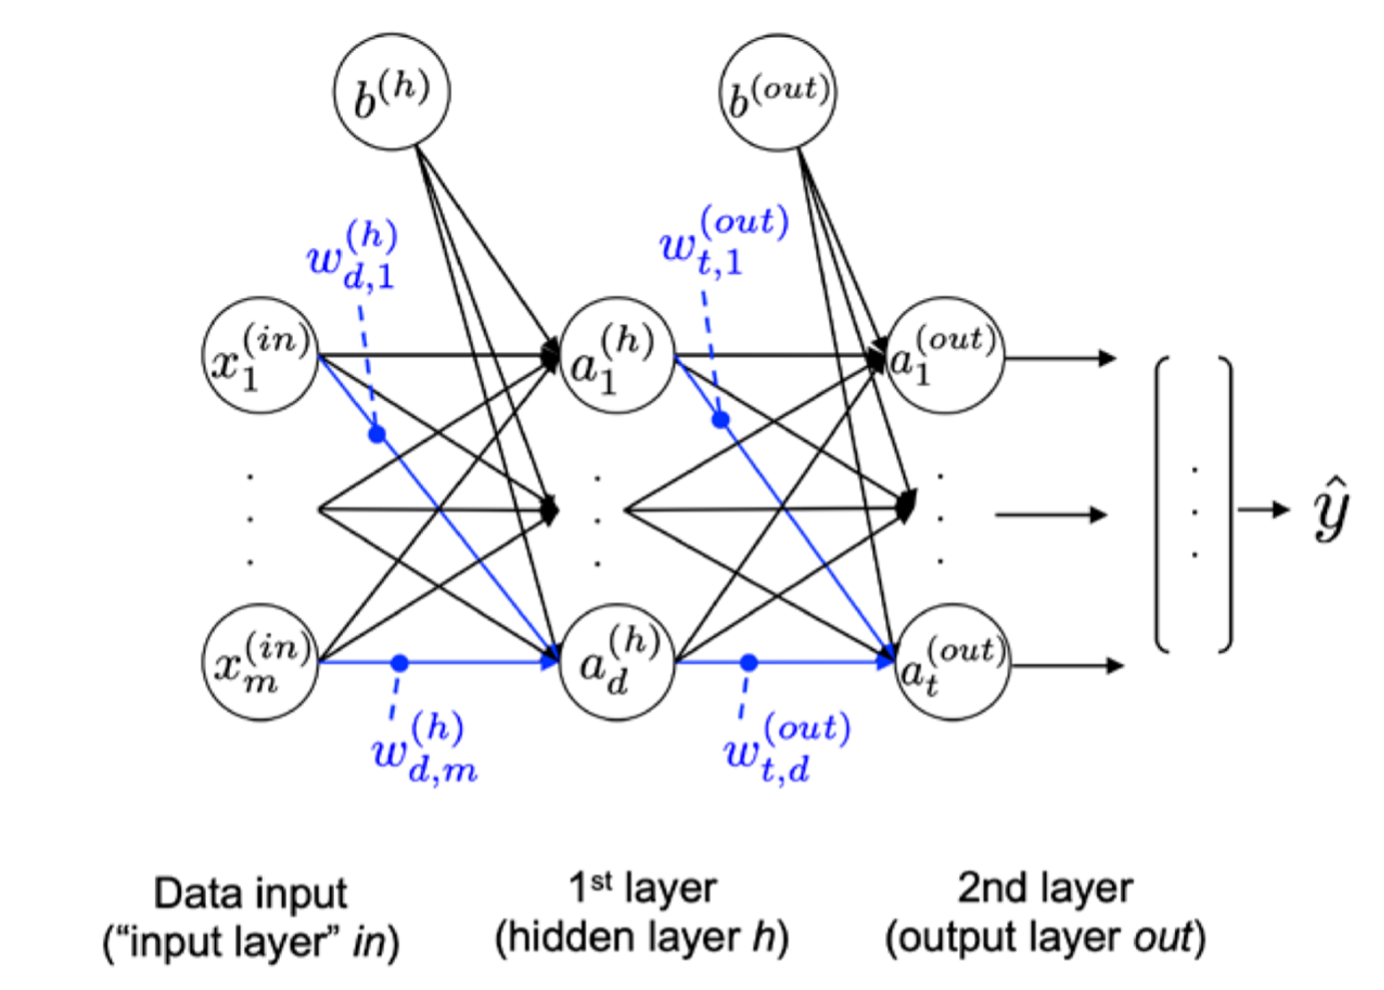
\includegraphics[width=0.8\textwidth]{FFNN.png}
  \caption{Illustration of a Multilayer feedforward Neural Network \parencite{Raschka2017}}.
  \label{neural_network}
\end{figure}

The architecture consists of nodes, or neurons, organized into three main layers: (1) the input layer, which receives the data, (2) one or more hidden layers, where data transformation and computation occur, and (3) the output layer, which produces the results. Each neuron in a layer is connected to every neuron in the subsequent layer through parameters known as weights, with additional parameters called biases contributing to the neurons' output. 

The first step in an MLP is to initialize the weights and biases, typically setting them to small random values. This randomness is important to break symmetry and ensure the model learns effectively. There are various strategies like \textit{Xavier} \parencite{glorot2010} or \textit{He} initialization \parencite{He_2015}, depending on the linearity or nonlinearity of the activation function, that can improve accuracy and training time.

The next step is forward propagation, which involves passing the input data through the network from the input layer, through the hidden layers, to the output layer. At each layer, the input is transformed by a weighted sum followed by an \textit{activation function}. This process results in the network's prediction based on the current state of its weights. Activation functions introduce nonlinearities into the model, enabling it to learn complex patterns. Commonly used activation functions include:

\begin{itemize}
  \item \textbf{ReLU}: $\sigma\left(z\right)=\max{\left(0,\ z\right)}$
  \item \textbf{GELU}: $\sigma\left(z\right)=\ z\ \ast\ P\left(Z\ \le\ z\right)=\ z\ \phi\ \left(z\right)=\ z\ \ast\ \frac{1}{2}\ \left[1\ +\ erf\left(\frac{x}{\sqrt2}\right)\right]
  if\ Z\ \sim N(0,\ 1)$
\end{itemize}

where $z$ is the net input from the network. Gaussian Error Linear Units (GELU) introduced by \cite{Hendrycks2016}, is presently the most common due to its performance. However, \cite{Raschka2017} highlights that the choice of activation function depends on whether it is a classification or a regression problem, network architecture, training speed and network performance.

After forward propagation, the network's performance is evaluated using a loss function (sometimes referred to as cost function or objective function). The choice of the loss function is an important hyperparameter of a neural network, where some, such as \cite{drager2022evaluating}, argue it is the most important. Some commonly used loss functions for regression problems include \textit{Mean Squared Error} and \textit{Mean Absolute Error}: 

\begin{itemize}
  \item \textbf{Mean Squared Error (MSE)}: $MSE=\frac{1}{n}\sum_{i\ =\ 1}^{n}\left(y^{\left(i\right)}\ -\ {\hat{y}}^{\left(i\right)}\right)^2$
  \item \textbf{Mean Absolute Error (MAE)}: $MAE=\frac{1}{n}\sum_{i\ =\ 1}^{n}\left|y^{\left(i\right)}\ -\ {\hat{y}}^{\left(i\right)}\right|$
\end{itemize}

Each loss function has its own pros and cons, including sensitivity to outliers, challenges in convergence, and more. For instance, the MAE is more resistant to outliers than the MSE because it calculates the average of absolute differences between predicted and actual values. This avoids the exaggerated impact that squaring the errors in MSE has on large deviations. Additionally, it is desirable for a loss function to be differentiable, as gradient descent relies on this property to update weights and biases effectively during backpropagation, steering the model toward minimizing the loss.

Backpropagation is the process of calculating the gradient of the loss function with respect to each weight and bias in the network. This is done by applying the chain rule of calculus and propagating the error backwards through the network. If we modify the MSE slightly with a normalization factor for convenience, as shown by \cite{Raschka2017}, the loss function for a simple classification problem can be defined as: 

\begin{equation}
  L\left(\textbf{w},\ b\right)=\ \frac{1}{2n}\sum_{i\ =\ 1}^{n}\left(y^{\left(i\right)}\ -\ \sigma\left(z^{\left(i\right)}\right)\right)^2
  \label{simplifiedloss}
\end{equation}

where $\textbf{w}$ is the weight vector, $b$ is the bias term, $y^{\left(i\right)}$ is the actual class and $\sigma\left(z^{\left(i\right)}\right)$ is the activation function applied to the net input. The net input has the following definition:

\begin{equation}
  z^{(i)}\ =\ \textbf{w}^\textbf{T}x^{(\textbf{i})}\ +\ \textbf{b}\ =\ \sum_{\textbf{i}=\textbf{1}}^{\textbf{m}}{\textbf{w}_\textbf{j}\ \ast\ \textbf{x}_\textbf{j}^{(\textbf{i})}+\textbf{b}}
\end{equation}

where $x^{(\textbf{i})}$ is the feature vector of the \textit{i}-th sample and $m$ is the total number of features. This can then be used to compute the partial derivative of this loss function with respect to each weight $w_j$ in the weight vector and bias:

\begin{equation}
  \frac{\partial L}{\partial w_j}\ =\ -\frac{1}{n}\sum_{i=1}^{n}\left(y^{\left(i\right)}\ -\ \sigma\left(z^{\left(i\right)}\right)\right)\sigma'\left(z^{\left(i\right)}\right)x_j^{\left(i\right)}
\end{equation}

\begin{equation}
  \frac{\partial L}{\partial b}\ =\ -\frac{1}{n}\sum_{i=1}^{n}\left(y^{\left(i\right)}\ -\ \sigma\left(z^{\left(i\right)}\right)\right)\sigma'\left(z^{\left(i\right)}\right)
\end{equation}

Here, $\sigma'\left(z^{\left(i\right)}\right)$ is the partial derivative of the activation function. The process repeats numerous times to train the network and minimize the errors. It works as the derivative tells what direction the function is growing, and we take a step in the opposite direction, where the learning rate and the slope of the gradient determine the size. Thus, the updating of the weight and bias terms are defined as:

\begin{equation}
  \triangle w_j = -\eta\frac{\partial L}{\partial w_j}
\end{equation}

\begin{equation}
  \triangle b = -\eta\frac{\partial L}{\partial b}
\end{equation}


where $\eta$ is the learning rate. There are also more optimized gradient descent methods, such as mini-batch and stochastic gradient descent, designed to speed up the process. Furthermore, several issues should be considered when using gradient descent, such as the learning rate $\eta$. If too small, the optimization can get “stuck” in local minima; if too large, it can overshoot the global minima. Stochastic gradient descent is often used in practice due to its performance and computational desirability.

Adam optimisation has emerged as particularly popular among the various optimization techniques that build upon traditional gradient descent. Adam optimization, introduced by \cite{Kingma2014AdamAM}, is a technique for gradient descent optimization that has gained popularity in deep learning due to its computational efficiency, low memory requirements, and minimal manual tuning. It does so by combining two previous ideas, Momentum and RMSprop. Momentum accelerates gradient descent by considering previous gradients to smooth the update. At the same time, RMSprop modifies the learning rate for each parameter by dividing it by an exponentially decaying average of squared gradients. Adam also incorporates a decaying learning rate mechanism, gradually reducing the learning rate as training progresses. These features make Adam particularly effective for training deep neural networks.

\subsubsection{Recurrent Neural Networks}

Feed-forward neural networks excel at mapping one-to-one relationships between inputs and outputs. However, they struggle with sequential data, where the output depends on a sequence of previous elements. \textit{Recurrent Neural Networks} (RNN) possess an internal memory state, enabling them to retain information from previous inputs. This design allows them to process sequences, making them suitable for tasks such as language translation and time series forecasting. In this context, we will concentrate on what is known as the $Vanilla$ $RNN$, which was once commonly employed for language-related tasks.

At the heart of RNNs is the internal memory state at each time step. \cite{Staudemeyer2019} explains that this mechanism is made possible with hidden layers with a self-looping workflow, meaning the hidden layers can remember previous inputs and use these to make predictions. Predictions are made with the current input, the learned weights and biases, and the stored memory of the hidden layers.

% \begin{figure}[htbp]
%   \centering
%   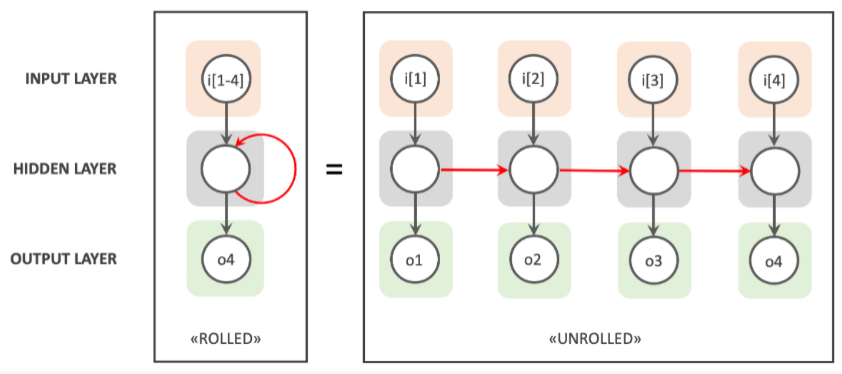
\includegraphics[width=0.8\textwidth]{RNN.png}
%   \caption{Illustration of a RNN \parencite{bouvet}}.
%   \label{rnn}
% \end{figure}

\cite{Staudemeyer2019} underline that RNNs need different training than normal feedforward networks, where the most common method is backpropagation through time (BPTT). \cite{werbos1990backpropagation} introduced BPTT, however, mainly within the task of pattern recognition and other methods than neural networks. \cite{Raschka2017} describe BPTT as distinct from standard backpropagation because it feeds the output from one time step back into the network, allowing errors to be recalculated and temporal dependencies to be accounted for. It can do so by computing the gradients for each step while considering the weights of the loss at each step. Using the simplified definition above for the loss function (\ref{simplifiedloss}) with time indices, the loss function is:

\begin{equation}
  L\left(\textbf{w},\ b\right)=\ \frac{1}{2n}\sum_{i\ =\ 1}^{n}\sum_{t=1}^{T}\left(y_t^{\left(i\right)}\ -\ \sigma\left(z_t^{\left(i\right)}\right)\right)^2
  \label{simplifiedlosstime}
\end{equation}

Where $y_t^{\left(i\right)}$ is the actual output at time $t$ and  $\sigma\left(z_t^{\left(i\right)}\right)$ is the predicted at time $t$. As it must consider output from previous layers as well, the gradient will be defined as:

\begin{equation}
  \frac{\partial L^{\left(t\right)}}{\partial\textbf{w}_{hh}}\ =\ \sum_{k\ =\ 1}^{t}\left(\frac{\partial L^{\left(t\right)}}{\partial\textbf{o}^{\left(t\right)}}\ast\frac{\partial\textbf{o}^{\left(t\right)}}{\partial h^{\left(t\right)}}\ast\frac{\partial h^{\left(t\right)}}{\partial h^{\left(k\right)}}\ast\ \frac{\partial h^{\left(k\right)}}{\partial\textbf{w}_{hh}}\right)
  \label{rnngradient}
\end{equation}

$L^{\left(t\right)}$ represents the loss at time $t$, $\textbf{o}^{\left(t\right)}$ is the output of the network at time $t$ and $h^{\left(t\right)}$ is hidden state of the network at time $t$. $\textbf{w}_{hh}$ is a matrix that connects the hidden states with the hidden layers at the next time step, sharing the weights across the network, thereby making it recurrent. This process fine-tunes the model's ability to learn from the sequence's context, ultimately improving its prediction accuracy.

However, due to multiplicative effects, RNNs face challenges with exploding/vanishing gradients. \cite{Gers2000} report RNNs are generally limited to looking back in time for approximately 5-10 timesteps. Because of this limitation, traditional $Vanilla$ $RNNs$ are rarely used. Nevertheless, more sophisticated architectures derived from RNNs, like Long Short-Term Memory networks, effectively address these challenges and remain relevant.

\subsubsection{Long Short-Term Memory Networks}
Long Short-Term Memory networks (LSTMs), introduced by \cite{Hochreiter1997}, are an advanced type of RNNs designed to address the challenges of exploding and vanishing gradients in standard RNNs. Unlike traditional RNNs, which struggle with learning long-term dependencies due to gradient issues, LSTMs are adept at retaining information over longer sequences. \cite{Staudemeyer2019} reports up to 1,000 steps, making them suitable for complex tasks such as time series forecasting.

The constant error carousel is a fundamental concept in LSTM networks, addressing the vanishing gradient problem. The constant error carousel is achieved through its unique cell state structure. The cell state in an LSTM is a longitudinal component that carries relevant information throughout the sequence of the network, enabling the retention and selective modification of information over long periods. It carries the network's memory, allowing information to be passed along unchanged if necessary \parencite{Staudemeyer2019}. This is done by the LSTM's gated structure, which regulates the information added to or removed from the cell state.

\begin{figure}[htbp]
  \centering
  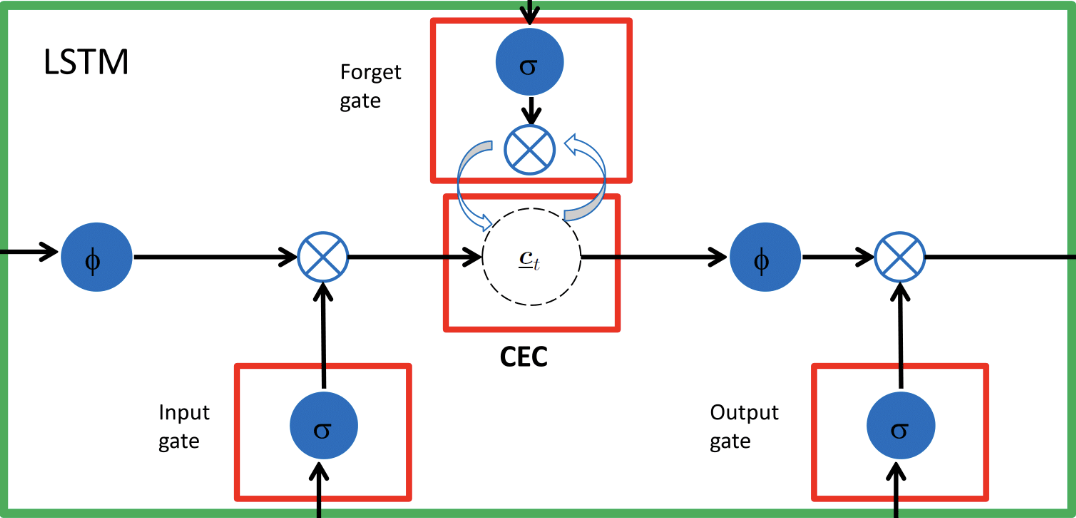
\includegraphics[width=0.8\textwidth]{lstm_illu.png}
  \caption{Illustration LSTM Memory Block \parencite{lstmsu2018}}.
  \label{lstmmemoryblock}
\end{figure}

At the core of LSTM's architecture are memory blocks, depicted in Figure \ref{lstmmemoryblock}, which replace the standard neurons found in RNNs. These memory blocks are equipped with the following arrangement of gates: (1) the forget gate, (2) the input gate, and (3) the output gate. The forget gate is responsible for deciding which information to discard from the block's memory, effectively "forgetting" irrelevant data. The input gate controls the addition of new information to the memory, updating the cell state with inputs. The output gate then determines the next hidden state, considering the current input and the block's memory \parencite{Staudemeyer2019}.

LSTMs use a mixed learning method that combines different training approaches for better results. Importantly, forget gates decide what information to keep or remove, focusing on relevant data. In the backward step, the network uses BPTT to adjust weights based on learning from errors \parencite{Staudemeyer2019}. Although LSTMs are good at learning from long data sequences and avoid issues with vanishing and exploding gradients, they require a lot of computing power and can be complex to fine-tune.

\subsubsection{Convolutional Neural Networks}
AlexNet by \cite{Krizhevsky2012} marked a breakthrough in computer vision. This neural network was made possible with convolutions. The origins of \textit{Convolutional Neural Networks} (CNN) go back to 1989 when it was first introduced by Yann LeCun and his colleagues in \textit{Handwritten Digit Recognition with a Back-Propagation Network}. Despite the innovation of the transformer, which now can outperform CNNs in computer vision tasks, CNNs remain one of the most influential predecessors. They are still used in various applications beyond computer vision \parencite{deininger2022comparative}.

At the heart of CNNs are convolutional layers. A \textit{convolution} is an operation used to combine an input with a filter, also known as a \textit{kernel}, to produce a feature map. This operation highlights patterns or features in the input data. In a discrete convolution, the kernel slides over the input data, performing element-wise multiplications with the covered part of the input at each position. The results of these multiplications are summed to produce a single output value, forming the output feature map \parencite{Raschka2017}.

For example, consider a two-dimensional input matrix $X$, representing time series data, and a kernel matrix $W$. The convolution operation can be expressed as:

\begin{equation}
  Y\ =\ X\ \ast\ W\ \rightarrow\ Y_{i,\ j}\ =\ \sum_{k1\ =\ -\infty}^{+\infty}\sum_{k2\ =\ -\infty}^{+\infty}{X_{i\ -\ k1,\ j\ -\ k2}W_{k1,\ k2}}
\end{equation}

Here, $X$ is the input matrix, and $W$ is the kernel matrix. Infinite bounds are not used in practical applications; padding is applied. Padding involves adding a finite number of zeros around the input matrix, ensuring that the indices remain within a valid range \parencite{Raschka2017}. This allows the convolution to handle edge values appropriately and maintain the spatial dimensions of the input data.

In addition to convolutional layers, CNNs often incorporate pooling layers, which help to reduce the dimensionality of the feature maps. Pooling layers perform a down-sampling operation along the spatial dimensions of the input, which simplifies the information and reduces the computational load for subsequent layers \parencite{Raschka2017}. This operation helps detect certain features invariant to scale as it introduces local invariance and increases robustness to noise \parencite{Raschka2017}.

This operation can be particularly useful for time series data. By applying a convolution across a time series, the model can detect patterns or features, like trends or seasonal effects, over sliding windows of the series, making it valuable for forecasting tasks.

\subsection{Transformer-Based Models}
In deep learning, CNNs and LSTMs have historically dominated the scene, particularly for processing sequence data. However, a shift occurred when \cite{Vaswani2017} from Google Brain and Google Research released \textit{Attention Is All You Need}, which introduced the \textit{transformer model}. The model has become a cornerstone in deep learning, particularly in NLP, gaining widespread adoption among tech giants such as Google, OpenAI, Microsoft, and Nvidia. Transformer-based models encompass a wide range of architecture that utilize the transformer mechanism for processing data. One notable subset of these models is OpenAI's \textit{Generative Pre-trained Transformers} (GPTs). 

Before transformers, RNNs, including LSTM units and Gated Recurrent Units (GRUs), were the preferred solutions for sequential data. These models, however, faced limitations in their ability to process information from a long series of data due to their fixed reference window, which restricted how far back they could look to make predictions. While LSTMs mitigated some of these challenges, they did not completely overcome them. Additionally, the computational demands for RNN-based models scaled exponentially with task complexity, posing practical limitations for their application in real-world scenarios.

Transformers introduced a revolutionary approach with their theoretically infinite reference window, allowing them to consider all available data points when making predictions. This capability marked significant progress in NLP and showed promise for application in time series forecasting despite the differences between these fields. Moreover, the transformer architecture facilitated parallel processing during training, drastically reducing the computational resources required. This innovation addressed the scalability issues previous neural network models faced and opened new gateways for research and application in various domains beyond NLP. 

\subsubsection{Architecture}
The Transformer model’s architecture comprises an \textit{encoder} and a \textit{decoder}. Typically, the input of a neural network is called a \textit{token}. While practitioners and scholars seem to lack agreement on this for time series, we will use this term. The encoder processes the input token, encoding it into a high-dimensional space where relationships are captured through layers of self-attention and feed-forward networks. The decoder then uses this encoded information to generate future values in the series, leveraging its self-attention layers to maintain internal coherence and encoder-decoder attention layers to focus on relevant input parts. The training of a transformer model is much the same as that of other neural networks, where gradient descent plays a vital role. 

\begin{figure}[htbp]
  \centering
  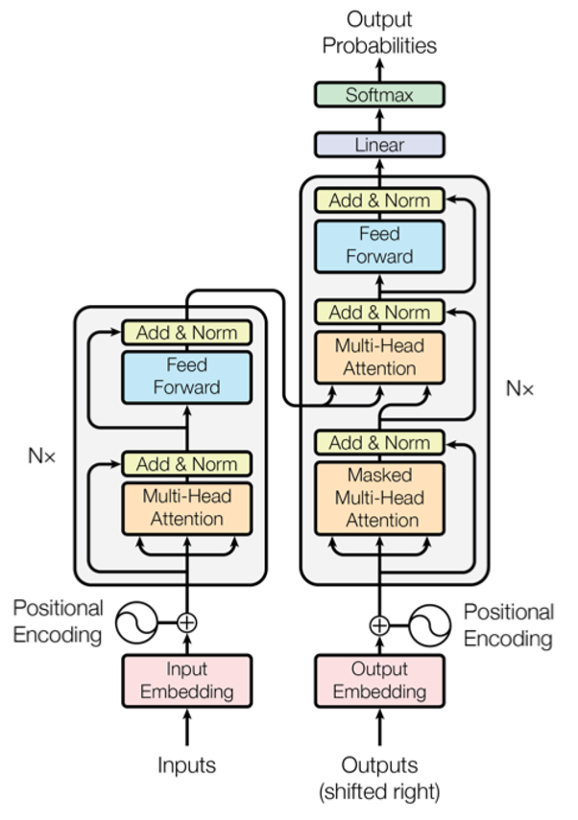
\includegraphics[width=0.6\textwidth]{transformer.png}
  \caption{Illustration of the original Transformer model from \cite{Vaswani2017}.}
  \label{transformer}
\end{figure}

\paragraph{Positional Encoding and Embedding}
Because transformers do not process tokens sequentially, such as an RNN or CNN, the model needs to understand the order in a different manner. To solve this, \cite{Vaswani2017} uses \textit{embedding} and \textit{positional encoding}.

Embedding is a pre-processing step that translates raw data into a numerical representation suitable for neural network models. In NLP, embedding converts textual elements, such as words or phrases, into vector representations. Techniques like Word2Vec are widely employed to achieve this transformation. These vectors capture the semantic relationships between words, allowing the model to determine the meaning of a word based on its context. For time series data, this would extend to time series attributes such as seasonality, cycles, and stationarity.

Positional encoding supplements the embedding vectors with additional information that captures the relative position of each element within the sequence. This additional information allows the model to retain the sequential information and understand how the elements relate. In \cite{Vaswani2017}, they use sine and cosine functions for positional encoding:

\begin{equation}
  PE_{(pos,2i)}\ =\ \sin\left(\frac{pos}{10000^{2i/d_{model}}}\right)
\end{equation}

\begin{equation}
  PE_{(pos,2i+1)}\ =\ \cos\left(\frac{pos}{10000^{2i/d_{model}}}\right)
\end{equation}

Where $pos$ is the position, $i$ is the dimension, and $d_{model}$ represents a dimension of the models’ embeddings, meaning that if a token is represented by a 512-dimensional vector, $d_{model}$ would equal 512. Note the difference in the subscript as the $sine$ function is applied to those at even positions, and $cosine$ is applied to those at odd positions. 

\paragraph{Encoder and Decoder}
The encoder is the first component of a transformer model and is responsible for processing and understanding the input sequence. It consists of multiple encoding layers containing a \textit{self-attention mechanism} (discussed in detail below) and a feed-forward network. The feed-forward network is a simple neural network that is used to refine the representation of the input token further, enabling the model to capture non-linear relationships and transformations in the token. 

In the transformer architecture, depicted in Figure \ref{transformer}, each of the sub-layers within a transformer block, which includes the multi-head attention layer and the position-wise feed-forward network, is followed by \textit{layer normalization}, a technique introduced by \cite{ba2016layer}. Specifically, the output of each sub-layer passes through a residual connection that adds the sub-layer input to its output, and the layer normalization then normalizes this combined output. The layer normalization ensures that each component output is standardized before passing to the next layer or sub-layer, contributing to the model's effectiveness and stability. \cite{Vaswani2017} highlights that normalization helps stabilize the learning process by ensuring consistent scale and mean of activations across the network's depth. 

\paragraph{Attention in Transformers}
Central to transformer models is the mechanism of attention. \cite{bahdanau2016neural} first introduced in their work to improve the performance of machine translation. The mechanism involves computing alignment scores between different points in the data. These scores indicate the relevance or importance of each data point when predicting a future value. The model then creates a context vector for each predicted point, a weighted sum of the data, with weights derived from the alignment scores. The alignment scores are typically calculated using the hidden states from a recurrent neural network or another model framework, reflecting the relationship between each point.

Contrastive to models such as RNN, which relies on sequential processing, \cite{Vaswani2017} reports transformers can focus on different parts of the input sequence in parallel, irrespective of their position, using self-attention. When applied to time series, it enables each point in the series to attend to all other points, in contrast to traditional time series models that often rely on a fixed window of recent data. Processing all points in a time series in parallel offers a significant efficiency advantage.

The model generates three vectors for each point: a $query$ vector, a $key$ vector, and a $value$ vector. These are produced from the same data point but are transformed differently. One can consider these in the following way: $queries$ is an inquiry to find some specified information stored in $keys$, and when matched, they return a $value$. While this is highly simplified, it encapsulates the logic of the attention mechanism, which for time series is finding points relevant to the value at hand. To do this, \cite{Vaswani2017}, uses \textit{Scaled Dot-Product} (multiplicative) \textit{Attention}. This is computed using the following formula:

\begin{equation}
  Attention(Q,\ K,\ V)\ =\ \text{SoftMax}\left(\frac{QK^T}{\sqrt{d_k}}\right)V
  \label{attention}
\end{equation}

In practice, the $queries$, $keys$, and $values$ are matrices. $QK^T$ represents the matrix product of the $query$ matrix and the transpose of the $key$ matrix. The scaling, dividing by $\sqrt{d_k}$ (the square root of the vector length), is applied to avoid issues with unsuitably small gradients from the SoftMax. An optional feature of the attention mechanism is \textit{masking}. \cite{Vaswani2017} uses masking in this context to prevent the model from accessing future values of the input sequence when computing the attention score for $i$, ensuring the prediction only has “known” values. This step is done before the SoftMax function is applied. The output is a sum weighted by the $value$ matrix, describing the relationship and dependency of the order, reflecting how the different points pay “attention” to each other. In practice, \textit{Multi-Head Attention} is used, where this process is done multiple times in parallel to capture information from different positions. This translates to:

\begin{equation}
  \text{MultiHead}(Q,\ K,\ V)\ =\ \text{Concat}\left(\text{head}_1,\ \ldots,\ \text{head}_h\right)W^O
  \label{multihead}
\end{equation}


Where ${head}_i\ =\ Attention\left(QW_i^Q,\ KW_i^K,\ VW_i^V\right)$ and $W_i^Q$, $W_i^K$, and $W_i^V$ are weight matrices and $W^o$ is the weights of the output. The number of heads, or attention layers, is a specified parameter. Because the outputs of all attention heads are concatenated and then multiplied with the output weights, the model can draw insights from all heads. 

\begin{figure}[htbp]
  \centering
  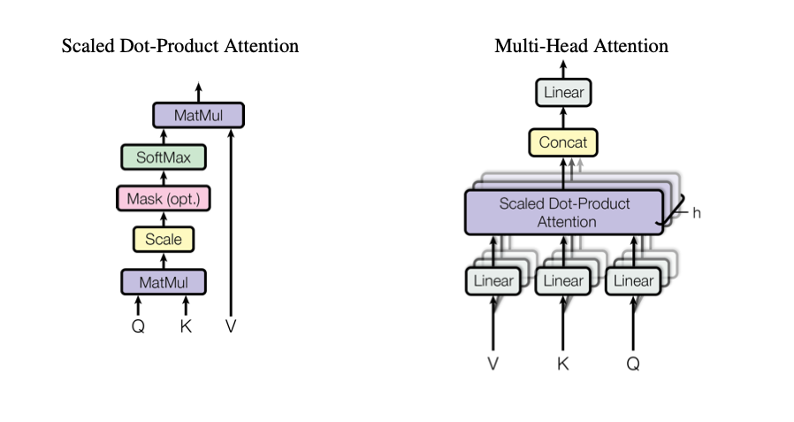
\includegraphics[width=0.8\textwidth]{attention.png}
  \caption{Illustration of Multi-Head Attention \parencite{Vaswani2017}}.
  \label{multiheadattention}
\end{figure}

\subsubsection{Inference}
After the transformer is trained, it is ready for inference. The entire input sequence is provided to the encoder, which processes it all simultaneously and generates a series of encoder outputs. These outputs capture the contextual relationships within the input sequence. \cite{youtube} explains that the inference process begins in the decoder with an initial start-of-sequence (SOS) token. This token and the encoder outputs are fed into the decoder. The decoder then generates the first output token by processing the combination of the SOS token and the encoder outputs through its layers.

This output from the decoder is transformed by a linear layer followed by a SoftMax function, which translates it into a probability distribution over the possible following tokens. The token with the highest probability is selected as the output. The decoder takes the previously generated tokens, and the encoder outputs them as input for each subsequent token. This process is repeated, with the decoder generating one token at a time until it produces an end-of-sequence (EOS) token or completes the sequence. Each decoder output is subject to the same linear and SoftMax transformation to determine the next token in the sequence. This sequential generation continues until the entire output sequence is produced.

\subsubsection{Transfer Learning}
In traditional machine learning, the training and test data are expected to be very similar, with the same input feature space and data distribution. However, a limited supply of training data can occur due to the data being limited, rare or expensive to collect and label. According to \cite[1--2]{Weiss2016}, this introduced the need for \textit{transfer learning} as a capacity to apply knowledge from a related source domain to the target domain. This is particularly important for foundation models, like our transformer-based models, as they rely on generalizing across domains, even on new datasets on which they have not been trained. As illustrated in Figure \ref{transferlearning}, traditional machine learning has a one-to-one relationship between each task and learning system, while transfer learning aims to utilize knowledge from multiple source tasks in a learning system on a new target task.

\begin{figure}[htbp]
  \centering
  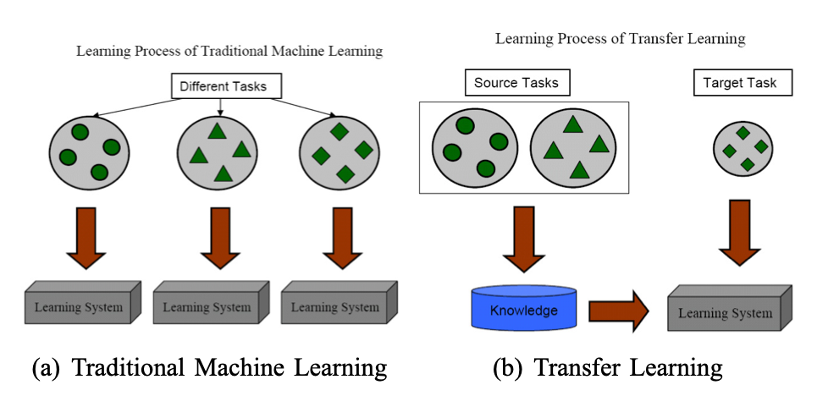
\includegraphics[width=0.8\textwidth]{transferlearning.png}
  \caption{Illustration of Transfer Learning \parencite{Pan2010}}.
  \label{transferlearning}
\end{figure}

Foundation models aim to use knowledge from pre-trained data to handle various tasks. By training on a vast amount of diverse data, these models learn patterns and relationships that can be applied to different areas. This is helpful when labeled data is hard to get or expensive because it allows the models to work well on new tasks with minimal extra training. Transformers can be trained with supervised and unsupervised learning. In supervised learning, the model is trained on labeled data, while in unsupervised learning, the model is trained on unlabeled data.

However, a limitation of foundation models is the training. Foundation models require extensive pre-training datasets and are computationally intensive, which can make training time-consuming, often requiring days or weeks, despite efforts to optimize the training process \parencite{Ivanov2020,Yang2022}.

\subsubsection{Transformers for Time Series Forecasting}

Recent research in the field of transformer models for time series forecasting highlights efforts to modify the architecture to suit this task better. This research has led to several suggested architectures. Consider how a transformer model processes text to motivate these changes in the architecture. In textual data, the model needs to grasp the relationships between words to understand longer contexts, and it achieves this through the attention mechanism. For example, consider the sentence: "\textit{I wish your help in the project I am working on}". It still conveys the same meaning if we rephrase it to: "\textit{I am working on a project, and I need your help}". Ideally, a transformer model should understand both sentences equally well despite the different word order. However, with time series data, the order of the data points is crucial. Imagine a fictitious series representing daily temperatures over a week: \textit{[21, 23, 20, 22, 24, 25, 21]}. Reordering this to \textit{[25, 21, 23, 20, 24, 22, 21]} would distort the entire trend and lead to incorrect insights.

In other words, while transformers can handle word reordering in text data, reordering can destroy meaning in time series data. Adapting the transformer architecture aims to capture temporal dependencies more precisely. This objective has led to innovative approaches within the transformer framework, such as the Autoformer by \cite{wu2021autoformer}.

Autoformer advances the architecture by incorporating an automatic decomposition mechanism that separates the series into trend and seasonal components before processing. \cite{wu2021autoformer} report that this decomposition allows the model to focus on the underlying trend by applying a series-wise auto-correlation window, improving the forecasting accuracy for time series with strong seasonal patterns. Additionally, Autoformer redesigns the self-attention framework to integrate a frequency-enhanced attention mechanism that aids in distinguishing between different frequencies of time series data, thereby enhancing the capture of temporal dependencies.

Another proposed architecture to better suit time series forecasting is the Informer model by \cite{Zhou2020}. This model addresses the inefficiencies in standard self-attention mechanisms, which scale poorly with longer time sequences due to quadratic computational complexity. \cite{Zhou2020} introduces a sparsity mechanism in the attention module, termed "ProbSparse Self-Attention". This attention mechanism selectively activates the most informative parts of the data, reportedly reducing the computational load without sacrificing performance. This makes it suitable for processing very long time series efficiently. Furthermore, the Informer employs a distilling operation that further compresses the sequence length during the attention process, enhancing its ability to capture temporal dependencies.

These adaptations aim to address the main limitation of the original transformer design: its inability to maintain order in the data, which is crucial for accurate time series forecasting. Refining and adjusting the architecture makes the transformer model aims to make it more adept at time series forecasting. 

On the other hand, \cite{zeng2022transformers} critically examines the applicability of transformers to time series forecasting. While natural language tasks rely on the sequential order of words, time series forecasting demands precise handling of time series—a challenge for transformers due to their self-attention mechanism, which is relatively insensitive to the order of inputs, potentially leading to the loss of time series attributes. \cite{zeng2022transformers} demonstrate that despite their sophisticated architecture, transformers can underperform compared to simpler models, such as a basic one-layer linear model, particularly in long-term time series forecasting scenarios. This juxtaposition raises questions about the practical effectiveness of transformers in time series contexts, calling for further adaptation in the field.

Moreover, \cite{zeng2022transformers} explore various aspects of transformer design that impact their ability to extract temporal dependencies. Their studies show that modifications to the self-attention mechanism intended to capture time series attributes better do not necessarily overcome its fundamental limitations. They conclude that the effectiveness of transformers for long-term time series forecasting is overstated and recommend reassessing their use in time series analysis, especially in cases where accurate modeling and understanding of time-related patterns are crucial.

These findings underscore the need for continued development and evaluation of time series forecasting models. They question the reliance on complex architectures like transformers when simpler, more interpretable models may be sufficient.

\subsection{TimeGPT}

TimeGPT is a foundation model for time series data developed by the company Nixtla and was introduced by \cite{garza2023timegpt1}. Unlike open-source projects, TimeGPT is commercially driven, which results in limited technical documentation. Nevertheless, this section aims to provide an overview of the model's architecture, training, how it creates forecasts and other capabilities. The version of TimeGPT relevant to this thesis is TimeGPT-1.

\subsubsection{Model Architecture}

TimeGPT’s architecture, depicted in Figure \ref{timegpt}, is similar to that of \cite{Vaswani2017}. However, some key elements differ. Naturally, it does not output probabilities from a SoftMax function; instead, the last layer is linear to output predicted continuous values. Furthermore, where the original transformer uses feed-forward networks, TimeGPT has replaced this with convolutional neural networks. However, it is not specified in any way how this is used or why. \cite{garza2023timegpt1} also underlines that it is not based on any existing LLM and that it is specialized to handle time series data with the goal of minimizing forecasting error. Apart from this, \cite{garza2023timegpt1} does not reveal any other significant differences in the model architecture.

\begin{figure}[htbp]
  \centering
  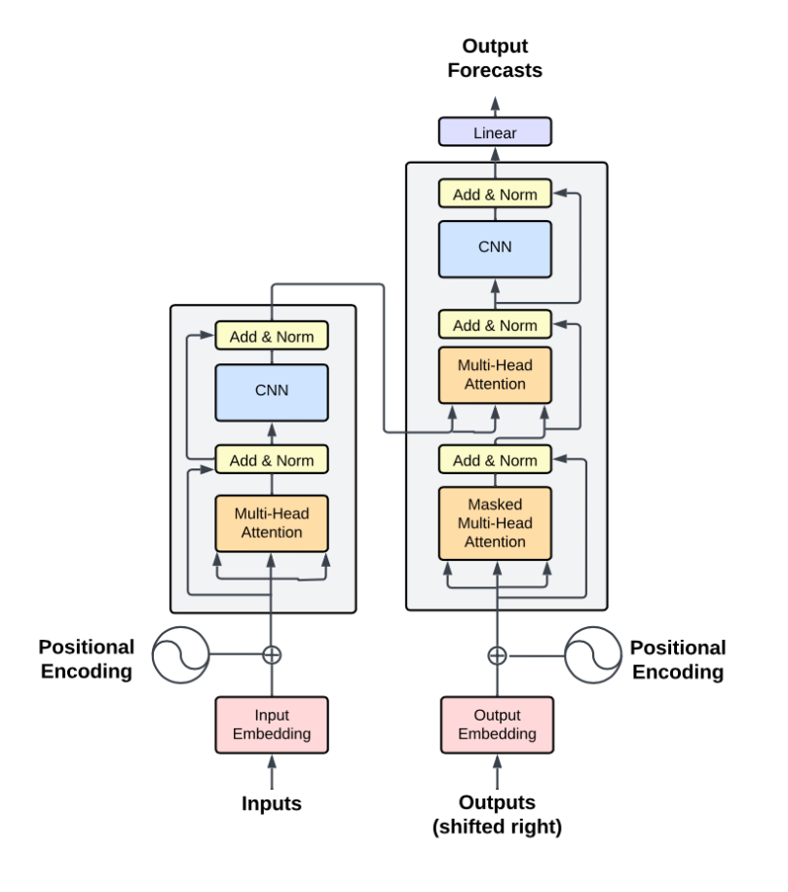
\includegraphics[width=0.8\textwidth]{timegpt_fig.png}
  \caption{Model architecture of TimeGPT \parencite{garza2023timegpt1}}.
  \label{timegpt}
\end{figure}

\subsubsection{Training}

\cite{garza2023timegpt1} claims that TimeGPT was trained on the largest publicly available time series dataset as of 5. November 2023 with more than 100 billion observations. The data is reportedly from various domains such as finance, health, industry, sales, IoT sensors, energy, transport, weather, etc. It is mentioned that the data contains several different forms of seasonality and cycles, representing non-stationary real-world data. Regarding preprocessing, it is only noted that it was formatted to a standard and that missing values were filled in. It is unclear how this was done, whether by imputing the mean, median, or another method. In addition, no statistics such as time frequency about the data is reported. 

In the training of the model, they mention that hyperparameters such as the learning rate and batch sizes were explored and tampered with extensively. In addition, they do mention that it was trained using the Adam optimizer with a decaying learning rate (described in \ref{neuralnetworks}). 

\subsubsection{Approach to Time Series Forecasting}

TimeGPT's approach to forecasting involves reading time series data as a sequence of tokens. With a target variable and the possibility of including events and additional variables, TimeGPT can process input data to create forecasts \parencite{Nixtla}.

\begin{figure}[htbp]
  \centering
  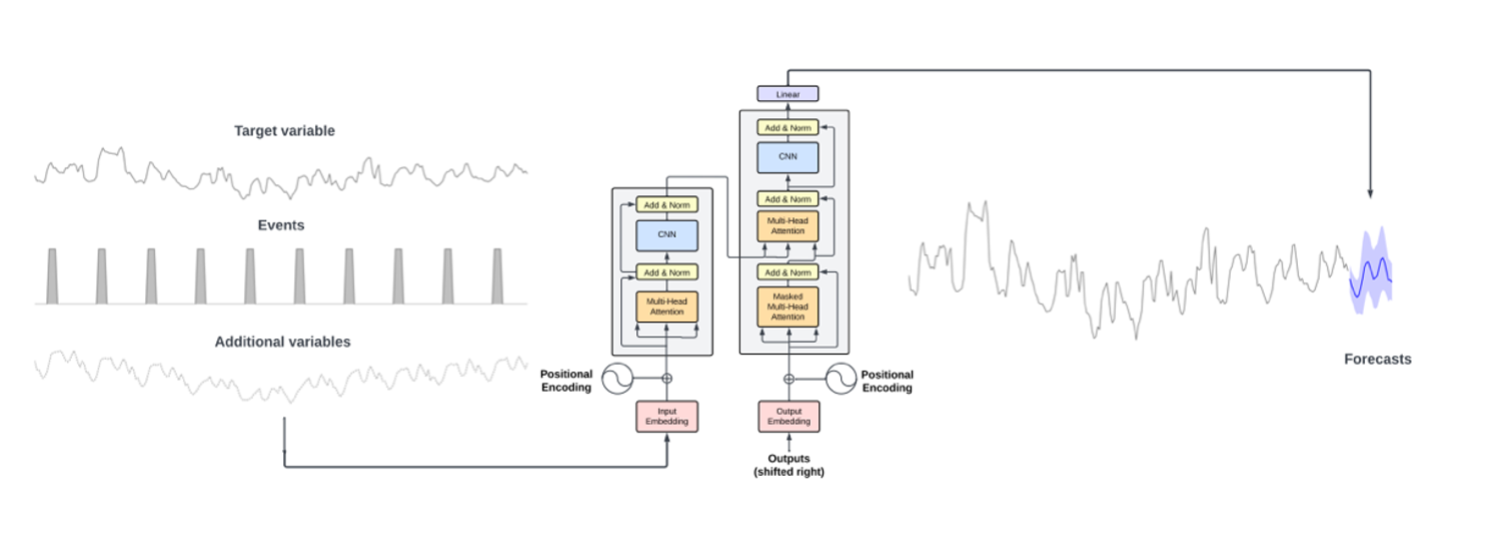
\includegraphics[width=0.8\textwidth]{timegpt_forecast.png}
  \caption{The Forecasting Pipeline of TimeGPT \parencite{garza2023timegpt1}}.
  \label{timegptforecast}
\end{figure}

As the model ingests time series data, it processes the information in chunks, transforming raw numerical inputs into discrete tokens that serve as input. As mentioned earlier, TimeGPT utilizes a structure of CNNs and multi-head attention mechanisms, supposedly allowing it to focus on different parts of the time series and appropriately weigh their significance when making predictions.

The model utilizes transfer learning with its pre-trained foundation. As explained earlier, the model is exposed to diverse time series datasets across various domains. This exposure enables the model to transfer the knowledge acquired during training to create forecasts for new, unseen time series. The pre-trained foundation aims to equip TimeGPT with an understanding of time series behaviors to empower the model to adapt to new time series data quickly. \cite{garza2023timegpt1} claims it allows TimeGPT to generalize across different fields without extensive retraining or fine-tuning, although fine-tuning can enhance model performance.

\subsubsection{Available Methods and Capabilities}

TimeGPT offers several capabilities, such as anomaly detection and the inclusion of exogenous variables. In this thesis, we are primarily interested in its zero-shot forecasting ability. Additionally, we conducted a small experiment using fine-tuning. For the fine-tuning experiment, please see \hyperref[appendix_d]{Appendix D}.

\subsection{Chronos}

\cite{ansari2024chronos} introduced Chronos, a set of multiple pre-trained time series forecasting models. It is inspired by the success of large language models (LLMs) and uses existing transformer-based language model architecture for time series. Chronos is open source, as it is freely available and collaborative to the public. Amazon Web Services developed Chronos in collaboration with UC San Diego, the University of Freiburg, and Amazon Supply Chain Optimization Technologies. 

\subsubsection{Model Architecture}

Chronos follows a minimalistic approach, utilizing an existing model architecture, the Text-to-Text Transfer Transformer (T5) by \cite{Raffel2019}. The only difference between Chronos and the original T5 is the vocabulary size, which is the number of tokens a model recognizes and utilizes to process and generate, resulting in fewer parameters. T5 has no time-series-specific features or design. The authors behind Chronos questioned whether any design modifications were essential for effective forecasting. Thus, \cite{ansari2024chronos} developed Chronos using a language modeling framework with minimal adaptations for time series forecasting.

The architecture for T5 is close to that of \cite{Vaswani2017}. The main differences in architecture are that T5 apply a simplified layer normalization, placing this layer before the feed-forward and attention components and utilizing a simpler scheme for positional encoding. The impact of the modifications made from the original transformer architecture has not yet been fully explored. However, given that these changes were considered minor in the research conducted by \cite{Raffel2019}, it is reasonable to assume that they will also be insignificant for this thesis.

\subsubsection{Training}

The Chronos models are trained on the base of a large set of publicly available datasets spanning multiple domains. This totals 28 datasets consisting of 893,208 time series. There is also variety in the time intervals for the time series, ranging from five-minute intervals to monthly intervals. The authors used data augmentation techniques to artificially enhance the training data to create a more robust foundation for the model. For the Chronos models, data augmentation includes (1) Time Series Mixup and (2) Synthetic Data Generation. Time Series Mixup (TSMix) randomly samples time series from the training data and scales them before combining them into a new time series. This improves pattern diversity. However, as the authors do not deem it sufficient to create a generalist time series model, they further generate synthetic data using Gaussian processes with the method KernelSynth. This method uses the underlying structures of the training data to create new time series'. This resulted in the Chronos models being trained on 10M TSMix augmentations and 1M synthetic time series generated with KernelSynth. Both TSMix and KernelSynth are innovations introduced by \cite{ansari2024chronos}.

\begin{figure}[htbp]
  \centering
  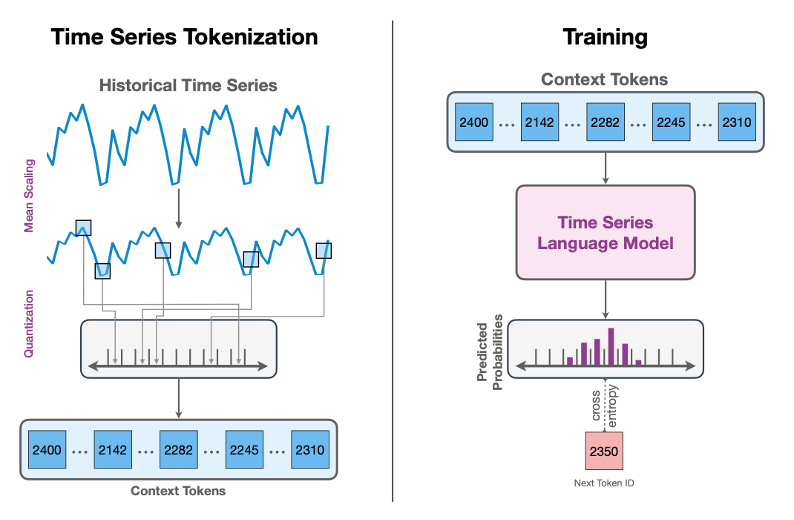
\includegraphics[width=0.8\textwidth]{chronos_training.png}
  \caption{High-level Depiction of the Training of Chronos \parencite{ansari2024chronos}}.
  \label{chronostraining}
\end{figure}

Data from the M4 Competition is used to pretrain the Chronos models and conduct an in-domain evaluation. However, data from the M3 Competition is only used for zero-shot evaluation by \cite{ansari2024chronos}, meaning that the model is not pre-trained on the data used in this thesis.

\subsubsection{Approach to Time Series Forecasting}

As previously mentioned, the T5 architecture was designed to handle text. It processes text by breaking it down into tokens and generating responses with tokens that are contextually relevant to the input. Through its training, it has learned to identify appropriate tokens. Consequently, the model learns tokens rather than the actual text data. The rationale behind Chronos is that when the tokens are adapted to handle time series data, the model can still produce appropriate tokens that yield meaningful outputs for time series forecasts. \cite{ansari2024chronos} reports that Chronos uses a categorical distribution to model the observations and performs regression through a classification approach known as regression-via-classification.

\cite{ansari2024chronos} describes that historical time series data is scaled and then quantized into tokens, which serve as the model's input. The scaling normalizes the data, and quantization converts numerical values into discrete tokens, which are more suitable for language models. For generating forecasts, the trained model samples tokens autoregressively. That means it uses its previous output as the input for each step to predict the next token. These tokens are then mapped back to numerical values, which are the actual forecasts. By sampling multiple trajectories, the model builds a probabilistic forecast, capturing the uncertainty in the predictions.

\begin{figure}[htbp]
  \centering
  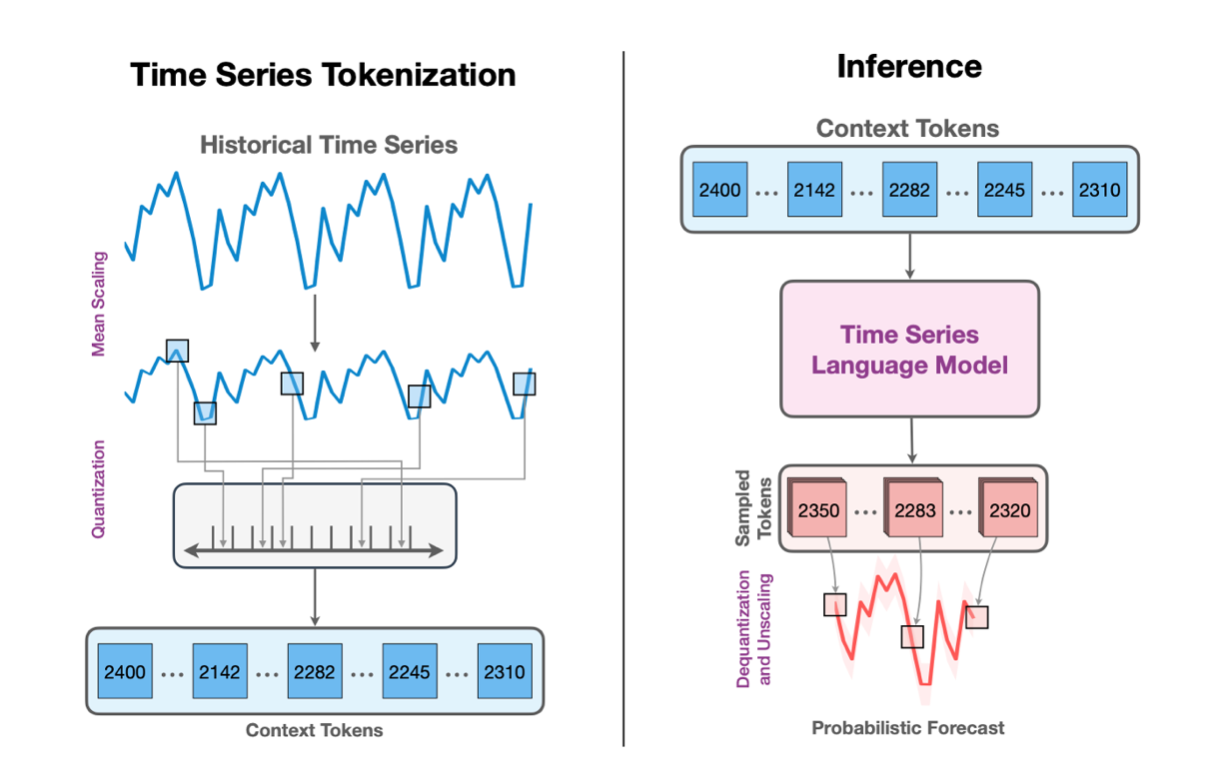
\includegraphics[width=0.8\textwidth]{chronos_inference.png}
  \caption{High-level Depiction of Inference of Chronos \parencite{ansari2024chronos}}.
  \label{chronosinference}
\end{figure}

\subsubsection{Available Methods and Capabilities}

The Chronos models are the five models in Table \ref{chronosmodels}. The only difference between them is the parameter sizes. \cite{ansari2024chronos} demonstrates that the bigger the model is, the better the result in their analysis. However, the largest model is significantly more computationally expensive. This is also why Chronos does not include larger models, as they would become impractical in real-world applications. 

\begin{table}[ht]
  \centering
  \caption{The Five Models of Chronos \parencite{ansari2024chronos}}
  \label{chronosmodels}
  \begin{tabular}{ccc} % Three centered columns
  \toprule
  \textbf{Model} & \textbf{Parameters} & \textbf{Based On} \\ 
  \midrule
  chronos-t5-tiny & 8M & t5-efficient-tiny \\ 
  chronos-t5-mini & 20M & t5-efficient-mini \\ 
  chronos-t5-small & 46M & t5-efficient-small \\ 
  chronos-t5-base & 200M & t5-efficient-base \\ 
  chronos-t5-large & 710M & t5-efficient-large \\ 
  \bottomrule
  \end{tabular}
\end{table}

\subsection{MOIRAI}

\cite{woo2024unified} introduced the \textit{\textbf{M}asker Enc\textbf{o}der-based Un\textbf{i}vers\textbf{a}l T\textbf{i}me Series Forecasting Transformer} (MOIRAI), a foundation model for time series forecasting, drawing inspiration from LLMs and vision transformers. Moirai utilizes a unified transformer-based architecture tailored for time series data. It is an open-source initiative developed collaboratively by Salesforce AI Research and the School of Computing and Information Systems at Singapore Management University.

\subsubsection{Model Architecture}

Moirai aims to handle time series data effectively by using a Masked Encoder architecture. This setup includes several input and output layers that can handle the different frequencies and types of data found in time series. These layers aim to help the model learn effectively from data that varies in speed and complexity.

\begin{figure}[htbp]
  \centering
  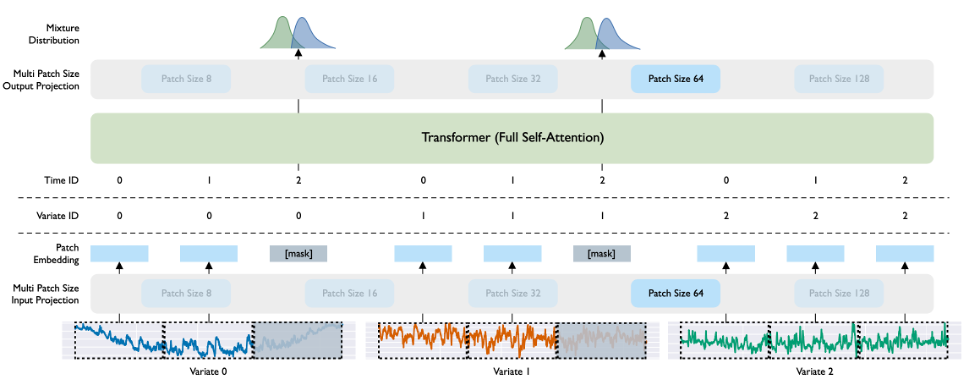
\includegraphics[width=0.8\textwidth]{moirari.png}
  \caption{High-level architecture of Moirai \parencite{woo2024unified}}.
  \label{moirari}
\end{figure}

Unlike typical transformers that handle single-dimension data, Moirai introduces \textit{Any-variate Attention} that treats all variates of a multivariate time series as a single sequence \parencite{woo2024unified}. This supposedly allows the model to process the full context of multivariate interactions. In the architecture, the basic transformer structure is maintained, but the data handling is adapted in an effort to meet the needs of universal time series forecasting.

\subsubsection{Training}

Moirai is trained on the Large-scale Open Time Series Archive (LOTSA), containing over 27 billion observations across various domains \parencite{woo2024unified}. 

\begin{table}[htbp]
  \centering
  \caption{Key Statistics Frequency and Domain of the LOTSA Data \parencite{woo2024unified}}
  \label{lotsdata}
  
  \tiny % Set the font size for the table to scriptsize
  % Redefine the X column type to center content
  \newcolumntype{C}{>{\centering\arraybackslash}X} % Centered X column type
  
  \begin{tabularx}{\textwidth}{C *{9}{C}}
  \toprule
   & \textbf{Energy} & \textbf{Transport} & \textbf{Climate} & \textbf{CloudOps} & \textbf{Web} & \textbf{Sales} & \textbf{Nature} & \textbf{Econ/Fin} & \textbf{Healthcare} \\
  \midrule
  \# Datasets & 30 & 23 & 6 & 3 & 3 & 6 & 5 & 23 & 6 \\
  \# Obs. & 16,358,600,896 & 4,900,453,419 & 4,188,011,890 & 1,518,268,292 & 428,082,373 & 197,834,339 & 28,547,647 & 24,919,596 & 1,594,281 \\
  \% & 59.17\% & 17.73\% & 15.15\% & 5.49\% & 1.55\% & 0.72\% & 0.09\% & 0.10\% & 0.01\% \\
  \bottomrule
  \end{tabularx}
  
  \vspace{1cm} % Spacing between the two tables
  
  \begin{tabularx}{\textwidth}{C *{8}{C}}
  \toprule
   & \textbf{Yearly} & \textbf{Quarterly} & \textbf{Monthly} & \textbf{Weekly} & \textbf{Daily} & \textbf{(Multi) Hourly} & \textbf{(Multi) Minute-level} & \textbf{(Multi) Second-level} \\
  \midrule
  \# Datasets & 4 & 5 & 10 & 7 & 21 & 31 & 25 & 2 \\
  \# Obs. & 873,297 & 2,312,027 & 11,040,648 & 18,481,871 & 709,017,118 & 19,875,993,973 & 7,013,949,430 & 14,794,369 \\
  \% & 0.003\% & 0.008\% & 0.040\% & 0.067\% & 2.565\% & 71.893\% & 25.370\% & 0.054\% \\
  \bottomrule
  \end{tabularx}
  
\end{table}
 
This diverse dataset helps Moirai learn a wide range of time series patterns, from economic indicators to climate data. Instead of just predicting single values, the model learns to predict the entire range of possible future values. This is done by training it to optimize a mix of parametric distributions, which prepares the model for both exact and probabilistic forecasts. The small model is trained for 100,000 steps, while the base and large models are trained for 1,000,000 steps. The training uses the Adam algorithm with weight decay (described in \ref{neuralnetworks}).

Moirai uses techniques like random sampling of context lengths and prediction horizons during training. This approach adds flexibility and robustness to the model's forecasting abilities.

However, there is a limitation to note for our thesis: Moirai has been trained on LOTSA, which includes data from the M3 Competition. This overlap will be considered since our thesis evaluates foundation models for time series using the M3 dataset.

\subsubsection{Approach to Time Series Forecasting}

Moirai does not generate point estimates when producing forecasts but predicts a distribution of future values. This is achieved by optimizing a mixture of parametric distributions, which allows the model to account for the inherent uncertainty in time series data \cite{woo2024unified}. By focusing on the distribution of possible future outcomes, Moirai provides forecasts that include both deterministic and probabilistic elements, reportedly making it versatile for various forecasting requirements.

\subsubsection{Available Methods and Capabilities}

The model comes in three versions to meet different computation and detail needs: Moirai-Small, Moirai-Base, and Moirai-Large. These versions have 14 million, 91 million, and 311 million parameters, respectively. Each version is designed to balance performance and computational efficiency, with the larger models offering more complexity and potentially higher accuracy in forecasting tasks across diverse datasets.

\subsection{Model Evaluation Metrics} \label{modelevaluationmetrics}

It is important to choose an appropriate metric when evaluating a model. Choosing these metrics is, unfortunately, not straightforward as there are many to choose from, and the different metrics serve different purposes. This subsection covers the ideas behind the evaluation metrics used in this thesis. 

The metrics aim to measure the forecast accuracy by summarizing, in different ways, the \textit{forecast errors}, where the forecast errors are the difference between observed values and the forecast. Errors do not refer to a mistake but rather the unpredictable part of an observation and can be written as $e_{T+h}$ for the training data $ \{{y_1,..,y_T\}}$ and the test data $\{{y_{(T+1)},y_{(T+2)},\ldots}\}$:

\begin{equation}
  e_{T+h} = y_{T+h} - \hat{y}_{T+h|T}
\end{equation}

It is important to note that the forecast errors are not the same as residuals. What differentiates forecast errors and residuals is: (1) residuals are calculated based on the observed values and the forecast on the training data, while forecast errors are calculated on test data, and (2) residuals are based on forecasting one time period ahead of each step while forecast errors can be based on the prediction of several future time periods \parencite{HyndmanForecasting2021}. 

Forecast errors can be further extended to find the \textit{percentage} error. This has the advantage of being unit-free and is therefore useful to compare forecast performance for different data sets \parencite{HyndmanForecasting2021}. The percentage error $p_t$ is given as:

\begin{equation}
  p_t = \frac{e_t}{y_t} \ast 100
  \label{percentageerror}
\end{equation}

This is to convert the forecast error $e_t$, the unit difference, to a percentage. Earlier, we defined $e_{T+h}$ to represent the forecast for $h$ periods ahead of time $T$. However, for simplicity and because the focus will shift solely to what would be the test data, we will use just time $t$ in subsequent discussions with $n$ samples of forecast errors. 

An alternative way of measuring is to base the calculation on \textit{relative errors}. This lets us compare the forecast error of a method with a benchmark. The relative error $r_t$ is: 

\begin{equation}
  r_t = \frac{e_t}{e_t^{\text{benchmark}}}
\end{equation}

In this formula, we find the relative error $r_t$ by dividing the forecast error $e_t$ by the forecast error of a benchmark method ${e_t^{\text{benchmark}}}$. This benchmark method is usually a \textit{random walk}, meaning the forecast is equal to the last observation \parencite[683]{HyndmanAccuracy2006}. 

\subsubsection{sMAPE}

The \textit{Symmetric Mean Absolute Percentage Error} (sMAPE) is a central metric to the M3 Competition. To understand sMAPE, starting with the related metric Mean Absolute Percentage Error (MAPE) is useful as it originates from this metric from which sMAPE originates. With the definition of $p_t$ from (\ref{percentageerror}), MAPE is given as: 

\begin{equation}
  \text{MAPE} = \frac{1}{n} \sum_{t=1}^{n} \left| p_t \right|
\end{equation}

As shown, MAPE calculates the mean of the percentage error \( p_t \) in absolute values. The MAPE has the disadvantage of becoming infinite or undefined when \( y_t \) is zero and extremely skewed when \( y_t \) is close to zero. Another disadvantage is that the MAPE puts a heavier penalty on positive errors than on negative errors, which led to the use of sMAPE, with a change in the denominator for MAPE to introduce “symmetry” \parencite[683]{HyndmanAccuracy2006}. The formula used in the competition with forecast error \( e_t \), observed values \( y_t \) and forecast \(\hat{y}_t\) is:

\begin{equation}
  \text{sMAPE} = \frac{1}{n} \sum_{t=1}^{n} \frac{\left| e_t \right| \ast 100}{( y_t + \hat{y}_t ) / 2}
  = \frac{1}{n} \sum_{t=1}^{n} \frac{\left| e_t \right| \ast 200}{( y_t + \hat{y}_t )}
\end{equation}

The denominator, ${\left| y_t \right| + \left| \hat{y}_t \right|}$, aims to add symmetry by balancing the error in relation to the size of both the observed and forecasted values. This means that the forecast error in an absolute value will be divided by the average of the observed and forecasted values to create a more stable error metric. 

With sMAPE, problems with small values for \( y_t \) are less severe as the forecast value \( \hat{y}_t \) is added to the denominator. However, when \( y_t \) is close to zero, \( \hat{y}_t \) is also likely to be close to zero if the forecast is accurate \parencite[683]{HyndmanAccuracy2006}. This means the measure can still involve a division by a number close to zero, potentially making it unstable. Furthermore, sMAPE can take negative values, as the denominator is the average of the forecast and actual values, not their absolute values, making it not truly a metric of “absolute” percentage errors \parencite{HyndmanForecasting2021}. The denominator, however, is defined in absolute values for the M4-Competition \parencite{Makridakis2019}. Additionally, the penalty for a low value of \( \frac{\left| e_t \right|}{( y_t + \hat{y}_t ) / 2} \) is more costly compared to a higher value with the same \( y_t \). This implies that a model consistently underestimating is penalized less severely than one that overestimates by the same absolute value, making the metric not as symmetric as its name might suggest \parencite{GoodwinSmape1999}.

The sMAPE is also used to determine the \textbf{Average Ranking} in the competition, which is the average ranking of the sMAPE for each method for each forecast horizon \parencite{MAKRIDAKIS2000}.

Although this metric is central in the M3 Competition and is widely used, \cite{HyndmanAccuracy2006} argues that sMAPE should be avoided due to the mentioned issues. We will, therefore, not use this metric to the extent done in the M3 Competition to evaluate our findings. 

\subsubsection{MdAPE}

\textit{Median Absolute Percentage Error} (MdAPE) is one of the most used metrics based on percentage errors. It is given as: 

\begin{equation}
  \text{MdAPE} = \text{median} \left( \left| p_t \right| \right)
\end{equation}

This rather simple metric returns the median percentage error $p_t$ in absolute values. The MdAPE has the advantage, as mentioned earlier, of being metric based on percentage error. However, it has the same disadvantages as discussed for MAPE with being infinite or undefined for $y_t = 0$, being skewed when close to zero and has asymmetry in penalties between positive and negative errors \parencite[683]{HyndmanAccuracy2006}. 

\subsubsection{MdRAE}

The \textit{Median Relative Absolute Error} (MdRAE) is similar to MdAPE, but the percentage error $p_t$ is exchanged for the relative error $r_t$:

\begin{equation}
  \text{MdRAE} = \text{median} \left( \left| r_t \right| \right)
\end{equation}

The MdRAE will, as the name reveals, be the median of the relative errors in absolute values. As mentioned, we find the relative error $r_t$ by comparing two methods, often a random walk as the benchmark. In the M3-Competition, the seasonal naïve method is used as the benchmark, which is a variation of a random walk as covered in Section (\ref{naivesection}), Naïve Forecasting. However, this metric also has drawbacks. When the relative error to the benchmark ${e_t^{\text{benchmark}}}$ is close to zero, it introduces an instability, as with sMAPE, which is not ideal \parencite[683]{HyndmanAccuracy2006}. 

\subsubsection{RMSE}

The \textit{Root Mean Square Error} (RMSE) is one of the most used scale-dependent accuracy metrics. It is scale dependent as it is only based on the forecast error $e_t$ and is therefore incompatible for comparisons between series with different units \parencite{HyndmanForecasting2021}. The RMSE is calculated as: 

\begin{equation}
  \text{RMSE} = \sqrt{\frac{1}{n} \sum_{t=1}^{n} e_t^2}
\end{equation}

In the RMSE, all forecast errors $e_t$ are squared, returning a positive number. The square root of the average of these numbers will be the value for this metric. As it sums the squared forecast errors, larger errors will have a bigger impact on the result than other metrics. It is also more sensitive to fluctuations in the forecast errors, in absolute values, especially if the errors are inconsistent \parencite{Willmott2005}. This means that if there are big swings in how much the predictions are off, the RMSE will penalize this heavier than other metrics. 

\subsubsection{MASE}

\cite{HyndmanAccuracy2006} proposes to use scaled error in an accuracy metric \textit{Mean Absolute Scaled Error} (MASE) as a better alternative than the previous metrics. As such, this metric will be central to our evaluation. The scaled error $q_t$ is defined when benchmarking against seasonal naïve method as: 

\begin{equation}
  q_t = \frac{e_t}{\frac{1}{n-m} \sum_{t=m+1}^{n} \left| y_t - y_{t-m} \right|}
\end{equation}

This is to make the metric independent of the scale of the data. The denominator represents the average error of a naïve one-step ahead prediction $y_t-y_{\left(t-1\right)}$ in absolute values. This means that the scaled error $q_t$ measures forecast error normalized against the average of the forecast errors a naïve method would have. To then obtain the MASE, we simply average these scaled errors $q_t$ in absolute values over the forecast period n:

\begin{equation}
  \text{MASE} = \frac{1}{n} \sum_{t=1}^{n} \left| q_t \right|
\end{equation}

While MASE might initially seem complex, it is a user-friendly indicator of forecast accuracy: a score below 1 indicates better performance than the naive benchmark, around 1 means similar performance, and above 1 suggests poorer performance \parencite[684--685]{HyndmanAccuracy2006}.




% \begin{center}
%   \section{Methodology}
% \end{center}
\newpage
{\centering \section{Methodology} \par}

\subsection{Introduction}

In this section, we outline the methodology used to evaluate the performance of foundation models in zero-shot forecasting with the M3-Competition dataset. First, we describe the M3-Competition dataset, which includes a diverse collection of time series data across yearly, quarterly, and monthly frequencies. This dataset is widely used and provides robust benchmarks for comparison. Next, we detail the evaluation process. We use the Mean Absolute Scaled Error (MASE) score to measure forecast accuracy, comparing the foundation models to the Naïve2 benchmark. Finally, we explain how the foundation models—Chronos, TimeGPT, and Moirai—were used in this study. We describe their setup for zero-shot forecasting, the data preprocessing steps, and the systematic recording of results for analysis. Figure \ref{methodology} shows a high-level depiction of the methodology of this thesis. 


\begin{figure}[htbp]
  \centering
  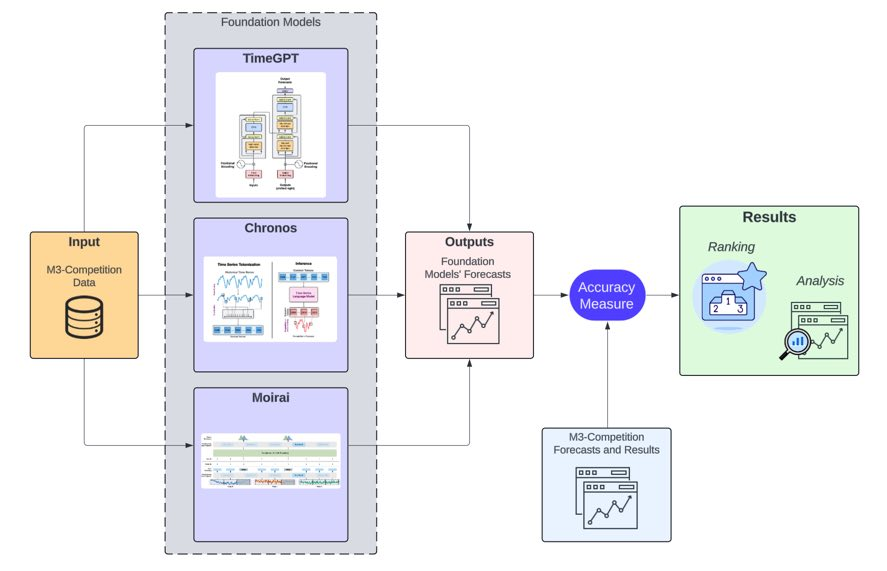
\includegraphics[width=0.8\textwidth]{method_fig.png}
  \caption{Illustration of the methodology used in this thesis.}
  \label{methodology}
\end{figure}

\subsection{Competition Selection}


In selecting an appropriate time series forecasting competition for zero-shot forecasting, several factors were considered to ensure the chosen competition aligned with our research goals. A primary criterion was the transparency of the competition's processes. It was essential that the methodology behind the results, particularly how they were derived and evaluated, was openly available and documented. This transparency was fundamental for several reasons. First, having access to both training data and the forecasted outputs from other methods was crucial for a meaningful evaluation. Second, the documentation of the methods used influences the credibility and trustworthiness of the results. Lastly, comprehensive documentation supports not only the internal validity of our findings but also reflects on the competition's academic integrity and reputation. 

We sought a competition recognized for its academic rigor and respect within the field, attracting participants with a robust knowledge base, which would reinforce the relevance and suitability of our choice.

Moreover, while managing practical considerations, we acknowledged certain constraints and necessities. TimeGPT was supported by a grant of $2,000$ USD in API credits from Nixtla. For instance, selecting a competition requiring extensive training data could disadvantage the model if our resources were insufficient to handle the volume. Additionally, the foundation models evaluated in our study require substantial computing power, which increases with the size of the dataset. We also aimed to avoid competitions where unique data engineering techniques or specialized data sources could introduce unfair assessment, such as in the M5-Competition competition, where these factors are significant. 

Finally, the data needed to contain diverse time series attributes. Evaluating the generalizability of the foundation models required analyzing their performance across various time frequencies. This approach ensured an assessment of the model's ability to adapt and forecast effectively over differing time frequencies, providing a robust indication of its versatility and applicability in real-world scenarios.

\subsubsection{The M3 Competition}

The M3-Competition is part of a series of forecasting competitions spanning back to 1982 when Spyros Makridakis first introduced the competition \parencite{IIF}. There have been a total of 5 competitions where different forecasting methods have been compared and evaluated, where the latest, the M5-Competition, took place in 2020 \parencite{Makridakis2019}. We decided to evaluate the foundation models in the M3-Competition as this best aligned with our abovementioned requirements.

The competition uses real-world data from various fields like finance, demographics, and economics. Its academic nature ensures detailed documentation and scholarly discussion, providing a solid basis for evaluation. Importantly, the dataset is simple, including only the target forecast values and their time intervals, with no extra features. It includes different time frequencies—yearly, quarterly, and monthly—giving a broad perspective on zero-shot forecasting. Additionally, the M3-Competition uses a standard evaluation framework with pre-defined metrics, ensuring consistent and comparable results. These features make the M3-Competition an excellent platform to evaluate our foundation models against established forecasting methods.

\paragraph{Methods Used in the M3-Competition}

The M3-Competition saw 24 different forecasting methods used. The authors have categorized the methods into six categories, namely Naïve/Simple, Explicit Trend Models, Decomposition, ARIMA/ARARMA model, Expert Systems, and Neural Networks. All categories and methods are shown in Table \ref{methods_used_m3} along with their respective approach to forecasting. Descriptions of the methods and the competitors' names are found in \hyperref[appendix_a]{Appendix A}.

\begin{table}[htbp]
  \centering
  \begin{threeparttable}
  \caption{Forecasting Methods Used in the M3-Competition}
  \label{methods_used_m3}
  \begin{tabularx}{\textwidth}{@{}Xll@{}} % Using X for the first column to handle text overflow nicely
  \toprule
  \textbf{Category} & \textbf{Model} & \textbf{Forecasting Approach} \\
  \midrule
  \multirow{5}{*}{Naïve/Simple} & NAÏVE2 & Random Walk for seasonally adjusted data \\
  & SINGLE\tnote{*} & Single Exponential Smoothing \\
  & HOLT & Holt’s Linear Method \\
  & ROBUST-Trend & Holt’s Linear Method \\
  & WINTER & Holt-Winter’s Seasonal Method \\
  \addlinespace % Adding a small vertical space between groups
  \hline
  \multirow{2}{*}{Explicit Trend Models} & DAMPEN & Holt’s Linear Method with Dampening \\
  & PP-Autocast & Holt’s Linear Method with Dampening \\
  \addlinespace
  \multirow{2}{*}{Decomposition} & THETAsm & Hybrid of approaches \\
  & COMB S-H-D & Hybrid of approaches \\
  \addlinespace
  \hline
  \multirow{8}{*}{ARIMA/ARARMA Models} & THETA & THETA \\
  & B-J Auto & ARIMA \\
  & AutoBox 1 & ARIMA \\
  & AutoBox 2 & ARIMA \\
  & AutoBox 3 & ARIMA \\
  & AAM 1\tnote{*} & ARIMA \\
  & AAM 2\tnote{*} & ARIMA \\
  & ARARMA & ARARMA \\
  \addlinespace
  \hline
  \multirow{6}{*}{Expert Systems} & ForecastPro & Choose between several \\
  & SMARTFCS & Choose between several \\
  & RBF & Choose between several \\
  & Flors-Pearc1 & Choose between several \\
  & Flors-Pearc2 & Choose between several \\
  & ForcX & Choose between several \\
  \addlinespace
  \hline
  Neural Networks & Auto-ANN & Deep Learning \\
  \bottomrule
  \end{tabularx}
  \begin{tablenotes}
  \small
  \item[*] The models marked with a star are excluded from our analysis. The AAM 1 and AAM 2 models are excluded as they lack forecasts for yearly data. The Single Exponential Smoothing model SINGLE is also excluded due to data quality concerns.
  \end{tablenotes}
  \end{threeparttable}
  \end{table}

\paragraph{Accuracy Metrics in the M3-Competition}

\cite{MAKRIDAKIS2000} use five different accuracy metrics to evaluate the models in the M3-Competition. However, due to the disadvantages of these metrics outlined in section (\ref{modelevaluationmetrics}), they will not be central to our evaluation. Nonetheless, we report results for sMAPE, MdAPE and MdRAE as per \cite{MAKRIDAKIS2000} in \hyperref[appendix_c]{Appendix C}. The accuracy metrics in the M3 Competition are described in Table \ref{forecasting_metrics_m3}. 

\begin{table}[htbp]
  \centering
  \caption{Accuracy Metrics Used in the M3-Competition}
  \label{forecasting_metrics_m3}
  \begin{tabularx}{\textwidth}{lX}  % First column left aligned, second column justified and flexible width
  \toprule
  \textbf{Metric}                                           & \textbf{Description} \\
  \midrule
  sMAPE (Symmetric Mean Absolute Percentage Error)          & Averages the absolute percentage error between predicted and actual values. \\
  \hline
  Average Ranking                                           & Average ranking with sMAPE for each method for each horizon. \\
  \hline
  Percentage Better                                         & Percentage of times that a given method has smaller forecasting errors than another method. \\
  \hline
  MdAPE (Median Absolute Percentage Error)                  & Median of percentage errors between forecasts and actual values. \\
  \hline
  MdRAE (Median Relative Absolute Error)                    & Compares median of absolute errors between a forecast and a benchmark forecast (NAÏVE2). \\
  \bottomrule
  \end{tabularx}
\end{table}

\subsection{Evaluation}
To evaluate the foundation models, we compared their performance against 20 previously assessed methods in the M3-Competition. The evaluation proceeded in two phases. Initially, we created a leaderboard that ranks the models based on their overall performance. This leaderboard provides a clear, comparative overview of how each model performs across all data included in the competition.

In the subsequent phase, we conducted a more detailed analysis of the foundation models’ performance. This deeper examination reviewed their results across different categories of data and time frequencies, as done in the M3-Competition. The aim is not only to discover where foundation models stand in the overall rankings but also to understand their strengths and weaknesses in specific forecasting scenarios compared to the traditional methods. This approach lets us provide both a broad overview and a detailed look at how foundation models perform in the field of zero-shot time series forecasting.

\subsubsection{Evaluation Metrics}

To assess how effective the foundation models are, we used the evaluation metrics described in section (\ref{modelevaluationmetrics}). We deviated from the methodology of \cite{MAKRIDAKIS2000} by primarily focusing on MASE (Mean Absolute Scaled Error) instead of sMAPE (symmetric Mean Absolute Percentage Error). This choice was informed by the recognition that sMAPE, despite its central role in the original competition's evaluation, has acknowledged limitations. \cite{HyndmanAccuracy2006} notably advise against using sMAPE due to these concerns.

However, to provide some consistency with the M3-Competition, we present our results with sMAPE as metric in Table \ref{smape_scores_table} and \hyperref[appendix_c]{Appendix C}, mirroring the reporting style of \cite{MAKRIDAKIS2000}. Here sMAPE is defined in absolute values for the numerator and denominator as done by \cite{Makridakis2019}.

\subsubsection{Benchmark Model}

As relative and scaled errors used in MdRAE and MASE require a model performance as a comparison, we will use the Naïve2 method as a benchmark, consistent with the work of \cite{MAKRIDAKIS2000}. The Naïve2 method extends the simplicity of the naïve forecasting model by adjusting for seasonality, providing a baseline that accounts for systematic, seasonal variations in the data. The Naïve2 is defined as:

\begin{equation}
  F_{\left(t+i\right)}=X_t^\ast\left(S_j\right)
\end{equation}

The Naïve2 creates a forecast $F_{\left(t+i\right)}$ by multiplying a seasonally adjusted time series $X_t^\ast$ with a seasonal component $S_j$. The seasonality is removed from the time series as $X_t^\ast = \frac{X_t}{S_j}$. The seasonal component $S_j$ is computed using classical decomposition method for $j$ periods, which can be quarterly or monthly. This is done for forecast index $i$, which goes to 6 for yearly data, 8 for quarterly, and 18 for monthly. 

\subsubsection{Leaderboard}

In the M3 Competition, \cite{MAKRIDAKIS2000} chose not to rank the 24 competing forecasting methods. They understood that forecasting is complex, and a single ranking might not accurately show how different methods perform across various categories and time frequencies. This approach highlights the importance of context and specific conditions when evaluating forecasting methods.

Despite these considerations, we believe there is value in providing a straightforward overview of how each method performs. Therefore, we have decided to include a leaderboard in our analysis. This leaderboard will rank the methods based on the median MASE. The intention is not to declare a definitive champion method but rather to offer a look at overall performance, especially regarding the foundation models.

We understand and acknowledge the limitations of a simple ranking system. Subsequent sections of our evaluation explore how each method performs across different data categories and time frequencies. This layered approach provides a broad overview and a detailed evaluation.


\subsubsection{Time Frequencies}

Given that the M3-Competition includes yearly, quarterly, and monthly data, it is important to consider how the models perform within these frequencies. This analysis helps identify both the strengths and potential shortcomings of the foundation models. To achieve this, we calculated the median MASE for each time frequency subset to determine if there are differences in outcomes. Additionally, we examine how the MASE scores evolve throughout the forecast horizon for these subsets. Finally, we analyze the distributions within each subset to identify any patterns or developments.

\subsubsection{Categories}

Similar to our analysis of time frequencies, investigating how the models perform across each data category helps us determine if there are specific categories where foundation models excel or fall short. We examined the median MASE scores for each category to evaluate the performance variations. Additionally, we present both mean and median MASE scores for each time frequency and category to offer a comprehensive overview of performance at the most granular level available in the M3-Competition dataset. 

\subsubsection{Comparison Against Benchmark}

We dedicate a section to better understanding the foundation models' performance compared to the benchmark. As the MASE scores are already scaled to the benchmark performance, we deviate from MASE for simplicity.

First, we calculate the \textit{Percentage Better}, which represents the percentage of times each foundation model achieves a MASE score lower than 1, indicating performance superior to the Naïve2 benchmark. This metric does not consider the magnitude by which models outperform the benchmark, only how frequently they do. Secondly, we draw inspiration from \cite{MAKRIDAKIS2000} to investigate how a selection of models performs across different forecasting horizons using average sMAPE scores against the Naïve2 benchmark. 


\subsection{Statistictical Tests}

Statistical testing of the results is fundamental to validate the accuracy and reliability of our findings. To achieve this, we will employ multiple methods. First, we will visualize the results by displaying the distribution of median MASE scores obtained through bootstrap sampling. However, resampling methods do not produce independent values for the evaluation metrics and might lead to underestimating the variance in the performances.

\cite{Koning2005} notes the importance of statistical testing for evaluating forecast accuracy, as relying on descriptive statistics can lead to inaccurate conclusions. We follow a methodology proposed by \cite{Rainio2024} for statistical testing in comparing models. First, we want to investigate if the performance of the three foundation models is significantly different. For this comparison, we test using the \textit{Friedman’s test}. The null hypothesis here is that the differences in model performances are statistically significant. This test has been performed in its original notation. Secondly, we want to test if the amount of variance the foundation models produce is similar. We use the \textit{Levene’s test} to test the null hypothesis that the variances from the model performances are equal. Additionally, we use the \textit{Wilcoxon Signed-Rank test} to test for significant differences between potentially interesting pairs of models. This has the same objective as the Friedman’s test, but it is for assessing between any two models rather than a group of models. 


These tests have the advantage of not being sensitive to the choice of evaluation metric and can be used for data that is not normally distributed. We used the \textbf{scipy.stats} functions \texttt{friedmanchisquare, levene, and wilcoxon}.

\subsection{Implementation - TimeGPT}

This section covers how the results for TimeGPT were obtained, meaning how the forecasts were made and what data was given to the model. In addition, it is important to mention that it is not entirely reproducible as TimeGPT requires an \textit{application programming interface} (API) key. Nonetheless, all the data and scripts are uploaded to \href{https://github.com/tom-alten/Outsmarting-Time/}{GitHub}, meaning interested parties may perform any complimentary analyses.  

\subsubsection{Access}

Using the model requires an API key that may be obtained by request to Nixtla. We were fortunate enough to receive 2,000 USD in credits for academic purposes. 

\subsubsection{Reproducibility}

Since TimeGPT is proprietary and not publicly available, our study cannot be directly replicated by others, which may impact the perceived robustness of our findings. To mitigate this limitation, we have taken steps to enhance the reproducibility of our work as much as possible. Additionally, we have uploaded all the data files utilized in our study to this repository, including the outputs generated by TimeGPT. We used the first release of the model, and forecasts were produced on 18.04.2024. This approach aims to provide transparency and assist others in understanding and verifying our research processes and results.

\subsubsection{API Data Integration}

Due to its proprietary nature, TimeGPT is not meant to be hosted locally on personal hardware but is accessed through an API. The model's complexity and the requirement to keep its weights inaccessible necessitate this remote operation. To interact with TimeGPT, data must be transmitted to the model via the API to generate forecasts.

To manage this process efficiently, data, once prepared, is fed into the model using a for loop. This loop is structured to pace the data input, ensuring it adheres to the API's rate limits. Each batch of data sent receives forecasts, which are then stored along with the corresponding series identifiers. All the resulting data is saved using Apache Parquet format. Parquet was chosen because of its quick read capabilities and its reliable preservation of data types, which helped maintain uniformity in our data processing workflow.

\subsection{Implementation - Chronos \& Moirai}

This section describes the technical approach employed to generate forecasts using the MOIRAI and Chronos models, focusing on data preparation, model configuration, and forecast generation. It is important to note that although our configuration was comprehensive, simplicity was a key goal. Our intuition is that the main advantage of a foundation model is its ability to generalize without requiring extensive configurations. Therefore, we limited ourselves to essential adjustments, aiming to assess the model’s effectiveness in zero-shot forecasting. 

\subsubsection{Data Preparation}

The forecasting process started with loading the time series data from a preprocessed Parquet file. Each time series is uniquely identified and isolated from the larger dataset to ensure the integrity and independence of each forecasting instance. Unlike Chronos, Moirai cannot handle data in the commonly used Pandas format directly and requires the data in the format of GluonTS, a Python library for probabilistic time series modeling in Python. 

\subsubsection{Model Configuration}

When configuring both the Moirai and Chronos models, we opted for the "base" model size. This choice provided a balance between computational efficiency and predictive performance suitable for our hardware's constraints. While the larger variants of these models could have provided increased accuracy, their demands on computational resources and memory were too intensive for our hardware.

Consistent with our goal of simplicity, we aimed to minimize complexity in setting up the models. Our configurations closely followed the default settings recommended in their respective GitHub repositories, ensuring we could assess each model's zero-shot forecasting abilities without unnecessary modifications. 

\subsubsection{Forecast Generation and Storage}

Forecasts were generated by iterating through each unique series in the dataset. For each series, the model considers only the first $N-NF$ records for training, where $N$ is the total number of observations in the series, and $NF$ is the number designated for forecasting. This approach mirrors the training-test split commonly used in time series analysis but is adapted here for the M3-Competition.

Both models output a set of probabilistic distributions for future values. These distributions were processed to extract the median forecast at each time step, giving a central tendency measure that is robust to outliers and extreme values. This was done because we focus on point forecasts rather than on distributions.

The forecasts generated for each series were compiled into a single DataFrame. This DataFrame was systematically updated with each batch of forecasts while maintaining a record of all predictions made during the session. Once all forecasts were generated and recorded, the DataFrame was saved as a Parquet file for further analysis.


% \begin{center}
%   \section{Data}
% \end{center}
\newpage
{\centering \section{Data} \par}

\subsection{Data Collection}

The dataset used in our thesis was obtained from the International Institute of Forecasters' official website \parencite{IIF}. This dataset encompasses the actual data and the results of the M3-Competition, detailed in \parencite{MAKRIDAKIS2000}. 

\subsection{Data Quality}

The dataset was subjected to rigorous quality checks to identify any potential issues. The data was reliable during our exploratory analysis and cleaning process, with no significant quality concerns. However, we did encounter an inconsistency concerning the dataset's values: it was noted in \cite{MAKRIDAKIS2000} that all values were supposed to be non-negative, aligning with the requirements of using sMAPE as an accuracy metric. Despite this, we discovered one instance where a value did not meet this criterion. We decided to retain this inconsistency in the dataset to maintain consistency with the M3-Competition's methodology and ensure that our results could be comparable with those from the competition.

\subsection{Data Description} \label{data_description}

The dataset used in this thesis consists of real-world data from various domains, though specific details about the data's origins are not provided. This dataset includes time series data that varies in length depending on its time frequency: yearly series require at least 14 observations, quarterly series need at least 16, and monthly series must have a minimum of 48 observations as per \cite{MAKRIDAKIS2000}. As previously discussed, a desirable feature of our purpose was the exclusion of exogenous variables, a requirement fulfilled by this dataset. 

Time series with intervals labeled as "other" are not included in our analysis. This exclusion is necessary because our foundation models require a structured timestamp to produce forecasts. Including these series could lead to unreliable forecasting results, as the results would be more dependent on the frequency we assigned, affecting their validity. 

One frequently encountered challenge in time series is managing outliers, which our dataset contains. This allows us to evaluate how well the foundation models handle real-world data scenarios. The boxplots (\ref{boxplot_data_distribution}) show that variations do exist while the overall distribution is fairly consistent across different categories. 

\begin{figure}[htbp]
  \centering
  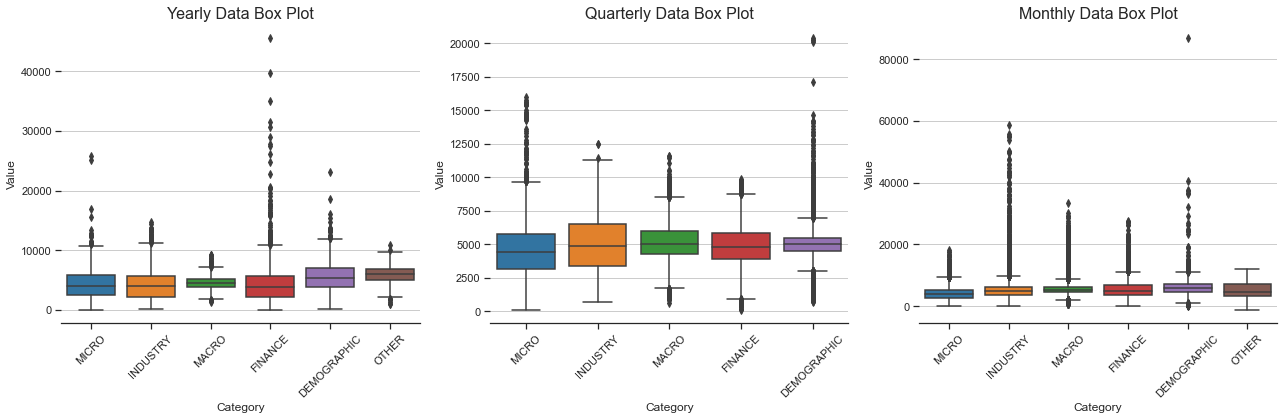
\includegraphics[width=0.8\textwidth]{real_boxplot_data_descr.png}
  \caption{Boxplots of categories across the different time frequencies.}
  \label{boxplot_data_distribution}
\end{figure}

Specifically, some categories are more susceptible to outliers and demonstrate a higher level of skewness in their data distribution. The categories "Demographic" and "Finance" stand out as having more outliers than the other categories.

The table of summary statistics (\ref{summary_statistics}) for each category, broken down by frequency (monthly, quarterly, and yearly), reveals interesting aspects of our data. For example, some categories, particularly within the monthly frequency, show significant variance between their minimum and maximum values, indicative of potential outliers. The skewness, inferred from the spread between the $25th$ and $75th$ quantiles, suggests a deviation from a normal distribution in several categories, which is affirmed by histogram plots in \hyperref[appendix_b]{Appendix B}. 

\begin{table}[htbp]
  \centering
  \caption{Summary Statistics of the M3-Competition Dataset}
  \label{summary_statistics}
  \begin{tabular}{llrrrrr}
  \toprule
  \textbf{Frequency} & \textbf{Category} & \textbf{Min} & \textbf{Lower Quartile} & \textbf{Mean} & \textbf{Upper Quartile} & \textbf{Max} \\
  \midrule
  \multirow{6}{*}{Monthly} & DEMOGRAPHIC & 120.00 & 4,706.00 & 5,971.10 & 7,257.25 & 86,730.00 \\
                           & FINANCE     & 10.00  & 3,643.65 & 5,265.75 & 6,663.05 & 27,505.00 \\
                           & INDUSTRY    & 90.00  & 3,600.00 & 4,966.40 & 6,050.00 & 58,676.00 \\
                           & MACRO       & 635.00 & 4,545.00 & 5,568.18 & 6,212.38 & 33,350.00 \\
                           & MICRO       & 100.00 & 2,600.00 & 4,082.09 & 5,260.00 & 18,100.00 \\
                           & OTHER       & -1,200.00 & 3,160.00 & 5,149.64 & 7,001.90 & 11,855.20 \\
  \midrule
  \multirow{5}{*}{Quarterly} & DEMOGRAPHIC & 720.00 & 4,524.12 & 5,114.14 & 5,507.55 & 20,375.00 \\
                             & FINANCE     & 121.00 & 3,875.00 & 4,871.71 & 5,820.82 & 9,903.33 \\
                             & INDUSTRY    & 680.00 & 3,350.00 & 5,055.66 & 6,541.59 & 12,465.00 \\
                             & MACRO       & 650.00 & 4,267.68 & 5,178.98 & 5,976.80 & 11,601.60 \\
                             & MICRO       & 126.00 & 3,141.00 & 4,589.06 & 5,764.40 & 15,973.00 \\
  \midrule
  \multirow{6}{*}{Yearly} & DEMOGRAPHIC & 170.80 & 3,832.00 & 5,456.84 & 7,052.70 & 23,103.30 \\
                          & FINANCE     & 30.00  & 2,175.90 & 4,352.19 & 5,642.04 & 45,525.66 \\
                          & INDUSTRY    & 83.10  & 2,144.75 & 4,118.87 & 5,764.00 & 14,710.40 \\
                          & MACRO       & 1,334.00 & 3,874.75 & 4,595.86 & 5,226.50 & 9,268.50 \\
                          & MICRO       & 48.00  & 2,432.24 & 4,304.06 & 5,855.75 & 25,805.00 \\
                          & OTHER       & 1,000.00 & 4,947.50 & 5,835.10 & 6,920.00 & 10,900.00 \\
  \bottomrule
  \end{tabular}
\end{table}

As mentioned in (\ref{timeseries}), stationarity concerns the trend and seasonality of the data. To address this, \textit{Augmented Dickey Fuller} (ADF) tests were performed for each time series. ADF tests have the null hypothesis that the series are non-stationary \parencite{HyndmanForecasting2021}. In our case, this is true for 2,341 of the 2829 unique time series. This high incidence of non-stationarity further confirms that it is representable as real-world data. 

\subsection{Data Preparation}

The M3-Competition dataset was supplied in an Excel file that included actual values as well as forecasts from various models. It had to be adapted to get the data ready for analysis with foundation models. First, we reshaped the dataset from a wide to a long format, which made working with DateTime values and merging operations more straightforward. During this transformation, careful attention was paid to the management of identifier columns to ensure the accuracy and consistency of the data.

One of the benefits of the M3-Competition dataset is that it does not contain exogenous variables, so there was no need for the extra steps of feature engineering or selection. This streamlined the preprocessing work. For greater efficiency in our analysis, we converted all data files to the Apache Parquet format.

\subsection{Data Limitations}
In the foundation models we evaluate, there is a difference in the time frequency of the data they are trained on. For instance, Moirai training utilized the LOTSA dataset, in which a mere 0.003\% represents yearly data. For the models we utilize, the bulk of the training data for these models, except for TimeGPT, where the training data is proprietary, consists mainly of hourly data. Although these models are architected to perform zero-shot forecasting across various frequencies, the amount of hourly data in their training raises questions about their effectiveness at different frequencies. This aspect requires closer examination in the results section, especially regarding its impact on model performance with yearly data. Moreover, the M3 dataset does not extend to time frequencies lower than monthly, so it does not thoroughly test the capabilities to handle the time frequency most represented in their training data.

% \begin{center}
%   \section{Results}
% \end{center}
\newpage
{\centering \section{Results} \par}

In this section, we present the results of our investigation into the performance of the three foundation models in the M3-Competition. Our research focuses on these models' performance in zero-shot forecasting, aiming to highlight their strengths, limitations, and comparative performance for the dataset. 

\subsection{Competition Results}

Before evaluating model performance, we provide an overview of the median MASE scores obtained for the foundation models in our evaluation. The median MASE scores show a contrast in performance by the foundation models. THETA is, as mentioned in the original competition, the model to beat for the foundation models to be crowned as superior models. While Chronos is showing a promising result and emerges as a potential contender, TimeGPT and Moirai fall far behind, displaying accuracy levels comparable to the Naive2 benchmark of MASE equal to one. 

\begin{figure}[htbp]
  \centering
  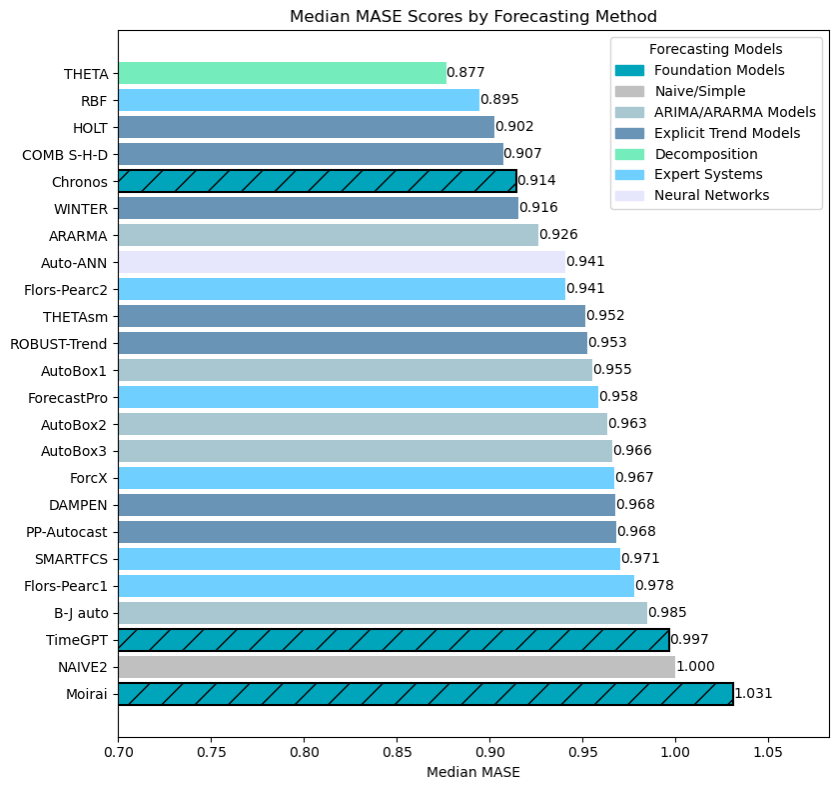
\includegraphics[width=0.8\textwidth]{median_mase_overall.png}
  \caption{Median MASE scores for all models in the M3-Competition.}
  \label{median_mase_scores}
\end{figure}

The notched boxplot in (\ref{boxplot_mase_scores}) shows the distribution of the MASE scores for a selection of competitors in our evaluation with the median as a red line. The selection consists of the top-performing models in the M3-Competition and the foundation models. This showcases that the greater part of the interquartile range (IQR) for TimeGPT and Moirai falls over the benchmark of a MASE score equal to one.

\begin{figure}[htbp]
  \centering
  \includegraphics[width=0.8\textwidth]{boxplot_mase_results.png}
  \caption{Boxplot of MASE scores for selected models in the M3-Competition.}
  \label{boxplot_mase_scores}
  \caption*{Note: The outliers for the MASE scores are excluded as all the models have significant outliers in MASE scores which makes the plot unreadable.}
\end{figure}

\subsubsection{Leaderboard Position}

As mentioned, the M3-Competition do not provide a leaderboard for its participants in the competition. We, however, present our ranking of the models here to provide a clear overview of model performance. Our findings rank the models as shown in Table (\ref{mase_results_complete}), with THETA emerging as the top model.

\begin{table}[htbp]
  \centering
  \caption{MASE results in the M3-Competition}
  \label{mase_results_complete}
  \resizebox{\textwidth}{!}{%
  \begin{tabular}{lllllll}
  \textbf{Rank} & \textbf{Method} & \textbf{Category} & \textbf{Median Score*} & \textbf{Mean Score} & \textbf{Lower Quartile} & \textbf{Upper Quartile} \\ \hline
  1 & THETA & Decomposition & 0.88 & 1.02 & 0.63 & 1.10 \\
  2 & RBF & Expert Systems & 0.89 & 1.12 & 0.60 & 1.23 \\
  3 & HOLT & Explicit Trend & 0.90 & 1.26 & 0.59 & 1.28 \\
  4 & COMB S-H-D & Explicit Trend & 0.91 & 1.01 & 0.68 & 1.08 \\
  \textbf{5} & \textbf{Chronos} & \textbf{Foundation Model} & \textbf{0.91} & \textbf{1.05} & \textbf{0.66} & \textbf{1.18} \\
  6 & WINTER & Explicit Trend & 0.92 & 1.26 & 0.63 & 1.23 \\
  7 & ARARMA & ARIMA/ARARMA & 0.93 & 1.26 & 0.59 & 1.36 \\
  8 & Auto-ANN & Neural Networks & 0.94 & 1.17 & 0.67 & 1.26 \\
  9 & Flors-Pearc2 & Expert Systems & 0.94 & 1.17 & 0.68 & 1.24 \\
  10 & THETAsm & Explicit Trend & 0.95 & 1.01 & 0.80 & 1.11 \\
  11 & ROBUST-Trend & Explicit Trend & 0.95 & 1.16 & 0.62 & 1.36 \\
  12 & AutoBox1 & ARIMA/ARARMA & 0.96 & 1.33 & 0.62 & 1.37 \\
  13 & ForecastPro & Expert Systems & 0.96 & 1.10 & 0.63 & 1.08 \\
  14 & AutoBox2 & ARIMA/ARARMA & 0.96 & 1.31 & 0.63 & 1.23 \\
  15 & AutoBox3 & ARIMA/ARARMA & 0.97 & 1.27 & 0.62 & 1.38 \\
  16 & ForcX & Expert Systems & 0.97 & 1.06 & 0.67 & 1.10 \\
  17 & DAMPEN & Explicit Trend & 0.97 & 1.06 & 0.71 & 1.08 \\
  18 & PP-Autocast & Explicit Trend & 0.97 & 1.11 & 0.70 & 1.11 \\
  19 & SMARTFCS & Expert Systems & 0.97 & 1.19 & 0.63 & 1.27 \\
  20 & Flors-Pearc1 & Expert Systems & 0.98 & 1.15 & 0.71 & 1.16 \\
  21 & B-J auto & ARIMA/ARARMA & 0.99 & 1.10 & 0.71 & 1.12 \\
  \textbf{22} & \textbf{TimeGPT} & \textbf{Foundation Model} & \textbf{1.00} & \textbf{1.23} & \textbf{0.78} & \textbf{1.34} \\
  \textbf{23} & \textbf{Moirai} & \textbf{Foundation Model} & \textbf{1.03} & \textbf{1.26} & \textbf{0.80} & \textbf{1.37} \\ \hline
  \end{tabular}%
  }
  \caption*{* Rank Determined by the Median MASE Score}
\end{table}

Chronos is the top performer among the foundation models, placing fifth in our evaluation based on the median MASE score. TimeGPT and Moirai present the poorest performance across all evaluated models. It is worth noting that if we were to base our ranking on mean MASE scores, TimeGPT and Moirai would rank slightly higher, and Chronos would place fourth. However, the mean is influenced by outliers in MASE scores, which differ considerably between the models. 

\subsection{Evaluation}

In this section, we build upon the competition results presented in the previous section to conduct a more comprehensive evaluation of the performance of the foundation models. Our evaluation aims to provide deeper insights into the strengths, limitations, and practical implications of using foundation models for zero-shot time series forecasting. 

\subsubsection{Time Frequencies}


The foundation models appear to be sensitive to the time frequency of the data. The figure below shows the median MASE scores for the forecasting methods in each subset of yearly, quarterly, and monthly data. 

\begin{figure}[htbp]
  \centering
  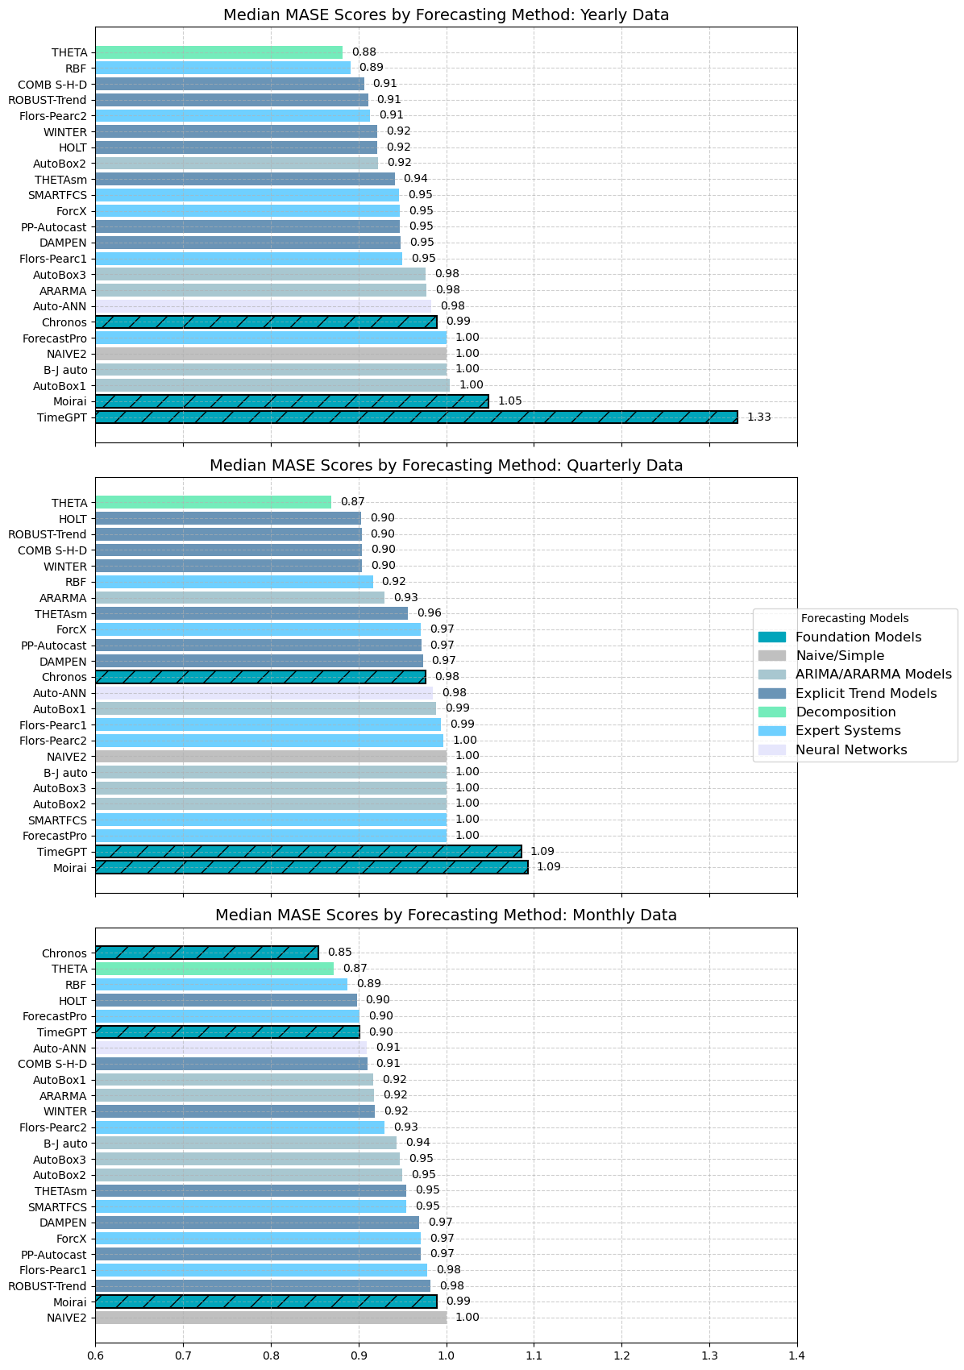
\includegraphics[width=0.8\textwidth]{mase_combined.png}
  \caption{Median MASE scores for different time frequencies.}
  \label{mase_combined_figure}
\end{figure}

As seen in Figure (\ref{mase_combined_figure}), the median MASE scores for the models are considerably worse for yearly data, with Chronos falling 13 places in ranking and TimeGPT being the worst-performing model by a $0.27$ margin. These MASE scores indicate that Moirai and TimeGPT perform worse than the Naïve2 benchmark within this subset, with Chronos narrowly avoiding the same outcome.

The three foundation models' performance is not convincing for quarterly data. While Chronos exhibits a minimal improvement of $0.01$ in the median MASE score, resulting in a modest rise in ranking, TimeGPT demonstrates better performance compared to its yearly counterpart but still falls short of achieving a favorable ranking. Moirai is the only one of the three models that performs worse quarterly than yearly, but only by a narrow margin. 


The median MASE scores changes significantly when analyzing monthly data, with Chronos becoming the top model in this subset. TimeGPT shows a notable improvement, nearly reaching the top five, in contrast to its last-place ranking for yearly data MASE scores. Additionally, \hyperref[appendix_d]{Appendix D} shows that the performance of TimeGPT can slightly improve through finetuning for this subset. In contrast, Moirai outperforms the Naive2 benchmark for the first time in our analysis by a small margin of just $0.01$. 

These observations are underscored by Figure \ref{mase_rmse_timefrequencies}, which depicts the variation in the mean MASE scores across the forecast period for the foundation models compared to the Naive2 benchmark. A consistent pattern emerges across all plots: the models underperform the benchmark for yearly data, perform closer to the benchmark for quarterly data, and beats the benchmark for monthly data.

\begin{figure}[htbp]
  \centering
  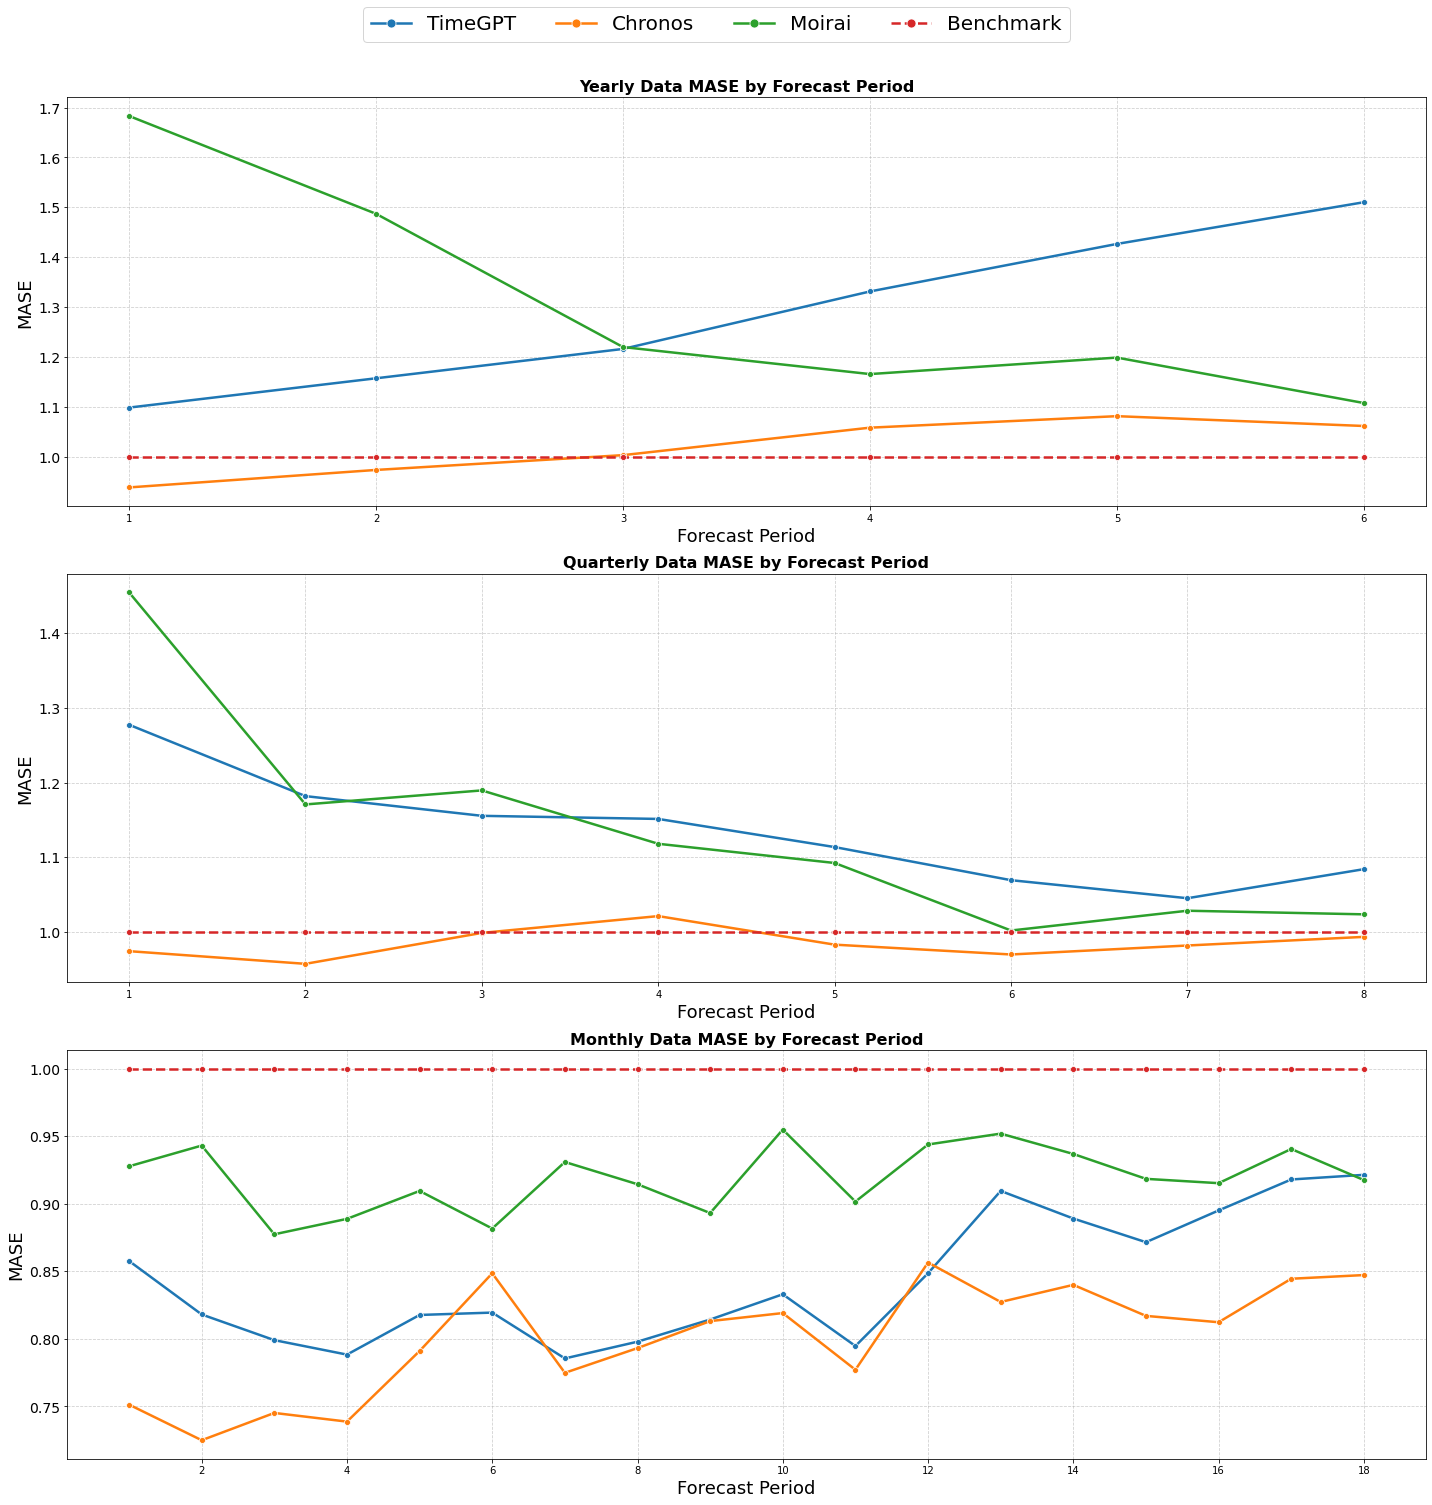
\includegraphics[width=0.8\textwidth]{mase_forecast_period_real.png}
  \caption{Mean MASE Scores at Each Forecast Step for Different Time Frequencies.}
  \label{mase_rmse_timefrequencies}
\end{figure}

An interesting trend emerges when examining the distributions of MASE scores for the three foundation models across the three time frequencies: the distribution narrows with increasing granularity. Earlier plots demonstrated how model performance improves as the data frequency shifts from yearly to quarterly to monthly. Figure (\ref{mase_distribution}) reveals that, in addition to the improvement in median MASE scores, the scores also become more tightly clustered around the median. The exception is Chronos for monthly data, where, despite the distribution being less concentrated than for quarterly data, the \textit{Interquartile Range} remains well below 1, indicating strong performance for monthly data compared to the benchmark.

\begin{figure}[htbp]
  \centering
  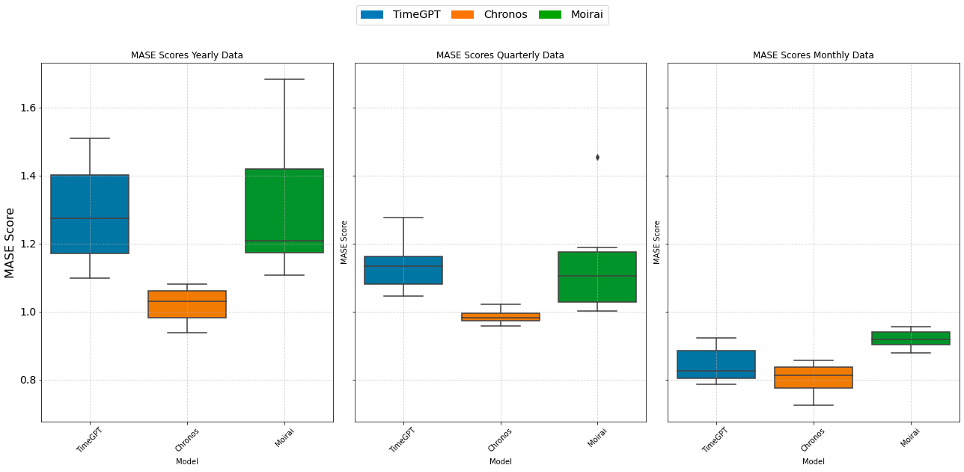
\includegraphics[width=0.8\textwidth]{mase_distributions_frequency.png}
  \caption{Distribution of MASE scores for different time frequencies.}
  \label{mase_distribution}
\end{figure}

\subsubsection{Categories}

The performance of the three foundation models varies across different data categories in the M3-Competition. Figure (\ref{mase_categories}) shows the median MASE scores for each model by category. Chronos demonstrates competitiveness with a median MASE score below one in all categories. TimeGPT and Moirai, however, fail to surpass the benchmark in two and four categories, respectively. They each outperform Chronos in only one category, with Moirai doing so by a margin of just 0.03. The most substantial differences between the models are observed in the demographic and macroeconomic categories, where Chronos clearly outperforms both TimeGPT and Moirai, which show similar performance to each other.

\begin{figure}[htbp]
  \centering
  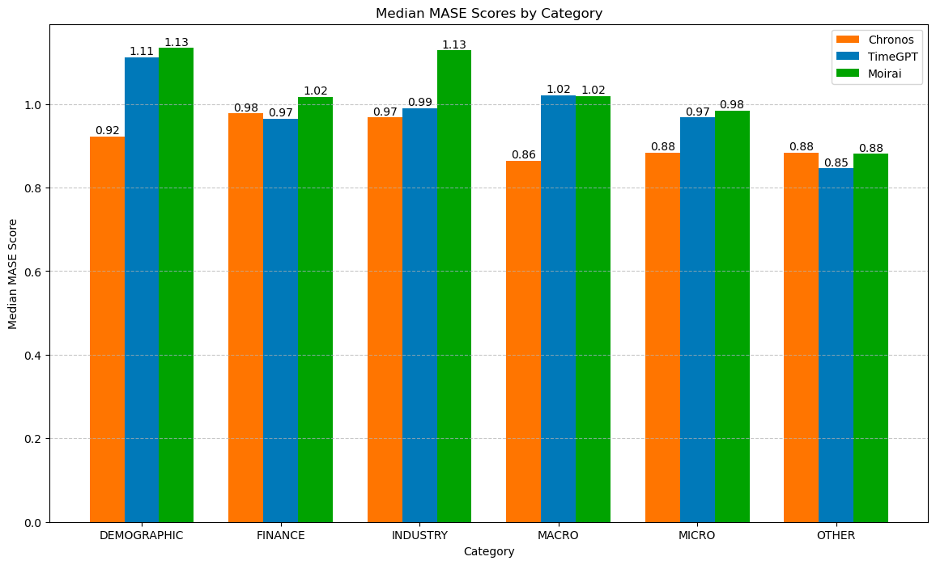
\includegraphics[width=0.8\textwidth]{mase_categories.png}
  \caption{Median MASE Scores for Different Categories.}
  \label{mase_categories}
\end{figure}

As previously demonstrated, the three foundation models are sensitive to the time frequency of the data. It is, therefore, of interest to see the categories for each subset of time frequency to better understand their performance. 

Table (\ref{mase_categories_table}) shows Chronos performing consistently well compared to the other two foundation models, particularly for finance, micro- and macroeconomic data where both the median and mean MASE score place well below the benchmark for monthly data. TimeGPT has a median MASE score below one for all categories in monthly data and nearly achieves this in mean MASE score, except for industry data. However, it performs remarkably poorly for yearly demographic and macroeconomic data compared to the other models, affecting its ranking in the previously mentioned leaderboard. In the median MASE scores, MOIRAI outperforms TimeGPT in all categories of yearly data. However, this does not hold for other time frequencies, except for quarterly macroeconomic data, where MOIRAI also beats TimeGPT. The category “Other” only contains eleven time series for yearly data and should not hold much weight in this evaluation. 


\begin{table}[h!tbp]
  \centering
  \caption{Median and Mean MASE Scores for Different Categories and Frequencies.}
  \label{mase_categories_table}
  \resizebox{\textwidth}{!}{%
  \begin{tabular}{llllllllll}
   &  & \multicolumn{2}{c}{Chronos} &  & \multicolumn{2}{c}{TimeGPT} &  & \multicolumn{2}{c}{Moirai} \\ \cmidrule(lr){3-4} \cmidrule(lr){6-7} \cmidrule(lr){9-10}
   &  & \textbf{median} & \textbf{mean} &  & \textbf{median} & \textbf{mean} &  & \textbf{median} & \textbf{mean} \\
  \textbf{Frequency} & \textbf{Category} &  &  &  &  &  &  &  &  \\ 
  \midrule
  \multirow{6}{*}{Monthly} & DEMOGRAPHIC & 0.87 & 1.16 &  & 0.95 & 0.97 &  & 1.11 & 1.21 \\
   & FINANCE & 0.86 & 0.92 &  & 0.87 & 0.85 &  & 0.98 & 1.07 \\
   & INDUSTRY & 0.98 & 1.05 &  & 0.93 & 1.01 &  & 1.11 & 1.19 \\
   & MACRO & 0.79 & 0.98 &  & 0.91 & 0.98 &  & 1.03 & 1.18 \\
   & MICRO & 0.79 & 0.82 &  & 0.88 & 0.88 &  & 0.92 & 0.93 \\
   & OTHER & 0.8 & 0.84 &  & 0.83 & 0.85 &  & 0.88 & 1.02 \\ 
  \midrule
  \multirow{5}{*}{Quarterly} & DEMOGRAPHIC & 1.06 & 1.11 &  & 0.99 & 1.26 &  & 1.05 & 1.41 \\
   & FINANCE & 1.02 & 1.12 &  & 1.01 & 1.21 &  & 1.05 & 1.1 \\
   & INDUSTRY & 0.96 & 1.06 &  & 1.13 & 1.45 &  & 1.28 & 1.56 \\
   & MACRO & 0.95 & 1.25 &  & 1.11 & 1.36 &  & 1.04 & 1.33 \\
   & MICRO & 0.97 & 1.09 &  & 1.09 & 1.31 &  & 1.15 & 1.38 \\ 
  \midrule
  \multirow{6}{*}{Yearly} & DEMOGRAPHIC & 0.93 & 1.14 &  & 1.51 & 2.2 &  & 1.18 & 1.8 \\
   & FINANCE & 1.06 & 1.28 &  & 1.13 & 1.32 &  & 1.06 & 1.49 \\
   & INDUSTRY & 0.95 & 1.08 &  & 1.15 & 1.43 &  & 1.1 & 1.87 \\
   & MACRO & 1.02 & 0.95 &  & 1.73 & 1.84 &  & 0.95 & 1.07 \\
   & MICRO & 1.01 & 1.2 &  & 1.29 & 1.45 &  & 1.04 & 1.27 \\
   & OTHER & 0.99 & 0.93 &  & 0.99 & 0.98 &  & 0.89 & 0.87 \\ 
  \bottomrule
  \end{tabular}%
  }
\end{table}


\subsubsection{Benchmark}

So far, we have used the MASE scores to evaluate the models’ performances. However, as we now directly compare the three foundation models to the benchmark, using MASE might confuse things as the MASE scores are already scaled to the benchmark performance. We use the Percentage Better and the differences in sMAPE scores to simplify the comparisons and provide additional insights. The Percentage Better metric indicates how often the foundation models outperform the benchmark. The differences in sMAPE scores provide a clear percentage-based error comparison between the models and the benchmark. 

Table (\ref{percentage_better_table}) illustrates the Percentage Better across different categories and time series frequencies, giving a view of model performance in varied contexts. We use a weighted average calculation for these percentages to ensure a fair comparison, accounting for varying sample sizes across categories and frequencies. This approach explains how often the foundation models outperform the Naïve2 benchmark.

\begin{table}[h!tbp]
  \centering
  \caption{Percentage Better than Naïve2 for Different Time Frequencies and Categories.}
  \label{percentage_better_table}
  \resizebox{\textwidth}{!}{%
  \begin{tabular}{lllllll}
  \toprule
  \textbf{Frequency} & \textbf{Category} & \textbf{\#Time Series} &  & \multicolumn{3}{c}{\textbf{Percentage Better}} \\ 
  \cmidrule(lr){5-7}
   &  &  &  & \textbf{Chronos} & \textbf{TimeGPT} & \textbf{Moirai} \\ 
  \midrule
  \multirow{6}{*}{Monthly} & DEMOGRAPHIC & 111 &  & 57.66 & 61.26 & 44.14 \\
   & FINANCE & 145 &  & 62.07 & 63.45 & 53.79 \\
   & INDUSTRY & 334 &  & 53.59 & 59.88 & 40.72 \\
   & MACRO & 312 &  & 69.55 & 64.42 & 46.79 \\
   & MICRO & 473 &  & 75.48 & 69.13 & 63.21 \\
   & OTHER & 52 &  & 67.31 & 67.31 & 57.69 \\ 
  \midrule
  \multirow{5}{*}{Quarterly} & DEMOGRAPHIC & 57 &  & 45.61 & 50.88 & 45.61 \\
   & FINANCE & 76 &  & 46.05 & 48.68 & 43.42 \\
   & INDUSTRY & 83 &  & 55.42 & 38.55 & 26.51 \\
   & MACRO & 336 &  & 53.57 & 41.96 & 46.43 \\
   & MICRO & 204 &  & 53.92 & 39.71 & 34.8 \\ 
  \midrule
  \multirow{6}{*}{Yearly} & DEMOGRAPHIC & 245 &  & 55.51 & 31.84 & 39.18 \\
   & FINANCE & 58 &  & 37.93 & 34.48 & 41.38 \\
   & INDUSTRY & 102 &  & 57.84 & 34.31 & 43.14 \\
   & MACRO & 83 &  & 46.99 & 7.23 & 60.24 \\
   & MICRO & 147 &  & 46.26 & 26.53 & 46.94 \\
   & OTHER & 11 &  & 63.64 & 54.55 & 90.91 \\ 
  \midrule
  \multicolumn{2}{l}{\textbf{Weighted Average}} &  &  & 59.03 & 50.44 & 47.33 \\ 
  \bottomrule
  \end{tabular}%
  }
\end{table}

Table (\ref{smape_scores_table}) shows a comparison of the sMAPE scores between a selection of models against Naive2 as the benchmark with averages for different time horizons (full comparison in \hyperref[appendix_c]{Appendix C}). Table (\ref{smape_scores_table}) underscores the competitiveness of Chronos. Equally, it reveals the shortcomings of TimeGPT and Moirai as contenders despite their improving performance with longer forecast horizons. The forecast horizon, inherently tied to the data frequency, reveals that the foundation models demonstrate progressively better performance as granularity increases. This supports the earlier finding that the foundation models’ performance improves for monthly data.

\begin{table}[h!tbp]
  \centering
  \caption{Differences in sMAPE Scores Against Benchmark.}
  \label{smape_scores_table}
  \begin{tabular}{llllll}
  \hline
  \textbf{Method} & \textbf{1} & \textbf{Avg 1-4} & \textbf{Avg 1-6} & \textbf{Avg 1-12} & \textbf{Avg 1-18} \\ \hline
  THETA & 2.15 & 2.23 & 2.09 & 2.37 & 2.54 \\
  ForecastPro & 1.93 & 2.02 & 1.85 & 2.18 & 2.40 \\
  Chronos & 1.92 & 1.87 & 1.54 & 2.10 & 2.41 \\
  ForcX & 1.87 & 1.86 & 1.86 & 2.10 & 2.01 \\
  DAMPEN & 1.77 & 1.58 & 1.50 & 1.90 & 1.93 \\
  COMB S-H-D & 1.66 & 1.56 & 1.54 & 1.97 & 2.10 \\
  RBF & 0.67 & 1.13 & 1.35 & 1.57 & 1.91 \\
  TimeGPT & 0.28 & -0.08 & -0.61 & 0.92 & 1.19 \\
  Moirai & -0.86 & -0.44 & -0.25 & 0.39 & 0.65 \\ \hline
  \end{tabular}
\end{table}

\subsection{Robustness of Results} \label{robustness}

To visualize how the performance of the three foundation models would have looked under different variations of the dataset from the M3-Competition, we draw 1,000 samples with a sample size of 500 in Figure (\ref{mase_sampling_distribution}). This further validates our findings, showing that if we were to evaluate the models on random data samples instead of the entire datasets, Chronos would be the preferred model in most cases.

\begin{figure}[htbp]
  \centering
  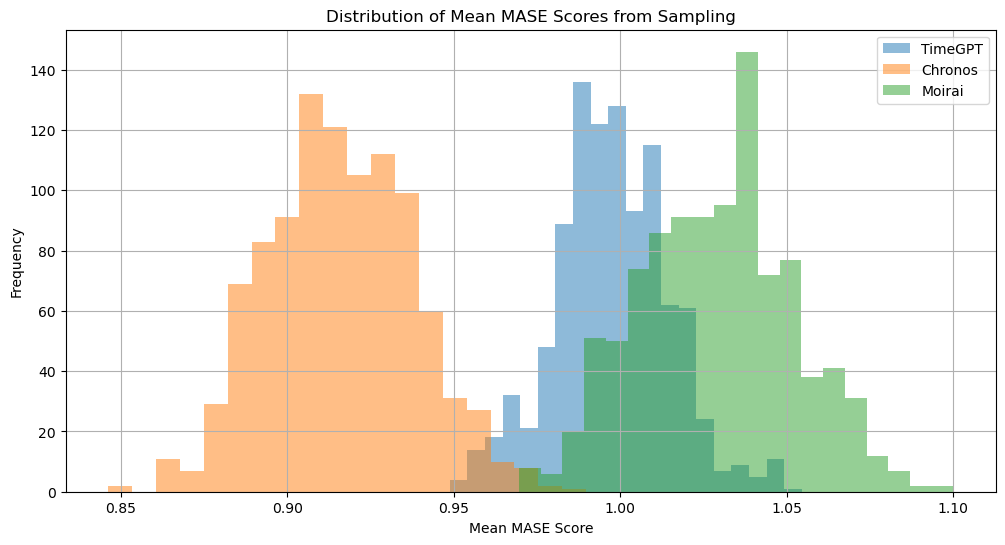
\includegraphics[width=0.8\textwidth]{real_bootstrap_sampling.png}
  \caption{Bootstrap Sampling Distribution of Median MASE Scores}
  \label{mase_sampling_distribution}
\end{figure}

The Friedman’s test reveals a statistically significant difference between the performance of the foundation models. The Wilcoxon Singed-rank test further confirms this is true for any combination of the three models. In addition, the Levene’s test shows that the variances of the three foundation models are unequal. The Wilcoxon Singed-rank test also discovers that all three foundation models perform significantly worse than Theta, the champion model in our evaluation. All statistical tests are done with a 5\% confidence interval. More details in \hyperref[appendix_e]{Appendix E}.

We conclude this section by investigating how the foundation models rank in MASE scores for each time series to see if the placement in the earlier leaderboard is justifiable. Figure (\ref{stacked_ranking_count}) shows the count of times each foundation model occupies each rank across all the time series.

\begin{figure}[htbp]
  \centering
  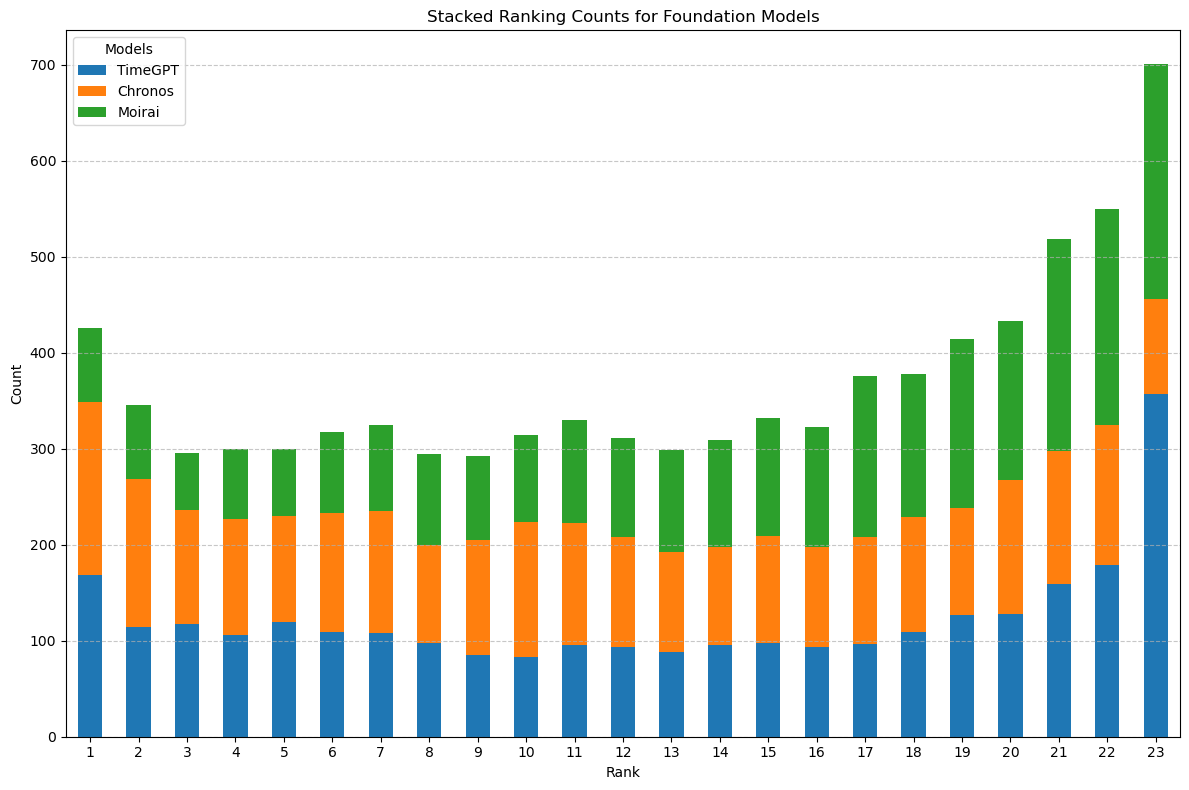
\includegraphics[width=0.8\textwidth]{real_stacked_counts.png}
  \caption{Stacked Barchart of \textit{Leaderboard} Placements of Foundation Models.}
  \label{stacked_ranking_count}
\end{figure}

Based on MASE rankings, TimeGPT and Moirai tend to place last more frequently than any other position, with the second-to-last position being their next most common ranking. This supports their low leaderboard rankings. TimeGPT ranks first 168 times, which equals 5.9\% of the time, making it the third most frequent position for this model. This indicates that TimeGPT can be useful in some cases compared to the other models despite their ranking. Moirai displays a clear trend of increasing counts for worse ranks, with the last three positions being the most frequent. Chronos ranks first most frequently, 6.4\% of the time, with second place as the second most frequent position. In fact, Chronos place more often in the top three than any other model in our selection. This justifies its higher leaderboard position. 

The plot shows that rankings vary significantly across time series for all three models. This suggests that the leaderboard should not be taken at face value, as the foundation models' performance varies significantly across the time series. For more details and additional figures, see \hyperref[appendix_e]{Appendix E}.

% \begin{center}
%   \section{Discussion}
% \end{center}
\newpage
{\centering \section{Discussion} \par}

\subsection{Discussion of Results}

The evaluation of the three foundation models—Chronos, TimeGPT, and Moirai—within the context of the M3-Competition demonstrates insights into their performance and characteristics. Overall, the models did not exceed expectations uniformly. Chronos achieved an impressive fifth place, whereas TimeGPT and Moirai placed in the last two positions. This indicates that while foundation models show promise, there is a large discrepancy in their performances.

One notable observation is the sensitivity of model performance to the time frequency of the data. All three models performed better with monthly data than quarterly and yearly data, with Chronos emerging as the champion model for monthly data. This trend may be attributed to the models being trained on data with more granular datasets. Furthermore, the distribution of MASE scores for the models narrows with increasing data granularity, indicating that the models perform better with higher frequency data. When comparing the models across different data categories, Chronos consistently outperformed the Naïve2 benchmark, demonstrating its robustness across varied types of data. In contrast, TimeGPT and Moirai performed worse and more varied, aligning with their performance in the different frequencies of data.

Among the three models, Chronos outperformed the others, demonstrating competitive performance in the M3-Competition. TimeGPT showed notable performance with monthly data but lacked the same competitiveness for yearly and quarterly data. Moirai, while the least competitive overall, still managed to exceed the benchmark nearly half the time, suggesting that even the low-performing model has potential value in certain contexts.

This evaluation highlights the strengths and weaknesses of the foundation models, emphasizing their varying performances across different data frequencies. While Chronos stands out as the most competitive model, Section (\ref{robustness}) reveals that our initial leaderboard should not be taken at face value, as both TimeGPT and MOIRAI perform well for certain time series.

\subsection{Limitations}

Despite the insights provided by our research in this thesis, several limitations should be acknowledged when judging our findings.

First, his thesis exclusively investigates how the foundation models perform in zero-shot forecasting. We do not fine-tune models or use exogenous variables, which could enhance the performance of what we present in our main results. Fine-tuning is a critical step when applying models in real-world scenarios, and its exclusions may limit the generalizability of our findings and do not accurately describe the models’ optimal performance. We do, however, present our experiment with fine-tuning TimeGPT in \hyperref[appendix_d]{Appendix D}, but this is for a subset of the data, and it would therefore be dishonest to give it any weight in our evaluation. 

Second, TimeGPT is not an open-source model, which limits transparency and reproducibility. The two other models in our evaluation, Chronos and Moirai, are relatively new and lack extensive documentation. This also limits the knowledge of the models despite our efforts to describe them to the best of our capabilities. It also caps the depth in understanding the models’ mechanisms and performance characteristics. 

Third, we utilize the M3-Competition dataset, which is reputable and relatively old. Therefore, the data does not necessarily represent current trends and reflect today's most relevant data sources. Also, the dataset is not particularly large. We deem the size to be big enough for this evaluation, but its size limits the ability to generalize our findings to more granular frequencies, such as daily or hourly data and complex streaming data. 

Lastly, we do not compare the foundation models to the performance of other advanced and sophisticated forecasting methods, such as gradient boosting or random forest models. While these methods have become widely popular, we have deemed this comparison unnecessary for the scope of this thesis, especially as the Theta model is included, which performed very well on the dataset. Nonetheless, the absence of these comparisons can be a limitation in demonstrating the relative performance of foundation models to other new and complex models.  

\subsection{Future Research}

While this thesis helps to better understand the performance of foundation models in zero-shot forecasting, future research on foundation models for time series forecasting could benefit from several different explorations. First, it would be interesting to replicate this study on a larger dataset or competition. Analyzing a more extensive and diverse dataset would help determine whether the observed results hold true across a broader spectrum of data and scenarios. Specifically, using weekly, daily, and even hourly data could provide valuable insights into whether model performance continues to improve with higher frequency data, as suggested by our findings with monthly data. 

Additionally, exploring the adaptation and evolution of foundation models and other AI models in the coming years will be crucial. Staying current on upcoming developments and assessing their implications for time series forecasting will be important. New models and techniques are constantly emerging, and it would be of significant interest to the scientific community and practitioners to research what technologies are being adopted, how easily they can be integrated, and what factors contribute to breakthroughs in this field.

It would be valuable to compare these foundation models with other innovative approaches, such as the recently introduced xLSTM modifications to LSTM by \cite{beck2024xlstm}. New developments in model architecture are emerging for both Large Language Models and Computer Vision applications. It will be interesting to examine how well these architectures apply to time series, especially considering how well Chronos performed in this study despite minimal efforts to modify the architecture for time series data. This comparison could provide deeper insights into the potential advantages and limitations of different model architectures in handling time series data.

Another promising area for future research is the application of explainable AI (XAI) techniques to foundation models in time series forecasting. Understanding the decision-making processes of these complex models is essential for building trust and understanding their utility in real-world applications. Advancements in large language models (LLMs) are ongoing, as demonstrated by recent work from \cite{templeton2024scaling}, which shows that interpretable features can be extracted from \textit{Claude 3}, a popular LLM. Researchers can strengthen their applicability and reliability in various forecasting scenarios by developing methods to make the predictions of foundation models more transparent and interpretable.

In summary, future research should focus on expanding the scope of data and competitions to validate current findings, continuously adapting to advancements in AI, and emphasizing interpretability to ensure that foundation models are effective and trustworthy in time series forecasting. These directions will help pave the way for more robust, adaptable, and transparent forecasting models.

% \begin{center}
%   \item  \section{Conclusion}
% \end{center}
\newpage
{\centering \section{Conclusion} \par}

This thesis evaluates the zero-shot forecasting performance of foundation models using the M3-Competition dataset. Utilizing the MASE metric, we compare these models against the Naïve2 benchmark, a simpler forecasting method, to determine if the foundation models offer superior performance.

The analysis reveals that none of the three foundation models outperform the original competition's champion, the Theta model. However, the foundation model Chronos stands out, ranking fifth overall and surpassing the benchmark, indicating significant promise, especially as an open-source option. In contrast, the other two models, TimeGPT and Moirai, performed worse, ranking at the bottom of our initial ranking. This is particularly interesting because Chronos employs a minimalistic approach to time series forecasting, unlike the other two models. It makes only minor adaptations to a large language model and is the only model trained on synthetic data.

The frequency of the data strongly impacts the models' performance. The foundation models performed similarly to or worse than the benchmark for yearly and quarterly data, indicating their unsuitability for these data types. Conversely, the models, particularly Chronos and TimeGPT, performed better for monthly data, with Chronos emerging as the best performer among all models. The performance of these models was also more stable for monthly data, suggesting a potential use case for foundation models in this context.

Using foundation models for zero-shot forecasting appears to be a viable approach, though model choice is important. Performance varies by data type, with established methods preferred for yearly and quarterly data. However, foundation models such as Chronos and TimeGPT show strong performance for monthly data, with Chronos notably outperforming all models within this subset. Given its outstanding performance, practitioners should be encouraged to consider Chronos as an option for monthly data forecasting. 


\newpage
\printbibliography{}
\addcontentsline{toc}{section}{Bibliography}

\newpage
\begin{center}
\item  \section*{Appendix A} \label{appendix_a}
\end{center}

\addcontentsline{toc}{section}{Appendix A}


\begin{center}
  \item  \subsection*{Methods used in the M3-Competition}
\end{center}

Table (\ref{forecast_methods_table}) shows an overview of the methods used in the M3 Competition with the short descriptions of \cite{MAKRIDAKIS2000}. A longer description of most of the models, those that is not used in earlier M- Competitions, can be found in the appendix of the paper. Further explanation of the Robust-Trend and ARARMA methodologies used is provided by \cite{Meade2000}.


\begin{table}[htbp]
  \centering
  \caption{Description of Forecasting Methods Used in the M3-Competition.}
  \label{forecast_methods_table}
  \resizebox{\textwidth}{!}{%
  \begin{tabular}{lp{2cm}lp{10cm}}
  \toprule
  \textbf{Category} & \textbf{Methods} & \textbf{Competitors} & \textbf{Description} \\ 
  \midrule
  \multirow{2}{*}{Naïve/ Simple} & Naïve 2 & M. Hibon & Naïve forecast where seasonality is first removed. \\
  & Single & M. Hibon & Single Exponential Smoothing. \\ 
  \midrule
  \multirow{8}{*}{Explicit Trend Models} & Holt & M. Hibon & Automatic Holt’s Linear Exponential smoothing. \\
  & Robust-Trend & N. Meade & Nonparametric version of Holt’s linear model with median based estimate of trend. \\
  & Winter & M. Hibon & Holt-Winter’s linear and seasonal exponential smoothing. \\
  & Dampen & M. Hibon & Dampen Trend Exponential Smoothing. \\
  & PP autocast & H. Levenbach & Dampen Trend Exponential Smoothing. \\
  & THETA-sm & V. Assimakopoulos & Successive smoothing plus a set of rules for dampening the trend. \\
  & Comb S/H/D & M. Hibon & Combining Single/Holt/Dampen methods. \\ 
  \midrule
  \multirow{1}{*}{Decomposition} & THETA & V. Assimakopoulos & Specific decomposition technique, projection and combination of the individual components. \\ 
  \midrule
  \multirow{7}{*}{ARIMA/ ARARMA Models} & BJ-automatic & M. Hibon & Box Jenkins methodology of “Business Forecast System”. \\
  & AUTOBOX 1 & D. Reilly & Robust ARIMA univariate Box-Jenkins with/without Intervention Detection. \\
  & AUTOBOX 2 & D. Reilly & Robust ARIMA univariate Box-Jenkins with/without Intervention Detection. \\
  & AUTOBOX 3 & D. Reilly & Robust ARIMA univariate Box-Jenkins with/without Intervention Detection. \\
  & AAM 1 & G. Melard \& J. M. Pasteels & Automatic ARIMA modeling with/without intervention analysis. \\
  & AAM 2 & G. Melard \& J. M. Pasteels & Automatic ARIMA modeling with/without intervention analysis. \\
  & ARARMA & N. Meade & Automated Parzen’s methodology with Auto regressive filter. \\ 
  \midrule
  \multirow{6}{*}{Expert Systems} & ForecastPRO & R. Goodrich \& E. Stellwagen & Selects from among several methods: Exponential Smoothing/Box Jenkins/Poisson and negative binominal models/Croston’s method/Simple Moving Average. \\
  & SMARTFCs & C. Smart & Automatic Forecasting Expert System which conducts a forecasting tournament among 4 Exponential Smoothing and 2 Moving Average methods. \\
  & RBF & M. Adya, S. Armstrong, F. Collopy \& M. Kennedy & Rule-Based forecasting: using 3 methods – random walk, linear regression and Holt’s to estimate level and trend, involving corrections, simplification, automatic feature identification and recalibration. \\
  & FLORES-PEARCE1 & B. Flores \& S. Pearce & Expert system that chooses among 4 methods based on the characteristics of the data. \\
  & FLORES-PEARCE2 & B. Flores \& S. Pearce & Expert system that chooses among 4 methods based on the characteristics of the data. \\
  & ForecastX & J. Galt & Runs tests for seasonality and outliers and selects from among several methods: Exponential Smoothing, Box-Jenkins and Croston’s method. \\ 
  \midrule
  \multirow{1}{*}{Neural Networks} & Automat ANN & K. Ord \& S. Balkin & Automated Artificial Neural Networks for forecasting purposes. \\ 
  \bottomrule
  \end{tabular}%
  }
\end{table}

\newpage

\begin{center}
  \item  \section*{Appendix B} \label{appendix_b}
\end{center}

\addcontentsline{toc}{section}{Appendix B}

\subsection*{Data Distribution By Category}


\begin{figure}[htbp]
  \centering
  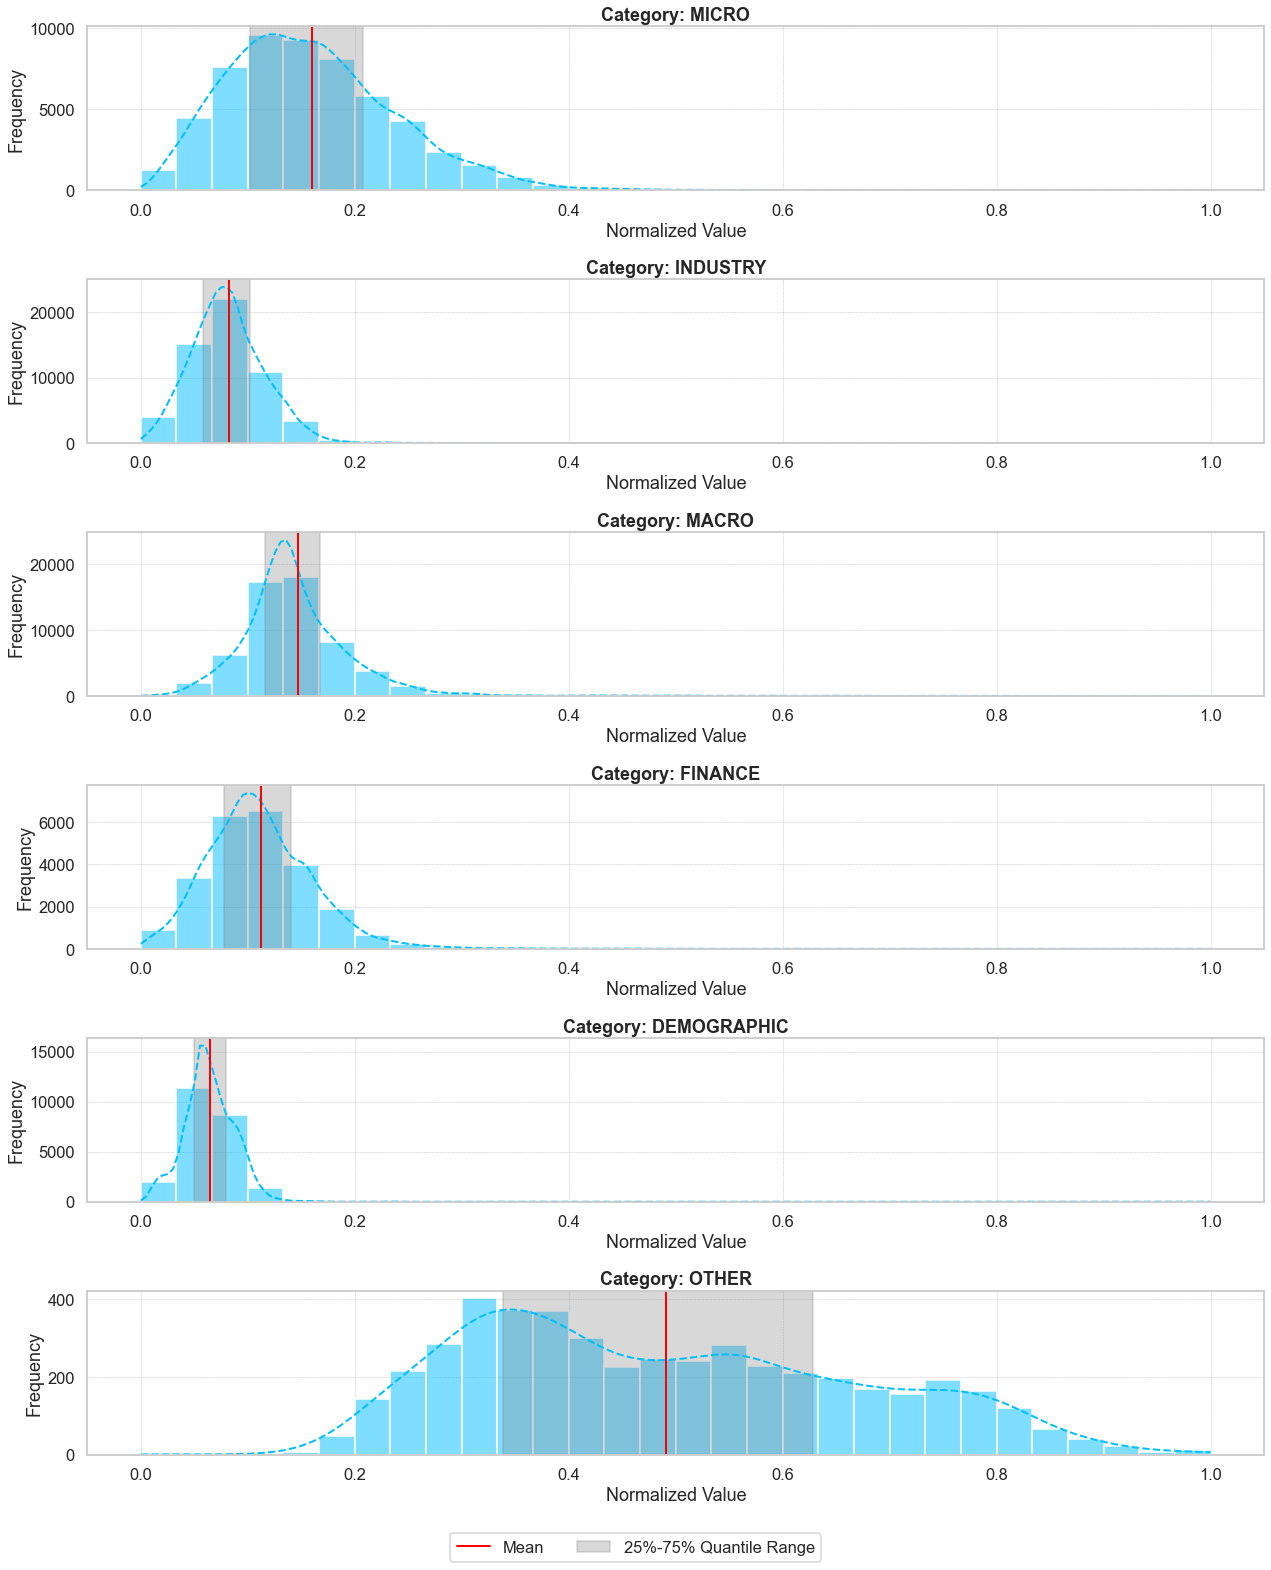
\includegraphics[width=0.8\textwidth]{real_distributions_data_descr.png}
  \caption{Dsitribution of the M3-Competition Data by Category.}
  \label{m3_distribution}
\end{figure}

\newpage

\begin{center}
  \item  \section*{Appendix C} \label{appendix_c}
\end{center}

\addcontentsline{toc}{section}{Appendix C}

\subsection*{Additional Results}


In this appendix, we provide the scores in other evaluation metrics. This is not intended as a supplementary analysis, but simply offers the reader the opportunity to evaluate the performance of the models in style with the original M3-Competition. We do not rely on findings from these metrics in our evaluation as they can be more sensitive to skewness and outliers. However, the following three tables support our findings with Chronos being in the top three when averaging for all forecast horizons (Avg 1-18) regardless of forecasting metric, while TimeGPT and Moirai falls short.

% Average sMAPE 
\begin{table}[htbp]
  \centering
  \caption{Average Symmetric MAPE with All Data.}
  \resizebox{\columnwidth}{!}{%
  \begin{tabular}{lllllllllllllllllllllllllll}
  \hline
  Method & \multicolumn{18}{l}{Forecast Horizon} &  & \multicolumn{6}{l}{Average of Forecast Horizon} & \# obs \\ \hline
   & 1 & 2 & 3 & 4 & 5 & 6 & 7 & 8 & 9 & 10 & 11 & 12 & 13 & 14 & 15 & 16 & 17 & 18 &  & Avg 1-4 & Avg 1-6 & Avg 1-8 & Avg 1-12 & Avg 1-15 & Avg 1-18 &  \\ \hline
  NAIVE2 & 10.96 & 11.8 & 14.14 & 15.6 & 15.51 & 16.3 & 14.95 & 14.93 & 15.85 & 15.95 & 16.73 & 15.99 & 18.09 & 18.41 & 19.32 & 21.29 & 19.64 & 20.7 &  & 13.13 & 14.05 & 14.27 & 14.89 & 15.64 & 16.45 & 2829 \\
  SINGLE & 9.9 & 11.05 & 13.18 & 14.59 & 14.72 & 15.36 & 13.74 & 13.65 & 13.88 & 14.0 & 14.81 & 14.52 & 16.19 & 17.21 & 18.32 & 20.18 & 18.44 & 19.37 &  & 12.18 & 13.13 & 13.27 & 13.62 & 14.34 & 15.17 & 2829 \\
  HOLT & 9.41 & 10.93 & 13.49 & 15.44 & 16.16 & 16.92 & 14.75 & 14.93 & 14.4 & 15.67 & 15.4 & 15.32 & 17.15 & 17.85 & 19.45 & 20.07 & 20.07 & 21.06 &  & 12.32 & 13.72 & 14.0 & 14.4 & 15.15 & 16.03 & 2829 \\
  DAMPEN & 9.19 & 10.4 & 12.54 & 14.08 & 14.26 & 14.85 & 13.22 & 12.98 & 13.21 & 13.34 & 14.0 & 13.85 & 15.63 & 16.26 & 17.49 & 19.43 & 17.8 & 18.87 &  & 11.55 & 12.55 & 12.69 & 12.99 & 13.69 & 14.52 & 2829 \\
  WINTER & 9.55 & 11.0 & 13.65 & 15.52 & 16.21 & 17.03 & 14.77 & 15.06 & 14.6 & 15.66 & 15.5 & 15.24 & 17.22 & 17.9 & 19.58 & 20.18 & 20.01 & 21.07 &  & 12.43 & 13.83 & 14.1 & 14.48 & 15.23 & 16.1 & 2829 \\
  COMB S-H-D & 9.3 & 10.45 & 12.53 & 14.0 & 14.16 & 14.62 & 13.09 & \textbf{12.9} & 13.07 & 13.58 & 13.69 & 13.63 & 15.41 & 16.19 & 17.28 & 18.85 & 17.36 & \textbf{18.26} &  & 11.57 & 12.51 & 12.63 & 12.92 & 13.59 & 14.35 & 2829 \\
  B-J auto & 9.65 & 10.86 & 12.69 & 14.42 & 14.51 & 15.2 & 13.52 & 13.44 & 13.41 & 13.38 & 14.52 & 14.06 & 16.25 & 16.94 & 17.76 & 19.72 & 18.15 & 19.26 &  & 11.9 & 12.89 & 13.04 & 13.3 & 14.04 & 14.87 & 2829 \\
  AutoBox1 & 10.3 & 11.59 & 13.65 & 15.77 & 16.62 & 17.4 & 14.86 & 14.77 & 14.36 & 14.33 & 15.49 & 15.36 & 17.53 & 18.1 & 19.09 & 20.42 & 20.18 & 20.39 &  & 12.83 & 14.22 & 14.37 & 14.54 & 15.28 & 16.12 & 2829 \\
  AutoBox2 & 10.02 & 10.87 & 12.76 & 14.51 & 14.43 & 15.47 & 14.21 & 13.81 & 14.63 & 14.7 & 15.53 & 15.18 & 17.56 & 17.41 & 18.37 & 20.74 & 19.01 & 19.99 &  & 12.04 & 13.01 & 13.26 & 13.84 & 14.63 & 15.51 & 2829 \\
  AutoBox3 & 10.23 & 11.82 & 13.62 & 15.48 & 16.79 & 17.38 & 15.53 & 15.43 & 14.93 & 15.81 & 16.12 & 16.68 & 18.52 & 18.32 & 19.83 & 21.54 & 22.6 & 21.99 &  & 12.79 & 14.22 & 14.54 & 14.99 & 15.77 & 16.81 & 2829 \\
  ROBUST-Trend & 11.03 & 11.73 & 13.91 & 15.42 & 15.76 & 16.64 & 15.75 & 16.0 & 18.28 & 18.69 & 18.82 & 18.05 & 20.93 & 21.46 & 23.24 & 24.1 & 23.21 & 25.75 &  & 13.02 & 14.08 & 14.53 & 15.84 & 17.05 & 18.26 & 2829 \\
  ARARMA & 10.19 & 11.39 & 13.12 & 14.81 & 15.14 & 16.21 & 14.53 & 14.55 & 14.87 & 15.01 & 15.85 & 15.21 & 17.51 & 17.25 & 18.48 & 20.01 & 18.66 & 20.32 &  & 12.38 & 13.48 & 13.74 & 14.24 & 14.94 & 15.73 & 2829 \\
  Auto-ANN & 9.45 & 10.98 & 12.37 & 14.45 & 14.46 & 16.24 & 13.84 & 14.0 & 13.96 & 14.89 & 14.71 & 14.81 & 17.03 & 16.83 & 17.55 & 19.29 & 18.25 & 19.81 &  & 11.81 & 12.99 & 13.22 & 13.68 & 14.37 & 15.16 & 2829 \\
  Flors-Pearc1 & 9.61 & 10.91 & 13.14 & 15.04 & 15.28 & 15.82 & 14.7 & 14.33 & 14.43 & 14.29 & 14.59 & 14.43 & 16.68 & 18.19 & 19.13 & 21.22 & 20.13 & 21.01 &  & 12.18 & 13.3 & 13.6 & 13.88 & 14.7 & 15.72 & 2829 \\
  Flors-Pearc2 & 10.49 & 11.48 & 13.32 & 14.61 & 14.56 & 15.2 & 13.58 & 13.41 & 13.26 & 13.82 & 14.31 & 14.37 & 16.42 & 17.59 & 18.23 & 20.12 & 18.49 & 20.24 &  & 12.48 & 13.28 & 13.33 & 13.53 & 14.31 & 15.19 & 2829 \\
  PP-Autocast & 9.56 & 10.56 & 12.71 & 14.21 & 14.48 & 15.24 & 13.82 & 13.86 & 14.58 & 14.29 & 15.19 & 14.39 & 16.47 & 16.99 & 17.93 & 19.78 & 18.3 & 19.85 &  & 11.76 & 12.79 & 13.05 & 13.57 & 14.29 & 15.12 & 2829 \\
  ForecastPro & \textbf{9.03} & \textbf{9.98} & \textbf{11.89} & \textbf{13.54} & 13.92 & 14.85 & 12.96 & 13.14 & \textbf{13.02} & \textbf{13.0} & 13.9 & \textbf{13.31} & \textbf{15.28} & \textbf{15.43} & \textbf{16.43} & 18.17 & \textbf{16.8} & 18.29 &  & \textbf{11.11} & \textbf{12.2} & \textbf{12.41} & 12.71 & \textbf{13.31} & \textbf{14.05} & 2829 \\
  SMARTFCS & 9.59 & 10.69 & 12.45 & 14.05 & 14.53 & 15.59 & 13.67 & 13.51 & 13.86 & 15.19 & 15.01 & 14.94 & 16.55 & 16.58 & 18.01 & 18.43 & 19.32 & 19.42 &  & 11.7 & 12.82 & 13.01 & 13.59 & 14.28 & 15.08 & 2829 \\
  THETAsm & 9.91 & 11.1 & 13.09 & 14.34 & 15.31 & 16.21 & 14.51 & 13.9 & 14.47 & 14.81 & 14.83 & 14.38 & 16.7 & \textbf{15.7} & 17.72 & 19.26 & 18.07 & 19.28 &  & 12.11 & 13.33 & 13.55 & 13.9 & 14.47 & 15.2 & 2829 \\
  THETA & \textbf{8.81} & \textbf{9.99} & \textbf{11.77} & \textbf{13.03} & \textbf{13.66} & \textbf{14.5} & \textbf{12.8} & \textbf{12.45} & 13.17 & 13.4 & \textbf{13.48} & \textbf{13.23} & \textbf{15.42} & \textbf{15.23} & \textbf{16.36} & \textbf{17.77} & 16.88 & 18.36 &  & \textbf{10.9} & \textbf{11.96} & \textbf{12.13} & \textbf{12.52} & \textbf{13.15} & \textbf{13.91} & 2829 \\
  RBF & 10.29 & 10.95 & 12.88 & 13.88 & \textbf{13.62} & \textbf{14.58} & 13.65 & 13.19 & 14.16 & 14.47 & 14.14 & 14.05 & 16.1 & 15.78 & \textbf{17.26} & \textbf{18.28} & \textbf{16.76} & \textbf{17.76} &  & 12.0 & 12.7 & 12.88 & 13.32 & 13.93 & 14.54 & 2829 \\
  ForcX & 9.09 & 10.26 & \textbf{12.09} & \textbf{13.65} & \textbf{13.7} & \textbf{14.37} & \textbf{12.9} & 13.06 & 13.06 & 13.43 & 13.89 & 13.97 & 15.77 & 16.65 & 17.85 & 19.35 & 18.13 & 18.79 &  & 11.27 & \textbf{12.19} & \textbf{12.39} & \textbf{12.79} & 13.58 & 14.44 & 2829 \\
  Chronos & \textbf{9.04} & \textbf{9.95} & 12.21 & 13.84 & 14.15 & 15.87 & \textbf{12.75} & \textbf{12.86} & \textbf{12.86} & \textbf{13.19} & \textbf{13.27} & \textbf{13.48} & \textbf{15.37} & 15.77 & \textbf{15.97} & \textbf{17.63} & \textbf{16.49} & \textbf{18.07} &  & \textbf{11.26} & 12.51 & 12.58 & \textbf{12.79} & \textbf{13.37} & \textbf{14.04} & 2829 \\
  TimeGPT & 10.68 & 11.84 & 14.04 & 16.26 & 16.75 & 18.41 & 13.25 & 13.3 & \textbf{12.86} & \textbf{13.26} & \textbf{13.42} & 13.6 & 16.59 & 16.62 & 17.3 & 19.65 & 17.96 & 18.91 &  & 13.21 & 14.66 & 14.32 & 13.97 & 14.55 & 15.26 & 2829 \\
  Moirai & 11.82 & 12.84 & 14.17 & 15.46 & 15.52 & 15.98 & 14.62 & 14.03 & 14.0 & 15.1 & 15.33 & 15.1 & 17.38 & 17.11 & 18.16 & 20.11 & 18.45 & 19.24 &  & 13.57 & 14.3 & 14.31 & 14.5 & 15.11 & 15.8 & 2829 \\ \hline
  \end{tabular}%
  }
  \vspace{1ex}
  {\raggedright \footnotesize{\textit{Note:} Top Three Scores in Each Column are Bolded}. \par}
\end{table}


% MEDIAN APE

\begin{table}[]
  \centering
  \caption{Median Absolute Percentage Error with All Data.}
  \resizebox{\columnwidth}{!}{%
  \begin{tabular}{lllllllllllllllllllllllllll}
  \hline
  Method & \multicolumn{18}{l}{Forecast Horizon} &  & \multicolumn{6}{l}{Average of Forecast Horizon} & \# obs \\ \hline
   & 1 & 2 & 3 & 4 & 5 & 6 & 7 & 8 & 9 & 10 & 11 & 12 & 13 & 14 & 15 & 16 & 17 & 18 &  & Avg 1-4 & Avg 1-6 & Avg 1-8 & Avg 1-12 & Avg 1-15 & Avg 1-18 &  \\ \hline
  NAIVE2 & 3.66 & 4.75 & 6.05 & 7.06 & 7.57 & 8.47 & 7.67 & 7.7 & 7.82 & 8.22 & 8.39 & 7.79 & 9.35 & 9.49 & 10.24 & 10.92 & 10.82 & 11.62 &  & 5.38 & 6.26 & 6.62 & 7.1 & 7.62 & 8.2 & 2829 \\
  HOLT & 3.35 & 4.33 & 5.39 & 6.59 & 7.19 & 7.42 & 6.6 & 6.55 & 6.43 & 7.46 & 6.89 & 7.23 & 8.26 & \textbf{7.47} & \textbf{8.75} & \textbf{9.13} & 9.29 & 10.32 &  & 4.92 & 5.71 & 5.93 & 6.29 & 6.66 & 7.15 & 2829 \\
  DAMPEN & 3.28 & \textbf{4.04} & 5.1 & 6.51 & 6.79 & 7.42 & 6.81 & 6.88 & 6.73 & 6.8 & 6.73 & 7.47 & 8.28 & 8.27 & 9.69 & 10.4 & 9.75 & 10.51 &  & \textbf{4.73} & 5.52 & 5.85 & 6.21 & 6.72 & 7.3 & 2829 \\
  WINTER & 3.42 & 4.37 & 5.5 & 6.51 & 7.25 & 7.49 & 6.66 & 6.84 & 6.5 & 7.23 & 7.06 & 7.04 & 8.52 & 7.81 & 9.05 & \textbf{9.26} & 9.36 & 10.14 &  & 4.95 & 5.76 & 6.01 & 6.32 & 6.75 & 7.22 & 2829 \\
  COMB S-H-D & 3.35 & 4.18 & 5.15 & 6.47 & 6.8 & 7.19 & 6.58 & 6.7 & 6.43 & 6.84 & 6.7 & \textbf{6.87} & 8.26 & 8.1 & 9.05 & 9.39 & \textbf{9.13} & 9.83 &  & 4.79 & 5.52 & 5.8 & 6.1 & 6.58 & \textbf{7.06} & 2829 \\
  B-J auto & 3.29 & 4.23 & 5.37 & 6.6 & 6.78 & 7.26 & 6.56 & 6.48 & 6.86 & 6.94 & 6.64 & 7.19 & 8.24 & 8.55 & 9.21 & 10.44 & 9.65 & 10.65 &  & 4.87 & 5.59 & 5.82 & 6.18 & 6.68 & 7.27 & 2829 \\
  AutoBox1 & 3.72 & 4.66 & 5.75 & 6.61 & 7.22 & 7.93 & 6.64 & 7.03 & 6.45 & 6.76 & 7.2 & 7.04 & 8.5 & 8.2 & 9.17 & 9.73 & 9.75 & 10.55 &  & 5.18 & 5.98 & 6.2 & 6.42 & 6.86 & 7.38 & 2829 \\
  AutoBox2 & 3.39 & 4.41 & 5.22 & 6.35 & \textbf{6.43} & 7.23 & 6.78 & \textbf{6.36} & 6.77 & 6.71 & 6.81 & 7.09 & 8.38 & 8.57 & 9.41 & 9.99 & 9.4 & 10.26 &  & 4.84 & 5.5 & 5.77 & 6.13 & 6.66 & 7.2 & 2829 \\
  AutoBox3 & 3.62 & 4.74 & 5.7 & 6.8 & 7.17 & 7.74 & 6.87 & 7.27 & 6.9 & 7.03 & 6.98 & 7.08 & 9.06 & 8.4 & 8.91 & 10.05 & 10.31 & 10.45 &  & 5.22 & 5.96 & 6.24 & 6.49 & 6.95 & 7.5 & 2829 \\
  ROBUST-Trend & 3.5 & 4.37 & 5.24 & 6.28 & 7.1 & 7.55 & 7.17 & 7.13 & 7.67 & 8.32 & 8.64 & 7.47 & 8.87 & 8.87 & 9.72 & 10.02 & 10.49 & 11.68 &  & 4.85 & 5.67 & 6.04 & 6.7 & 7.19 & 7.78 & 2829 \\
  ARARMA & 3.42 & 4.4 & 5.32 & 6.64 & 7.07 & 7.83 & 6.56 & 7.01 & 7.16 & 6.93 & 6.91 & 7.08 & 8.14 & 8.42 & 8.85 & 9.49 & 9.28 & 10.18 &  & 4.94 & 5.78 & 6.03 & 6.36 & 6.78 & 7.26 & 2829 \\
  Auto-ANN & 3.4 & 4.64 & 5.55 & 6.82 & 7.16 & 7.88 & 6.89 & 7.06 & 7.06 & 7.35 & 7.05 & 7.38 & 8.64 & 9.09 & 9.53 & 10.27 & 9.83 & 11.13 &  & 5.1 & 5.91 & 6.18 & 6.52 & 7.03 & 7.6 & 2829 \\
  Flors-Pearc1 & 3.49 & 4.11 & 5.13 & 6.6 & 6.99 & 7.31 & 7.14 & 7.0 & 6.64 & 7.28 & 6.88 & 7.46 & 8.65 & 8.98 & 9.8 & 10.15 & 10.13 & 10.73 &  & 4.83 & 5.6 & 5.97 & 6.34 & 6.9 & 7.47 & 2829 \\
  Flors-Pearc2 & 4.41 & 4.96 & 5.7 & 7.06 & 6.96 & \textbf{7.17} & 6.58 & 6.94 & 6.42 & 7.09 & 6.74 & 7.62 & 8.14 & 8.61 & 9.52 & 9.96 & 9.72 & 10.43 &  & 5.53 & 6.04 & 6.22 & 6.47 & 6.93 & 7.45 & 2829 \\
  PP-Autocast & \textbf{3.18} & 4.14 & 5.37 & 6.72 & 7.06 & 7.6 & 6.93 & 6.75 & 6.92 & 7.01 & 7.13 & 7.37 & 8.28 & 8.7 & 9.84 & 10.44 & 10.13 & 10.98 &  & 4.85 & 5.68 & 5.97 & 6.35 & 6.87 & 7.48 & 2829 \\
  ForecastPro & \textbf{3.19} & 4.09 & \textbf{4.86} & \textbf{6.21} & \textbf{6.54} & 7.19 & \textbf{6.3} & 6.53 & \textbf{6.19} & \textbf{6.43} & 6.63 & \textbf{6.65} & \textbf{7.69} & \textbf{7.69} & 8.62 & 9.55 & 8.97 & \textbf{9.66} &  & 4.59 & \textbf{5.35} & \textbf{5.61} & \textbf{5.9} & \textbf{6.32} & 6.83 & 2829 \\
  SMARTFCS & 3.94 & 4.63 & 5.42 & 6.55 & 6.8 & 7.26 & 6.58 & \textbf{6.43} & 6.5 & 7.76 & 7.43 & 7.64 & 8.87 & 8.19 & 8.98 & 9.38 & 10.5 & 10.14 &  & 5.14 & 5.77 & 5.95 & 6.41 & 6.87 & 7.39 & 2829 \\
  THETAsm & 3.64 & 4.61 & 5.85 & 6.75 & 7.29 & 8.05 & 7.06 & 7.18 & 7.14 & 7.61 & 7.71 & 7.83 & 9.01 & 8.21 & 9.63 & 10.74 & 10.09 & 10.91 &  & 5.21 & 6.03 & 6.3 & 6.73 & 7.17 & 7.74 & 2829 \\
  THETA & 3.23 & \textbf{3.95} & \textbf{4.93} & \textbf{5.9} & 6.59 & \textbf{6.92} & \textbf{6.21} & \textbf{6.21} & 6.57 & \textbf{6.67} & \textbf{6.35} & \textbf{6.86} & \textbf{7.96} & \textbf{7.72} & 8.32 & 9.5 & 8.81 & \textbf{9.77} &  & \textbf{4.5} & \textbf{5.25} & \textbf{5.49} & \textbf{5.87} & \textbf{6.29} & \textbf{6.8} & 2829 \\
  RBF & 4.28 & 4.86 & 5.59 & 6.51 & 7.11 & 7.44 & 6.98 & 6.59 & 6.79 & 7.47 & 7.09 & 6.9 & 8.17 & 7.89 & 8.73 & 9.44 & \textbf{9.01} & \textbf{9.39} &  & 5.31 & 5.96 & 6.17 & 6.47 & 6.83 & 7.24 & 2829 \\
  ForcX & 3.33 & 4.08 & \textbf{4.97} & \textbf{6.2} & \textbf{6.47} & \textbf{7.0} & \textbf{6.28} & 6.52 & \textbf{6.31} & 6.91 & \textbf{6.23} & 7.43 & 8.22 & 8.61 & 9.24 & 10.31 & 9.82 & 10.14 &  & \textbf{4.64} & \textbf{5.34} & \textbf{5.61} & \textbf{5.98} & 6.52 & 7.11 & 2829 \\
  Chronos & \textbf{3.22} & \textbf{4.0} & 5.23 & 6.51 & 6.78 & 7.5 & 6.37 & 6.56 & 6.59 & \textbf{6.6} & \textbf{6.6} & 6.89 & \textbf{7.52} & 8.03 & \textbf{8.7} & \textbf{9.12} & \textbf{8.72} & 10.12 &  & 4.74 & 5.54 & 5.77 & 6.07 & \textbf{6.47} & \textbf{6.95} & 2829 \\
  TimeGPT & 4.25 & 5.15 & 6.35 & 7.63 & 7.97 & 8.55 & 7.15 & 6.9 & \textbf{6.33} & 6.79 & \textbf{6.6} & 6.93 & 8.31 & 8.15 & \textbf{8.51} & 10.35 & 9.74 & 10.44 &  & 5.84 & 6.65 & 6.74 & 6.72 & 7.04 & 7.56 & 2829 \\
  Moirai & 5.46 & 6.08 & 6.69 & 7.83 & 7.87 & 8.4 & 7.3 & 7.34 & 7.49 & 8.23 & 7.96 & 7.96 & 9.46 & 8.88 & 9.97 & 10.46 & 9.91 & 10.99 &  & 6.52 & 7.06 & 7.12 & 7.38 & 7.79 & 8.24 & 2829 \\ \hline
  \end{tabular}%
  }
  \vspace{1ex}
  {\raggedright \footnotesize{\textit{Note:} Top Three Scores in Each Column are Bolded}. \par}
\end{table}

% MEDIAN RAE

\begin{table}[]
  \centering
  \caption{Median Relative Absolute Error with All Data.}
  \resizebox{\columnwidth}{!}{%
  \begin{tabular}{llllllllllllllllllllllllllll}
  \hline
  Method & \multicolumn{18}{l}{Forecast Horizon} &  & \multicolumn{6}{l}{Average of Forecast Horizon} & \# obs \\ \hline
   & 1 & 2 & 3 & 4 & 5 & 6 & 7 & 8 & 9 & 10 & 11 & 12 & 13 & 14 & 15 & 16 & 17 & 18 &  & Avg 1-4 & Avg 1-6 & Avg 1-8 & Avg 1-12 & Avg 1-15 & Avg 1-18 &  \\ \hline
  
  NAIVE2 & 0.18 & 0.2 & 0.25 & 0.31 & 0.32 & 0.35 & 0.32 & 0.33 & 0.32 & 0.33 & 0.3 & 0.29 & 0.33 & 0.32 & 0.34 & 0.35 & 0.36 & 0.37 &  & 0.24 & 0.27 & 0.28 & 0.29 & 0.3 & 0.31 & 2829 \\
  HOLT & 0.16 & 0.19 & 0.23 & 0.28 & 0.29 & 0.31 & 0.29 & \textbf{0.28} & \textbf{0.24} & 0.3 & \textbf{0.24} & 0.25 & \textbf{0.27} & \textbf{0.26} & \textbf{0.29} & \textbf{0.31} & 0.32 & 0.33 &  & 0.22 & 0.24 & 0.25 & 0.26 & 0.26 & 0.27 & 2829 \\
  DAMPEN & 0.16 & \textbf{0.18} & \textbf{0.22} & 0.27 & 0.29 & 0.3 & \textbf{0.27} & 0.29 & \textbf{0.25} & \textbf{0.28} & 0.27 & 0.27 & 0.3 & 0.28 & 0.31 & 0.34 & 0.33 & 0.35 &  & 0.21 & 0.24 & 0.25 & \textbf{0.25} & 0.26 & 0.28 & 2829 \\
  WINTER & 0.16 & 0.19 & 0.24 & 0.28 & 0.3 & 0.31 & 0.28 & \textbf{0.28} & \textbf{0.25} & 0.3 & 0.26 & \textbf{0.24} & \textbf{0.27} & \textbf{0.26} & 0.3 & \textbf{0.31} & 0.33 & \textbf{0.32} &  & 0.22 & 0.25 & 0.26 & 0.26 & 0.26 & 0.27 & 2829 \\
  COMB S-H-D & 0.16 & 0.19 & 0.23 & 0.27 & 0.28 & 0.3 & \textbf{0.27} & \textbf{0.28} & \textbf{0.25} & 0.3 & 0.25 & 0.25 & 0.28 & 0.27 & 0.3 & 0.32 & 0.32 & 0.33 &  & 0.21 & 0.24 & 0.25 & 0.25 & 0.26 & 0.27 & 2829 \\
  B-J auto & 0.16 & 0.19 & 0.23 & 0.27 & 0.29 & 0.3 & 0.28 & 0.29 & 0.27 & \textbf{0.28} & 0.28 & 0.27 & 0.3 & 0.31 & 0.31 & 0.36 & 0.32 & 0.35 &  & 0.21 & 0.24 & 0.25 & 0.26 & 0.27 & 0.28 & 2829 \\
  AutoBox1 & 0.17 & 0.2 & 0.24 & 0.28 & 0.3 & 0.32 & \textbf{0.27} & 0.29 & 0.26 & \textbf{0.28} & 0.26 & 0.26 & 0.3 & 0.3 & 0.31 & 0.33 & 0.34 & 0.34 &  & 0.22 & 0.25 & 0.26 & 0.26 & 0.27 & 0.28 & 2829 \\
  AutoBox2 & 0.17 & 0.19 & 0.23 & 0.28 & 0.28 & 0.31 & 0.29 & 0.29 & 0.26 & \textbf{0.28} & 0.26 & 0.26 & 0.29 & 0.29 & 0.31 & 0.34 & 0.34 & 0.35 &  & 0.22 & 0.24 & 0.26 & 0.26 & 0.27 & 0.28 & 2829 \\
  AutoBox3 & 0.16 & 0.21 & 0.24 & 0.29 & 0.3 & 0.32 & 0.29 & 0.29 & 0.26 & 0.29 & 0.25 & 0.25 & 0.29 & 0.28 & 0.3 & 0.33 & 0.35 & 0.35 &  & 0.22 & 0.25 & 0.26 & 0.26 & 0.27 & 0.28 & 2829 \\
  ROBUST-Trend & 0.17 & 0.2 & 0.24 & 0.27 & 0.29 & 0.3 & 0.29 & 0.31 & 0.31 & 0.32 & 0.3 & 0.27 & 0.3 & 0.33 & 0.34 & 0.34 & 0.34 & 0.37 &  & 0.22 & 0.24 & 0.26 & 0.27 & 0.28 & 0.29 & 2829 \\
  ARARMA & 0.16 & 0.19 & 0.24 & 0.27 & 0.28 & 0.31 & 0.28 & 0.3 & 0.27 & 0.29 & 0.26 & 0.26 & 0.28 & 0.28 & 0.3 & 0.33 & 0.33 & 0.35 &  & 0.22 & 0.24 & 0.25 & 0.26 & 0.26 & 0.28 & 2829 \\
  Auto-ANN & 0.16 & 0.2 & \textbf{0.22} & 0.28 & 0.29 & 0.33 & 0.28 & 0.29 & 0.26 & 0.3 & 0.27 & 0.26 & 0.3 & 0.3 & 0.31 & 0.33 & 0.33 & 0.34 &  & 0.22 & 0.25 & 0.26 & 0.26 & 0.27 & 0.28 & 2829 \\
  Flors-Pearc1 & 0.16 & 0.19 & 0.23 & 0.28 & 0.3 & 0.31 & 0.29 & 0.3 & 0.26 & 0.29 & 0.27 & 0.27 & 0.31 & 0.31 & 0.33 & 0.35 & 0.35 & 0.37 &  & 0.22 & 0.24 & 0.26 & 0.26 & 0.27 & 0.29 & 2829 \\
  Flors-Pearc2 & 0.19 & 0.22 & 0.25 & 0.29 & 0.3 & 0.31 & 0.28 & 0.29 & \textbf{0.25} & \textbf{0.28} & 0.26 & 0.29 & 0.3 & 0.3 & 0.32 & 0.33 & 0.34 & 0.36 &  & 0.24 & 0.26 & 0.27 & 0.27 & 0.28 & 0.29 & 2829 \\
  PP-Autocast & 0.16 & 0.19 & 0.23 & 0.27 & 0.29 & 0.31 & 0.28 & 0.29 & 0.27 & 0.31 & 0.28 & 0.27 & 0.3 & 0.29 & 0.31 & 0.34 & 0.34 & 0.36 &  & 0.21 & 0.24 & 0.25 & 0.26 & 0.27 & 0.28 & 2829 \\
  ForecastPro & \textbf{0.15} & \textbf{0.18} & \textbf{0.21} & \textbf{0.25} & \textbf{0.27} & \textbf{0.29} & \textbf{0.27} & \textbf{0.27} & \textbf{0.24} & \textbf{0.26} & \textbf{0.24} & \textbf{0.23} & 0.28 & \textbf{0.26} & \textbf{0.28} & 0.33 & \textbf{0.31} & 0.33 &  & \textbf{0.2} & \textbf{0.22} & \textbf{0.24} & \textbf{0.24} & \textbf{0.25} & \textbf{0.26} & 2829 \\
  SMARTFCS & 0.17 & 0.2 & 0.24 & 0.28 & 0.29 & 0.31 & 0.28 & \textbf{0.28} & \textbf{0.25} & 0.32 & 0.27 & 0.27 & 0.3 & 0.27 & 0.31 & 0.32 & 0.34 & 0.34 &  & 0.22 & 0.25 & 0.26 & 0.26 & 0.27 & 0.28 & 2829 \\
  THETAsm & 0.17 & 0.2 & 0.24 & 0.28 & 0.3 & 0.32 & 0.28 & 0.3 & 0.28 & 0.31 & 0.28 & 0.27 & 0.3 & 0.27 & 0.3 & 0.32 & 0.32 & \textbf{0.32} &  & 0.22 & 0.25 & 0.26 & 0.27 & 0.27 & 0.28 & 2829 \\
  THETA & \textbf{0.15} & \textbf{0.18} & \textbf{0.21} & \textbf{0.25} & \textbf{0.27} & \textbf{0.28} & \textbf{0.26} & \textbf{0.27} & 0.26 & \textbf{0.28} & 0.25 & \textbf{0.24} & \textbf{0.27} & \textbf{0.26} & \textbf{0.29} & \textbf{0.31} & \textbf{0.31} & 0.33 &  & \textbf{0.2} & \textbf{0.22} & \textbf{0.23} & \textbf{0.24} & \textbf{0.25} & \textbf{0.26} & 2829 \\
  RBF & 0.2 & 0.21 & 0.24 & 0.27 & \textbf{0.28} & 0.3 & 0.28 & \textbf{0.28} & 0.27 & 0.31 & 0.25 & 0.25 & \textbf{0.27} & \textbf{0.25} & \textbf{0.29} & \textbf{0.31} & \textbf{0.31} & \textbf{0.31} &  & 0.23 & 0.25 & 0.26 & 0.26 & 0.26 & 0.27 & 2829 \\
  ForcX & \textbf{0.15} & \textbf{0.18} & 0.23 & \textbf{0.26} & \textbf{0.28} & \textbf{0.29} & \textbf{0.27} & \textbf{0.28} & \textbf{0.25} & \textbf{0.28} & 0.25 & 0.26 & 0.3 & 0.29 & 0.31 & 0.34 & 0.32 & 0.33 &  & \textbf{0.2} & \textbf{0.23} & \textbf{0.24} & \textbf{0.25} & 0.26 & 0.27 & 2829 \\
  Chronos & 0.16 & \textbf{0.18} & \textbf{0.22} & \textbf{0.26} & \textbf{0.28} & 0.31 & \textbf{0.26} & \textbf{0.28} & \textbf{0.25} & \textbf{0.25} & \textbf{0.24} & 0.25 & \textbf{0.26} & 0.27 & \textbf{0.28} & 0.32 & \textbf{0.29} & \textbf{0.31} &  & \textbf{0.2} & 0.24 & \textbf{0.24} & \textbf{0.25} & \textbf{0.25} & \textbf{0.26} & 2829 \\
  TimeGPT & 0.2 & 0.21 & 0.27 & 0.3 & 0.33 & 0.36 & 0.28 & 0.3 & \textbf{0.25} & \textbf{0.28} & 0.25 & 0.26 & 0.31 & 0.28 & 0.3 & 0.34 & 0.33 & 0.36 &  & 0.24 & 0.28 & 0.28 & 0.27 & 0.28 & 0.29 & 2829 \\
  Moirai & 0.24 & 0.26 & 0.28 & 0.3 & 0.32 & 0.35 & 0.31 & 0.32 & 0.28 & 0.34 & 0.29 & 0.28 & 0.33 & 0.31 & 0.33 & 0.35 & 0.34 & 0.37 &  & 0.27 & 0.29 & 0.3 & 0.3 & 0.3 & 0.31 & 2829 \\ \hline
  \end{tabular}%
  }
  \vspace{1ex}
  {\raggedright \footnotesize{\textit{Note:} Top Three Scores in Each Column are Bolded}. \par}
\end{table}
  
\newpage

\begin{center}
  \item  \section*{Appendix D} \label{appendix_d}
\end{center}

\addcontentsline{toc}{section}{Appendix D}

\subsection*{Fine-Tuning TimeGPT Experiment}
TimeGPT allows for straightforward fine-tuning, offering a choice between various loss functions such as MAE, MSE, RMSE, MAPE, and SMAPE. During fine-tuning, you can specify the desired loss function and the number of iterations, which indicates how many times the model will train on the provided data before generating forecasts.

Although our thesis primarily focuses on zero-shot forecasting, we were curious about the fine-tuning capabilities of the foundation model. To explore this, we conducted a small experiment to assess its impact. This experiment was limited to monthly data, as previous evaluations indicated that the model performs poorly with yearly and quarterly data. The results showed a slight improvement, with the MASE decreasing from 0.902 to 0.894. In this experiment, we performed 10 fine-tuning iterations and did not specify a loss function, aligning with our philosophy that foundation models should be easy to use.

\begin{figure}[htbp]
  \centering
  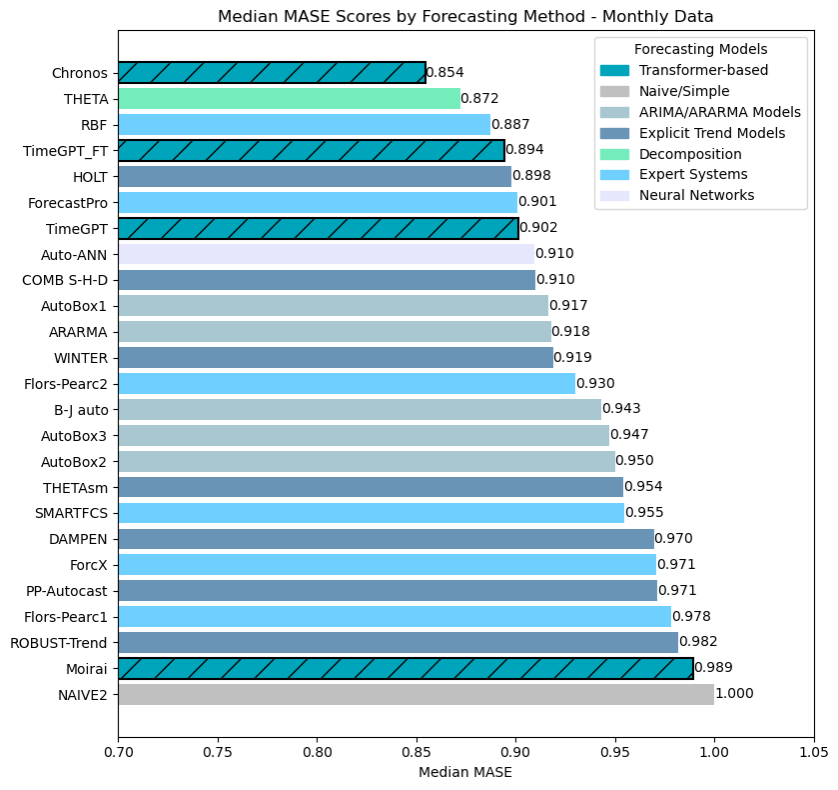
\includegraphics[width=0.8\textwidth]{timegpt_finetune_fig.png}
  \caption{Fine-Tuned TimeGPT on Monthly Data}
  \label{timegpt_finetune_fig}
\end{figure}

\newpage

\begin{center}
  \item  \section*{Appendix E} \label{appendix_e}
\end{center}

\addcontentsline{toc}{section}{Appendix E}

\subsection*{Robustness Checks}

\begin{figure}[htbp]
  \centering
  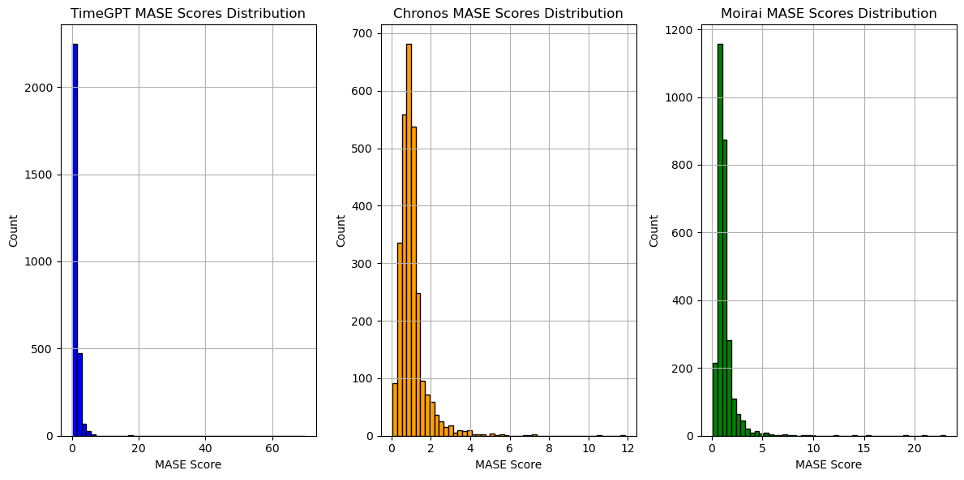
\includegraphics[width=0.8\textwidth]{mase_distribution_e.png}
  \caption{Distributions of MASE Scores for Foundation Models}
  \label{mase_distribution_e}
\end{figure}

\begin{figure}[htbp]
  \centering
  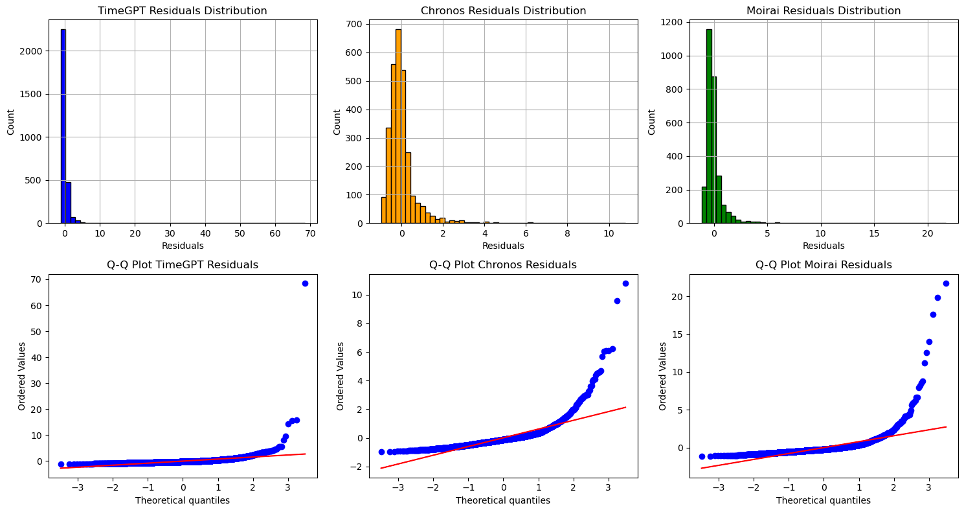
\includegraphics[width=0.8\textwidth]{residuals_distribution_e.png}
  \caption{Distributions of Residuals for Foundation Models (MASE Scores)} 
  \label{residuals_distribution_e}
\end{figure}

\paragraph*{Results of Friedman's Test}

For the group consisting of MASE Scores for TimeGPT, Moirai and Chronos:

Friedman’s Test Statistic: $247.96818663839076$, $p$-value: $1.426896352175751e-54$

Conclusion: There is a statistically significant difference between the models.

\paragraph*{Results of Levene's Test}

For the group consisting of MASE Scores for TimeGPT, Moirai and Chronos:

Levene's Test Statistic: $4.808090348578604$, $p$-value: $0.008185691864333012$

Reject the null hypothesis - variances are not equal (\textit{heteroscedasticity}).

\paragraph{Results of Wilcoxon Signed-Rank Test}

Only the tests where we accept the null hypothesis when comparing a selection of models.
We refer to the \href{https://github.com/tom-alten/Outsmarting-Time/}{GitHub} to see the test statistics for all comparisons drawn from the selection.
The selection consists of: Theta, Naive2, TimeGPT, Chronos, Moirai, ForecastPro, ForcX, Dampen, COMB S-H-D and RBF.

\underline{Wilcoxon Signed-Rank Test between Chronos and RBF:}

Test Statistic: $1962836.0$, $p$-value: $0.3733125068089125$

Fail to reject the null hypothesis - the median of the differences in the matched pairs is equal to 0

\underline{Wilcoxon Signed-Rank Test between ForcastPro and ForcX:}

Test Statistic: $1770965.0$, $p$-value: $0.14662673332067305$

Fail to reject the null hypothesis - the median of the differences in the matched pairs is equal to 0

\underline{Wilcoxon Signed-Rank Test between ForcastPro and COMB S-H-D:}

Test Statistic: $1969052.0$, $p$-value: $0.4549310940170622$

Fail to reject the null hypothesis - the median of the differences in the matched pairs is equal to 0

\underline{Wilcoxon Signed-Rank Test between ForcX and Dampen:}

Test Statistic: $1911761.0$, $p$-value: $0.06057003599052172$

Fail to reject the null hypothesis - the median of the differences in the matched pairs is equal to 0

\underline{Wilcoxon Signed-Rank Test between ForcX and RBF:}

Test Statistic: $1919268.0$, $p$-value: $0.058352805926870525$

Fail to reject the null hypothesis - the median of the differences in the matched pairs is equal to 0

\underline{Wilcoxon Signed-Rank Test between Dampen and RBF:}

Test Statistic: $1961356.0$, $p$-value: $0.3553046027801884$

Fail to reject the null hypothesis - the median of the differences in the matched pairs is equal to 0

\begin{figure}[htbp]
  \centering
  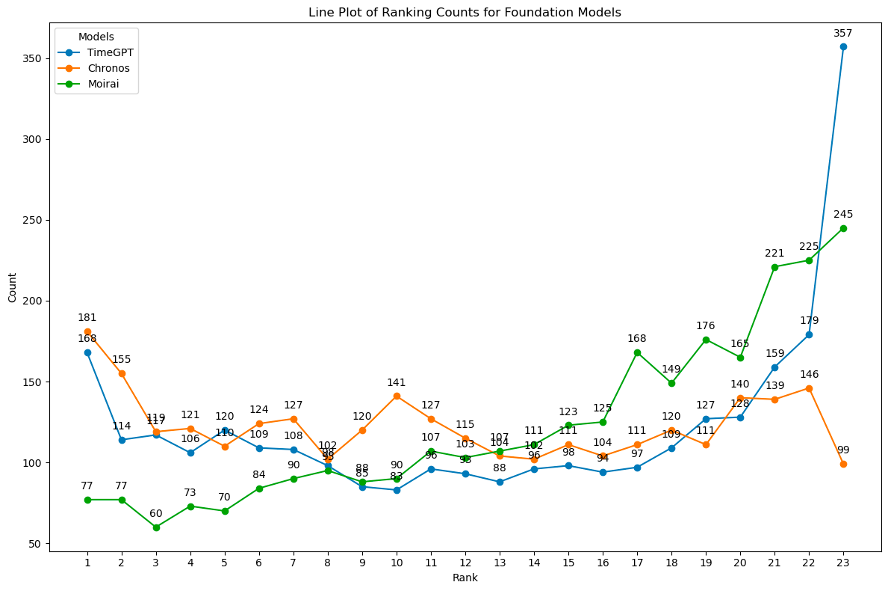
\includegraphics[width=0.8\textwidth]{counts_of_rank_lineplot.png}
  \caption{Counts of Ranking for Foundation Models as Line Plot} 
  \label{counts_of_rank_lineplot}
\end{figure}

\begin{figure}[htbp]
  \centering
  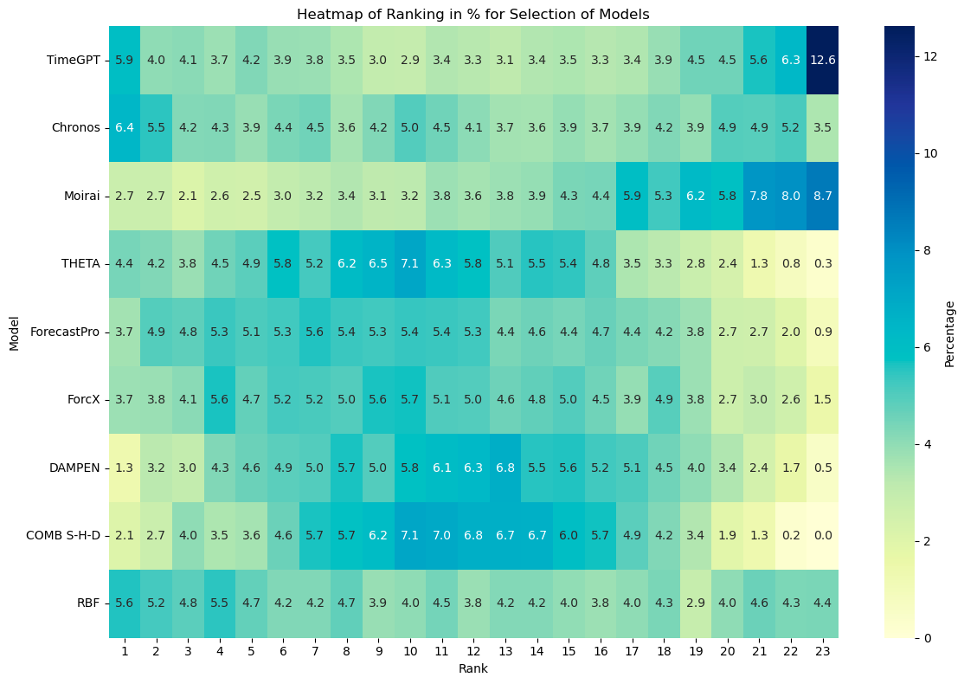
\includegraphics[width=0.8\textwidth]{heatmap.png}
  \caption{Heatmap of Rankings in \% for Selection of Models} 
  \label{heatmap}
\end{figure}

\end{document}